\documentclass[10pt]{article}
% MAXIMUM VIEWER COMPATIBILITY. pdfTeX writes PDF 1.5 by default, which uses a
% compressed cross reference stream and object streams. Both are legal and both
% are what GitHub's in browser viewer most often fails to render, reporting the
% file as invalid when it is not. Dropping to 1.4 with object compression off
% writes a classic xref table, which every viewer reads. It costs some file size
% and nothing else.
\pdfminorversion=4
\pdfobjcompresslevel=0
\pdfcompresslevel=9

\usepackage[margin=1in]{geometry}
\usepackage{amsmath,amssymb}
\usepackage{booktabs}
\usepackage{graphicx}
\usepackage{array}
\usepackage{rotating}% Table 6 on a landscape page (review item 15)
\usepackage[hidelinks]{hyperref}
\expandafter\def\expandafter\UrlBreaks\expandafter{\UrlBreaks\do-}% long URLs may break at a hyphen
\usepackage{xcolor}
% colour carried across a page break inside a footnote leaked into the body (2 October: Section 6 printed red)
\usepackage{pdfcolfoot}
% Everything revised in this draft is marked in red: the move to two periods and
% the responses to the comments on the previous version. The change of
% terminology from "the disorder" to "a SUD" runs through the whole note and is
% NOT marked, since colouring every instance would colour half the document.
% fill.py wraps in every number that MOVED against numbers_prev.json, so
% the note marks a changed number automatically rather than by hand. Set it to red
% so a recalibration shows up as red without anyone having to find the numbers.
% To clear the marks, copy the current numbers over numbers_prev.json and refill.
% is the mark fill.py puts on every number that moved since
% numbers_prev.json. It prints as ordinary text: the reader asked not to see the
% pipeline's own bookkeeping in red. The mark survives in the generated .tex,
% so grepping the generated file for the macro finds what moved, and grepping
% .src.tex for the at signs finds every number the stylized pipeline still
% supplies and the quantitative model has yet to replace.
% \textcolor is NOT \long: a red span that crossed a blank line died with
% "Paragraph ended before \@textcolor was complete", and pdflatex then
% returned nonzero, which set -e turned into a build that stopped before
% every checker in build.sh. \color is a switch and survives \par.
% \new MUST RENDER RED. strip_red.py rewrites this line to a passthrough,
% \newcommand{\new}[1]{#1}, so that any \new left after a strip is inert.
% That passthrough was committed once and every \new written afterwards
% went in as plain black text: several rounds of marked edits were
% invisible to the reader, in the intro, the calibration entries and the
% citations alike, while table cells kept showing red because they use
% \textcolor directly. check_red.py now fails the build if this line is
% a passthrough while any \new remains in the file.
\newcommand{\new}[1]{{\color{red}#1}}
% WHAT THE NEXT SIMULATIONS CHANGE (2 October): \upd tags a paragraph or a sentence, \updnum colours a number or a
% generated sentence that will be refilled. Blue, so they are never confused with the red of an edit; the red
% strippers leave them alone, and each goes when its paragraph is rewritten from the new runs.
\usepackage{marginnote}
% each \upd also flags the margin (marginnote works in minipages and floats, where \marginpar does not) and
% enters the list printed after the abstract, with its page, so every pending update can be found and clicked to
% HIDDEN IN THE PDF (the author, 6 October: "remove the blue I see in the pdf but keep placeholders for yourself for
% things you need to check/update"). The \upd tags and \updnum marks stay in the source as the list of what the next
% simulations refresh -- grep for them -- but print nothing (\upd, \listofupdates) or plain black (\updnum) while
% \showupdatesfalse. Set \showupdatestrue to see them in blue again.
\newif\ifshowupdates \showupdatesfalse
\newcommand{\upd}[1]{\ifshowupdates\phantomsection\addcontentsline{upd}{subsection}{#1}%
  \marginnote{\color{blue}\textbf{UPDATE}}{\color{blue}\textbf{[UPDATE: #1]}}\fi\ignorespaces}
\makeatletter
\newcommand{\listofupdates}{\ifshowupdates\par\noindent{\color{blue}\textbf{Pending updates from the new simulations}}\par
  {\small\@starttoc{upd}}\fi}
\makeatother
\newcommand{\updnum}[1]{\ifshowupdates{\color{blue}#1}\else#1\fi}
% WHAT A ROUND DELETED, AND WHY IT CHANGED (the author, 3 October: "deleted sentences should show as crossed so I
% know what you delete", and "leave notes for me in case I need to understand why you made a change"). \del prints
% deleted text struck through in red; \why prints a note in green and lists it, with its page, after the abstract.
% Both go, contents and all, when red is stripped (writing/marks.py), and the checkers do not read them.
\usepackage[normalem]{ulem}
\DeclareRobustCommand{\del}[1]{\sout{#1}}
\definecolor{whygreen}{rgb}{0,0.45,0.2}
\newcommand{\why}[1]{\phantomsection\addcontentsline{why}{subsection}{#1}%
  {\color{whygreen}\footnotesize[Why: #1]}}
% \green{...}: text the author asked to keep in green (8 October, on the custody sentence: "keep in green").
% Not a red mark, so strip_red.py leaves it; it stays green until the author says otherwise.
\newcommand{\green}[1]{{\color{whygreen}#1}}
\makeatletter
\newcommand{\listofwhys}{\ifshowupdates\par\noindent{\color{whygreen}\textbf{Notes on this round's changes}}\par
  {\small\@starttoc{why}}\fi}
\makeatother
% A number not computed yet: a slot to fill, never a guess.
\newcommand{\blank}{\underline{\hspace{2.2em}}}
% A STANDING FLAG, which survives the strip between rounds. \new and \cut both
% mark what changed since the last version and are cleared when the next round
% starts, so neither can carry an open question forward. \query holds one: a
% short red note in the margin asking whether a passage should be there at all.
% It is not prose and must be gone before the note is circulated.
% A FLAG IS A FOOTNOTE, NOT A MARGIN NOTE, AND THAT IS NOT A STYLE CHOICE.
% As a \marginpar it broke float placement: the run reported "Float(s) lost",
% the standard parameters table was never placed, its \label went with it, and
% the three references to it printed as ??. That is the same ?? flagged in the
% margin two rounds ago and explained away then as a stale build; it was this.
% Rebuilt with \query made a no-op the run is clean, which is what identifies
% the cause. Blue, so a flag is never mistaken for a round's red.
\newcommand{\query}[1]{\footnote{\textcolor{blue}{#1}}}
% THE PARAMETER COUNTS AS MACROS, so the two table files can quote them too.
% fill.py only rewrites its placeholders in this file, and the tables are
% \input from
% their own .tex, so a caption saying how many rows its table has could not be
% generated any other way. Counted off the Set column of the tables themselves.
\newcommand{\nmain}{@@n_main@@}
\newcommand{\nstd}{@@n_std@@}
% The cut macro below marks a PROPOSED DELETION: red and struck through, so the reader sees what
% would go before it goes. ulem is not in this installation, and a single rule over a
% whole phrase cannot break across lines, so the rule is drawn word by word: each word
% is its own box and TeX breaks between them as usual. The scanner below splits the
% argument on spaces, which is why a cut must not contain a braced group with a space
% inside it. Maths is fine, $14.2$ is one word.
\makeatletter
\newlength{\cw@len}
\newcommand{\cw}[1]{{\settowidth{\cw@len}{#1}%
  \rlap{\textcolor{red}{\rule[0.55ex]{\cw@len}{0.4pt}}}\textcolor{red}{\hspace{0pt}#1}}}
\newcommand{\cut}[1]{\cut@scan#1 \@nil}
\def\cut@scan#1 #2\@nil{\cw{#1}\ifx\relax#2\relax\else\space\cut@scan#2\@nil\fi}
\makeatother
\usepackage[official]{eurosym}
\usepackage{longtable}
\usepackage{titlesec}

\setlength{\parskip}{0.18em}
\newcolumntype{L}[1]{>{\raggedright\arraybackslash}p{#1}}

\renewcommand{\topfraction}{0.92}
\renewcommand{\bottomfraction}{0.85}
\renewcommand{\textfraction}{0.06}
\renewcommand{\floatpagefraction}{0.80}
\setlength{\textfloatsep}{12pt plus 2pt minus 3pt}
\setlength{\intextsep}{10pt plus 2pt minus 3pt}

\newcommand{\notes}[2]{\par\vspace{0.4em}%
  \begin{minipage}{#1}\footnotesize #2\end{minipage}}
% A table's note should start and end exactly where the rules of the table do.
% \tabnote measures the table into a box first and sets the note to that width.
% Captions sit above the tables, and the default gap below one is small enough
% that the title touches the top rule. Set once so every table gets the same air.
\setlength{\belowcaptionskip}{0.6em}
\newsavebox{\ntbox}
\newcommand{\tabnote}[1]{\notes{\wd\ntbox}{#1}}
\titlespacing*{\subsection}{0pt}{1.4em plus 0.3em}{0.7em plus 0.15em}
\titlespacing*{\subsubsection}{0pt}{1.1em plus 0.25em}{0.6em plus 0.15em}

\begin{document}

\begin{center}
\renewcommand{\thefootnote}{\fnsymbol{footnote}}
{\Large\bfseries Children First, Housing Later}\footnote{I thank Ay\c{s}e \.{I}mrohoro\u{g}lu, Kai Zhao, Joseph Steinberg, Efraim Benmelech, Jonathan Alschech, Ryan Quandt, Christopher Sharp and the seminar participants at the University of Toronto for their helpful comments. The data and replication code are available on GitHub at \url{https://github.com/srotberg/children_first_housing_later}.}\\[0.6em]
{\large Shahar Rotberg}\footnote{Canada Mortgage and Housing Corporation (CMHC). Contact: \url{shahar.rotberg@gmail.com}. Website: \url{www.shaharrotberg.com}. This work was conducted on personal equipment and time. The author wrote the baseline code of the quantitative model. Claude (Anthropic) was used to write the code of the stylized model and the extensions of the quantitative model, to debug the code, and to run the simulations. The opinions expressed herein do not necessarily represent the views of CMHC.}\\[0.35em]
\today
\end{center}
\renewcommand{\thefootnote}{\arabic{footnote}}
\setcounter{footnote}{0}

\vspace{0.4em}
\begin{center}
\begin{minipage}{0.86\textwidth}
\begin{center}\textbf{Abstract}\end{center}
\noindent \new{Should housing assistance require sobriety? A general-equilibrium model of homelessness, drug use, drug prices and mortality is calibrated to United States data. Drug use harms users' children, lowering what their parents spend on them and, through a parent's substance use disorder, their adult earnings. Sobriety conditions reduce these harms, but expose the children of those screened out to homelessness. Parental altruism matches how much less parents use drugs than non-parents. The first two externalities dominate the third. In the long run, conditionality cuts drug use by $@@x_tf_b_pc@@$ percent and raises a newborn's welfare by $@@x_tf_cev@@$ percent of lifetime consumption, mostly in childhood. Along the transition, homelessness rises by up to $@@x_trf_h_peak_pc@@$ percent, yet children born at the reform gain $@@x_tr_cev_b1@@$ percent. Without the externalities, a newborn loses $@@x_fx_newborn_cev@@$ percent even with the savings spent on vouchers: the case for conditionality rests on the externalities, not on moral hazard.}

\vspace{0.6em}
\noindent\textit{Keywords:} homelessness; housing vouchers; substance
use disorder; intergenerational spillovers; externalities.

\vspace{0.2em}
\noindent\textit{JEL classification:} I18; I38; H23; R21; J62.
\end{minipage}
\end{center}

\vspace{0.8em}


%======================================================================
\listofupdates

\listofwhys

\section{Introduction}\label{sec:intro}

\new{In July 2025 an executive order directed the federal agencies to end support for Housing First policies that, in its words, ``fail to promote treatment, recovery, and self-sufficiency''.}\footnote{Executive Order, \emph{Ending Crime and Disorder on America's
Streets}, 24 July 2025. Reported in
\url{https://www.npr.org/2025/07/24/nx-s1-5479139/trump-homelessness-executive-order-civil-commitment-camping}.} \new{Housing First gives homeless households housing assistance with no requirement to stop using drugs; the alternative, Treatment First, makes the assistance conditional on sobriety. The funding notice that the Department of Housing and Urban Development (HUD) issued after the order would have moved about a third of what the programmes carried between them from the first approach to the second, had a federal court not set it aside.}\footnote{See
\url{https://www.npr.org/2025/11/14/nx-s1-5553561/homelessness-housing-funding-trump-administration-hud}; on the court's ruling, \url{https://marylandmatters.org/2026/06/30/ri-federal-judge-strikes-down-huds-2025-restrictions-for-housing-first-initiatives/}.} \new{At least $771{,}480$ people were sleeping in shelters or on the street in HUD's point-in-time (PiT) count of January 2024, the most since the count began.}

\new{This paper asks whether housing assistance should be conditional on sobriety. I answer it with a quantitative life-cycle model in which households decide whether to use drugs knowing the risk of acquiring a substance use disorder (SUD), and in which drug use harms not only the user but also the user's children.} \new{The answer turns on the children. In the long run, Treatment First cuts drug use by $@@x_tf_b_pc@@$ percent and the share of households with a SUD by $@@x_tf_sud_pc@@$ percent, and a newborn is @@x_tf_cev_dir@@ off by $@@x_tf_cev@@$ percent of lifetime consumption, $@@x_tf_child_share_pc@@$ percent of the gain coming in childhood. Without the harm to children and to others, a newborn is worse off under Treatment First, by $@@x_fx_newborn_cev@@$ percent, even when the screen's savings are spent on more vouchers: conditionality removes an option from people who weigh the risks of drug use correctly, as the evidence suggests they do (Section~\ref{sec:literature}), and gives them nothing back. The moral hazard that dominates the debate over the two approaches is real, but the case for conditionality rests on the externalities, not on moral hazard.}

\new{The debate is usually framed as a contest between two behavioural claims about the households who receive the assistance.}\footnote{For the case
against Housing First as the federal government now makes it, see the executive order
cited above; for the case for it, see the National Alliance to End Homelessness,
\url{https://endhomelessness.org/blog/ceo-corner-week-of-july-28/}.} \new{Critics of Housing First say that unconditional assistance creates moral hazard: it weakens the incentive to stay sober and in work, so drug use and SUD rise, and with them homelessness. Critics of Treatment First say that conditionality delays stable housing for those who need it most and makes recovery harder. Randomised trials of Housing First find large gains in housing stability and mixed-to-null effects on drug use, but they follow only the participants, for at most three years (Section~\ref{sec:literature}). A model can follow what they cannot: the participants' children, the rest of the economy, and the decades after a reform.}

\new{The case for Treatment First has to rest on what drug use costs somebody other than the user, and I focus on four such costs: two that Housing First leaves in place and two that Treatment First creates. The two it leaves in place fall on the user's children. Children share their parents' consumption and dwelling but not the drug, so every unit a parent spends on drugs, and every unit of earnings lost while a SUD keeps them unemployed, is consumption and housing the child goes without: the \emph{budget externality}. And a child whose parent had a SUD while it lived at home starts adult life with lower productivity: the \emph{earnings externality}. The two Treatment First creates run through homelessness. By denying assistance to drug users, it exposes more of them to the shelter, and a child lives wherever its parent lives: the \emph{childhood homelessness externality}. And every household's utility falls with the share of the population that is homeless: the \emph{aggregate homelessness externality}. In the model, the two that Treatment First removes dominate the two it creates.}

\new{A parent takes the first three into account only through imperfect altruism towards the child, and no household internalises the fourth. The weight a parent puts on the child is pinned down by behaviour: in the 2024 National Survey on Drug Use and Health (NSDUH), unmarried adults living with one other adult and no child were $@@c_omega_c_data@@$ percent more likely to have used drugs in the past year than lone parents living with one child, of the same age, sex and family income, and the weight is set so that removing a parent's concern for the child raises drug use in the model by about that much. The size of each externality is then set by data (Section~\ref{sec:fullcal}).}

\new{Whose children bear these costs depends on who uses drugs. Use is concentrated at the bottom of the income distribution, where the average user's income is about $@@f_drug_user_income_data_pc@@$ percent of the average, and most households do not use at all. The literature has explained the two facts together only by assuming that lower-education households have a systematic preference for drugs (Greenwood et al., 2025). I model drugs as a luxury good bought at a price, which puts most households at a corner where they consume none. On its own, that would concentrate use at the \emph{top}; what reverses the gradient is the higher risk of dying that comes with a SUD, a loss that rises with income, so in equilibrium use concentrates at the bottom. As far as I know, this is the first quantitative model that explains both facts without systematic differences in preferences.}

\new{I proceed with two models. A stylized model with three periods of life shows the mechanisms at their clearest: why the income gradient reverses, why without the externalities Treatment First lowers welfare, and why the externalities it removes outweigh those it creates. The quantitative model is a general-equilibrium life-cycle economy calibrated to the United States, with a benchmark of rationed Housing First in which about a quarter of eligible households get a voucher. It adds income risk, retirement, recovery, relapse and treatment, serious mental illness (SMI), a drug test that misses some users, a drug price that clears the drug market, and a government budget that balances through the probability of receiving a voucher.}

\new{Welfare is the ex-ante expected utility of a newborn, childhood included, in consumption-equivalent terms. With the drug price and the probability of drawing a voucher held at their benchmark levels, Treatment First raises a newborn's welfare by $@@x_dc_b_cev@@$ percent. Once prices and the budget adjust, the cheaper drug the reform brings about draws users back and takes back @@x_dc_b_takeback@@ that gain, and spending the revenue the screen frees on more vouchers restores @@x_dc_b_restore@@ what is lost. Along the transition, homelessness first rises, by up to $@@x_trf_h_peak_pc@@$ percent, yet children born at the reform gain $@@x_tr_cev_b1@@$ percent, @@x_tr_cev_b1_vs_lr@@. The screen's deterrence is in line with the best outside evidence: of the users without a SUD that it tests, $@@x_ws_tested_nosud_pc@@$ percent stop when it is introduced, close to the $@@mp_stay_rel_pc@@$ percent fall in use among service members who stayed in the US military after it began testing at random and dismissing those who failed (Mehay and Pacula, 1999; Section~\ref{sec:fvalid}).}


%======================================================================
\section{Related literature}\label{sec:literature}

\paragraph{Randomised trials of Housing First.} A large empirical literature
evaluates programmes that provide rapid housing without conditioning on sobriety,
and finds large and persistent improvements in housing stability and reductions in
shelter and other public-service use (Tsemberis et al., 2004; Padgett et al., 2006; Larimer et al., 2009; Goering et al., 2014; Aubry et
al., 2016). Evidence on substance use is mixed: most studies find no statistically
significant change, and some report modest reductions in alcohol-related outcomes. \new{Costantini (2025), using the programmes of the Department of Veterans Affairs and an instrumental-variables design, finds that enrolling in Housing First lowers the mortality of homeless veterans with mental illness, while its Treatment First programmes have no lasting effect on it; Section~\ref{sec:fvalid} compares the model with it. These studies measure outcomes over six to thirty-six months, which is short against a recovery process that Vaillant (1995) documents as gradual and protracted.} A further limitation of a trial, and perhaps a
deeper one, is its scope. A trial randomises households within a fixed environment,
and holds fixed exactly the things that decide the welfare comparison: the price of
the drug, the government's budget, and, most
importantly, the effects on children and other households that are not in the
sample.

\new{\paragraph{Deterrence effects of zero-tolerance policies.} The closest evidence on how much a drug test with a severe penalty deters drug use comes from the US military, which in 1981 began testing its personnel at random and dismissing those who failed: commanders in the Navy and the Marine Corps, for example, had to test $@@mp_test_lo@@$ to $@@mp_test_hi@@$ percent of their units every month. Mehay and Pacula (1999) compare service members with civilians of the same ages, before and after the programme began, in the military's own health surveys and the National Household Survey on Drug Abuse. Before it, service members were at least as likely as civilians to have used an illicit drug in the past year ($@@mp_mil_py80_pc@@$ against $@@mp_civ_py79_pc@@$ percent); by 1995 they were less than half as likely ($@@mp_mil_py95_pc@@$ against $@@mp_civ_py95_pc@@$ percent). Because those who choose to enlist may differ from those who do not, they also follow the same people over time in the National Longitudinal Survey of Youth: among those who stayed in the military between 1980 and 1984, past-year marijuana use fell from $@@mp_stay_mil80_pc@@$ to $@@mp_stay_mil84_pc@@$ percent, while among those who stayed civilians it fell from $@@mp_stay_civ80_pc@@$ to $@@mp_stay_civ84_pc@@$ percent, so the testing cut use among those subject to it by about $@@mp_stay_rel_pc@@$ percent of what it would otherwise have been. Deterrence was weakest in the Army, which tested less often and let junior soldiers keep their jobs after a first positive test: there, past-year drug use was $@@mp_army_pp@@$ percentage points lower than among comparable civilians, against $@@mp_navy_pp@@$ in the Navy and $@@mp_af_pp@@$ in the Air Force. Allowing for the kind of people who choose to enlist, the authors attribute between $@@mp_lo_pp@@$ and $@@mp_hi_pp@@$ percentage points of the gap between service members and civilians to the testing.}

\paragraph{Economic models of drug use.} Modelling substance use as forward-looking
optimisation dates to Becker and Murphy (1988), and the assumption is empirically
defensible at the margin where policy operates. \new{Use responds to its price, even for drugs as habit-forming as heroin and cocaine, and more in the long run than in the short run, the signature of forward-looking choice rather than myopia (van Ours, 1995; Grossman and Chaloupka, 1998; Saffer and Chaloupka, 1999; Caulkins, 2001; Gallet, 2014).} Greenwood et al.\ (2025), who allow perceived and true SUD risk to differ, find that the model-implied beliefs are actually very close to the true risk. Moreover, young people, if anything, overestimate the risk of becoming dependent, and those who perceive a higher risk drink less (Lundborg and Lindgren, 2002). A separate literature emphasises temptation and dynamic
inconsistency (Laibson, 1997; Gruber and K\H{o}szegi, 2001), under which
present-biased households over-consume relative to their own long-run preferences. With such assumptions, Treatment First has a rationale even with no externalities at all. Therefore, that literature is
complementary and cuts in the same direction: a
present-biased household could value a sobriety requirement as a commitment
device, so introducing it would strengthen the case for conditionality rather than
weaken it. \new{The paper also departs from Greenwood et al.\ (2025) in how it generates the income gradient in drug use. There, use concentrates among the less educated because their preferences for drugs differ; here no preference parameter varies with income, and the gradient comes from the mortality channel alone (Section~\ref{sec:stylized}).}

\paragraph{General-equilibrium models of homelessness.} I build directly on
\.{I}mrohoro\u{g}lu and Zhao (2022), who model homelessness as a rational
response to income risk, mental-health shocks, housing costs and housing policy (see also Abramson, 2026, on how eviction policy changes who becomes homeless).
In that framework housing policy reaches homelessness through income loss and housing
costs alone, so a sobriety-contingent policy has no behavioural margin to act on
in their model.
Adding endogenous use, disorder and recovery, together with state-dependent mortality, creates that margin: the same voucher that insures a household also
changes what using costs it, and the disorder it may acquire then feeds back into
employment, housing and survival.

\paragraph{Intergenerational transmissions.} \new{The earnings externality rests on what a parent's SUD does to a child. Parental drug abuse is recorded at more than a third of removals into foster care (AFCARS, FY2017), household substance abuse is one of the adverse childhood experiences of Felitti et al.\ (1998), and children of a parent with a SUD are more likely to acquire one themselves (Mellentin et al., 2016; Yoon et al., 2013). A parent who stays unemployed longer and spends on the drug has less to invest in the child, and that investment shows up in adult earnings: family income raises children's achievement (Dahl and Lochner, 2012), parental investment in education accounts for roughly half of the intergenerational correlation in earnings (Restuccia and Urrutia, 2004), and a year of schooling returns around ten percent (Card, 1999). Nilsson (2017) measures the loss from a parental substance shock directly, and the model's productivity penalty is set to it (Section~\ref{sec:fullcal}). What this paper adds is not another estimate but a price: these effects sit inside an equilibrium model in which the parent's use decision is endogenous, so the transmitted loss is a quantity that policy moves rather than a coefficient.}

\new{Homelessness persists across generations too (Bassuk et al., 1997). In the model that comes from the persistence of earnings, whose intergenerational elasticity in the United States runs from about four tenths (Solon, 1992) to about six tenths (Mazumder, 2005), with the same persistence in ranks across the distribution (Chetty et al., 2014), and not from homelessness itself. A poor environment does lower a child's adult earnings beyond that (Chetty et al., 2016; Chyn, 2018), but the model imposes no penalty for growing up in a shelter, and adding one would not change its conclusions: under Treatment First the share of children in shelters @@x_tf_hchild_only@@, while the share living with a parent who has a SUD falls by $@@x_tf_sudchild_pp@@$ points, and even in the short run the increase in childhood homelessness is about $@@x_trf_many_x@@$ times smaller than the mass of children spared a parent who uses drugs.}

\paragraph{Parental altruism towards children.} \new{How much of these costs a parent bears depends on the weight it puts on its child. Altonji et al.\ (1997) reject perfect altruism in the money parents give their adult children: when a dollar moves from the child to the parent, the parent gives back at most thirteen cents of it, not the whole dollar. That test needs a parent and a grown child with budgets of their own, which the model does not have, so the weight is identified instead by comparing parents with adults without children (Section~\ref{sec:fullcal}).} Drug users are also nearly as likely as others to be parents. In the National Survey of Family Growth 2017--2019, $@@nsfg_all_anybirth_hard_4049_pc@@$ percent of men and women aged 40 to 49 who used cocaine, crack or methamphetamine or injected a drug in the past year had a child, against $@@nsfg_all_anybirth_nouse_4049_pc@@$ percent for those who used none, and $@@nsfg_all_minor_hard_4049_pc@@$ percent had a child under 18 at the time of the survey while they were using, against $@@nsfg_all_minor_nouse_4049_pc@@$ percent of those who did not use.\footnote{Users who have a child are less likely to live with it, partly because the state removes children: parental drug abuse is recorded at more than a third of removals into foster care, which is also a very poor environment for a child (AFCARS, FY2017).} \new{Users are somewhat less likely to live with their child, but only by a small margin: $@@nsduh_kh_sud_pc@@$ percent of adults aged 26 to 49 with a drug use disorder have a child under 18 at home, against $@@nsduh_kh_sud_like_pc@@$ percent of adults of the same age, sex, income and marital status who used no illicit drug in the past year. The gap is too small to reverse the results: users are $@@nsduh_kh_sud_gap_pc@@$ percent less likely than comparable adults to have a child at home, and $@@x_tf_child_share_pc@@$ percent of the gain from Treatment First comes in childhood, so even if all of that part shrank in proportion, the gain would be only $@@x_kh_gain_bound_pc@@$ percent smaller.} \green{The model does overstate one thing: every homeless parent with a child at home takes the child into the shelter, whereas most homeless adults have no child with them, partly because shelters for single adults do not take children, so a homeless father's child usually stays with its mother or other relatives. Childhood homelessness is the main cost Treatment First imposes on children, so this works against Treatment First, while the budget and earnings externalities, which run through what a parent spends and earns rather than where the child sleeps, are what drive its gain.} The externality is therefore not assumed to be large; its size is
calibrated to observed behaviour on exactly the margin this paper is about.

\new{\paragraph{The hazards and the drug market.} Each of the model's hazards is anchored on, or checked against, a clinical or epidemiological estimate: the excess mortality of a SUD, of homelessness and of SMI (Plana-Ripoll et al., 2019; Heiberg et al., 2018; Meyer et al., 2023; Olfson et al., 2015), the onset of SMI and relapse under dual diagnosis (Nielsen et al., 2017; Bradizza et al., 2006), recovery (Vaillant, 1995; Milby et al., 2005), and the employment cost of losing housing (Desmond and Gershenson, 2016); Section~\ref{sec:fullcal} takes them one at a time. Making the drug price endogenous lets a policy that changes the number of users change what using costs everybody else. The model's demand elasticities are not calibrated and are compared with the estimates of Saffer and Chaloupka (1999), Grossman and Chaloupka (1998) and Olmstead et al.\ (2015) in Section~\ref{sec:fvalid}; its supply elasticity is set from Mace et al.\ (2020) in Section~\ref{sec:fullcal}.}


%======================================================================
\section{A stylized model}\label{sec:stylized}

%======================================================================
\subsection{Three questions}\label{sec:what}

In the data, drug use is concentrated among low-income households, most of the
homeless do not have a SUD, and housing vouchers
reach only about a quarter of the households eligible for them. The quantitative
model is built to match facts of that kind. It has seven state variables and
@@n_all@@ parameters, which is what the welfare and fiscal questions
require for a satisfactory analysis,
but it also makes it hard to see which pieces of the environment do the
heavy lifting. To help see the main drivers in the model, this section strips the environment down to the basics, but only to the point where the main
questions of this paper are still well posed.

Households are perfectly forward looking, here and in the quantitative model.
They know the true hazard of acquiring a SUD, they are aware of what carrying one would
cost them, and they make no mistakes. Nothing below rests on misperception, myopia, self-control, or on a taste that changes once the household has developed a SUD. The model abstracts from government and from how the programmes are funded; both enter the quantitative model of Section~\ref{sec:full}. The stylized model answers three main questions.

\begin{enumerate}\setlength{\itemsep}{0.3em}\setlength{\parskip}{0em}

\item \textbf{Who uses drugs?} In the data, use is concentrated at the bottom of
the income distribution, and it is not universal there either: most poor households
do not use at all. Both facts have to hold together. I model drugs as a
\emph{luxury} good bought at a price, which is what delivers the second: not
all households choose to consume drugs. However, left to itself the Stone-Geary form in equation~\eqref{eq:u} below means the share of
income spent on drugs rises with income, so when the environment is calibrated
to the use rate, use is concentrated at the \emph{top}. Two risks push the other way, and each
costs the household something: a SUD raises the chance of unemployment, which
costs earnings, and also raises the chance of dying, which costs the value of the life
it has left. The question is which of the two reverses the concentration from the top
to the bottom, and I show that it is the risk of death.

\item \textbf{How does housing assistance shape the drug-use decision?} Housing
assistance pulls drug use in two opposite directions. It raises the value of not using, because a housed future is worth more than a homeless one and
using puts that future at risk: I refer to it as the value-of-life force, and it lowers
use. In contrast, if the voucher is unconditional, then it cushions the consequence of acquiring a SUD, because
a household that acquires one is housed anyway: I call this the moral-hazard
force, and it raises use. Both are first order, so theory does not sign the
net effect of unconditional housing assistance on drug use, and the question is quantitative.

\item \textbf{When does Treatment First improve welfare relative to Housing First?} In the stylized as well as the full model, without externalities, never. Housing First always raises welfare when agents
are forward looking, as they are in the models in this paper. Unconditional assistance creates moral hazard through its insurance value, but that alone means Treatment First can only lower welfare, because it only removes an option that a household who does not have self-control issues can commit to taking under Housing First as
well. However, if parents do not fully weigh their children's welfare in their
decisions, then drug use and SUD generate externalities, such
as the budget, earnings and childhood homelessness externalities, and
Treatment First may be preferred. \new{What drug use and SUD would be with full altruism is in Appendix~\ref{sec:altruism}.}

\end{enumerate}

The model is built in stages, and each is recalibrated before it is used, so
every result below is read off a model that is fitted closely to its targets. The first stage has
no child living with its parents and no externalities: nothing a household does lands on anyone else. It
answers the first two questions and shows that Treatment First cannot raise
welfare. The second adds the child, who lives in the household during the parent's
adulthood period, shares its consumption and housing, and inherits a lower
lifetime productivity if the parent acquired a SUD in that period. This stage brings in the budget, the
earnings and the childhood homelessness externalities, shows what drug use would be if
parents counted their children fully, and compares Treatment First with Housing First,
in the long run and along the transition to it. The third
adds the aggregate homelessness externality, the disamenity every household
suffers due to the homelessness of others around it, and shows the results remain essentially unchanged with that addition.

The model is qualitative throughout: the calibration is rough by design, there
is no validation exercise, and components that obscure the mechanisms have
been removed with the model refitted without them. What remains are the main
drivers of the results. The welfare evaluations below are for illustration and intuition only; the full
quantitative model is what settles the main question, which is whether Treatment
First raises welfare relative to Housing First in a model that fits many aspects of the data.

%======================================================================
\subsection{Stage 1: households on their own}\label{sec:env}

\subsubsection{Households and preferences}

In stage 1, without children, there are two periods (adulthood and old age) and a continuum of households. A period stands for
thirty years of adult life, so the two of them span ages twenty-six to eighty-five.
Parameters with a natural annual counterpart are compounded to that length: the
discount factor is $\beta$ per period and $\bar\phi$ is survival over thirty years.
Saving earns no interest ($R=1$), so a unit saved is a unit carried into the next
period. Notation follows the full model in Section~\ref{sec:full} wherever the two share an object, except that employment and the SUD are coded more simply here, as set out below. 

A household is characterised by its productivity $y$, fixed over its
life and lognormally distributed across households, $\log y \sim
\mathcal{N}(-\tfrac12\sigma_y^2, \sigma_y^2)$, so mean income is one. Labour is supplied inelastically. Households
differ in $y$, in age $j\in\{1,2\}$, in employment status $e\in\{-1,0,1\}$, in
voucher receipt $\eta\in\{0,1\}$ and in SUD status $d\in\{0,1\}$, all
discussed below, and in nothing else.

Flow utility does not count the child, absent in this version of the model. Non-durable
consumption $c$, housing services $h$ and drug consumption $v$ form the bundle
\begin{equation}\label{eq:bundles}
X=\big[c^{1-\gamma}h^{\gamma}\big]^{1-\theta}(b+v)^{\theta},
\end{equation}
and flow utility is
\begin{equation}\label{eq:u}
u(c,h,v) \;=\; U(X)\;+\;\aleph,
\qquad U(X)=\frac{X^{1-\sigma}}{1-\sigma}.
\end{equation}
The weight on housing $\gamma$ is its share of the non-drug bundle, the weight on the
drug $\theta$ is its share of the whole, and $\sigma$ is the coefficient of relative
risk aversion. For simplicity, drugs can be chosen only in the first period, and housing is chosen each period from a three-point grid
$\{h_1,h_2,h_3\}$. The pair $(\theta,b)$ governs the drug term: the marginal
utility of the $v$th unit is proportional to $\theta/(b+v)$, so $\theta$ mostly sets how much a
user uses and $b$ whether anyone uses at all. The Stone-Geary form keeps the
first unit's marginal utility finite, which is what generates non-users at
all, because without the shifter every
household uses whatever the consequences. Finally $\aleph$ is the flow value of
being alive, the utility of surviving into a period over and above what is
consumed in it, which gives mortality a cost that does not vanish even when
consumption is low. Households can save in one risk-free asset, denoted as $a$, and cannot borrow.

\subsubsection{Timing}

\paragraph{Period 1.} Every household enters the period without a SUD. Employment $e\in\{0,1\}$ is
drawn with the unemployment probability $u_0$, and a household that is income
eligible draws a voucher with probability $\pi_V$; these are the same two
lotteries it faces again in period 2. It then chooses consumption, housing, drug
use $v\ge0$ and saving, paying market rent $p_r$ on
whatever unit it picks. It starts with no assets.

Using drugs carries the risk of a SUD, the same whatever the quantity,
\begin{equation}\label{eq:hazard}
\pi(v) \;=\; \pi_d\,\mathbf{1}\{v>0\}.
\end{equation}
The whole risk therefore sits on the decision to use
at all, and $\theta$ alone sets how much a user uses once it has decided to actually use.

\paragraph{Acquiring a SUD and its mortality risk.} The SUD $d'\in\{0,1\}$ is realised with
probability $\pi(v)$ for households that used and with probability zero for the
rest, and the household survives into period 2 with probabilities
\begin{equation}\label{eq:surv}
\phi(0) \;=\; \bar\phi, \qquad \phi(1) \;=\; \bar\phi^{\,\kappa_{\phi d}},
\end{equation}
where a SUD raises the probability of surviving the period to the power of $\kappa_{\phi d}$$\,>1$, thus lowering it.
The mortality penalty applies here, and here only.

\paragraph{Period 2.} This is the terminal period, after which the household dies with certainty. A
household without a SUD is unemployed with probability $u_0$ and one with
a SUD with the higher probability $u_1$; if unemployed it receives unemployment insurance (UI), unless the disorder is what cost it the job (Section~\ref{sec:support}). The voucher is drawn again, subject to the policy rule (Section~\ref{sec:mh}). The household
chooses consumption and housing, there is no drug-use decision, and assets are
run down with nothing bequeathed.

\subsubsection{Employment, income support and housing}\label{sec:support}

A SUD costs a household resources in one way only: it raises the chance of losing its
job from $u_0$ to $u_1$, and UI does not provide income support for the extra job losses. A household with a SUD loses its job
for the ordinary reasons anyone does, with probability $u_0$, and because of the
disorder with the further probability $u_1-u_0$. Employment status $e$ therefore takes three values: working ($e=1$), out of work and covered by UI ($e=0$), and out of work because of the disorder and not covered by UI ($e=-1$). Income in a
period, given permanent productivity $y$ and employment status $e$, is
\begin{equation}\label{eq:inc}
y^{g}(y,e) \;=\;
\begin{cases}
y & \text{if } e = 1,\\[0.2em]
\psi_{ui}\cdot\min\{y,\bar y\} & \text{if } e = 0,\\[0.2em]
0 & \text{if } e = -1,
\end{cases}
\end{equation}
with $\psi_{ui}$ the replacement rate and $\bar y$ a cap on the earnings base, and
$e=-1$ occurs with probability $u_1-u_0$ for a household with a SUD and zero for every other. There
is no other income risk.

Food assistance is paid in kind. A household with
income $y^{g}$ in a period receives
\begin{equation}\label{eq:fs}
F(y^{g}) \;=\; \max\{0,\ \bar c-\varrho\,y^{g}\}
\end{equation}
of consumption, which it cannot spend on rent or on drugs, so its other income has to cover
those. Food assistance is essential for guaranteeing that every household has a positive value of life: it puts a floor under the
consumption of every household, including one that loses its job to a SUD, so that every
household has something valuable to lose by dying.

Each period the household chooses
\begin{equation}\label{eq:opts}
h_k \in \{h_1,\ h_2,\ h_3\}, \qquad h_1 < h_2 < h_3 ,
\end{equation}
where $h_k$ can be a shelter ($h_1$), a small unit ($h_2$) or a standard unit
($h_3$). A shelter is free and delivers fewer housing services than
the market does.

Vouchers are rationed and means-tested, and when provided they cover part of the rent. A voucher is drawn
independently each period, which is a simplification relative to the
quantitative model, where a voucher persists as long as eligibility holds.
Writing $\eta\in\{0,1\}$ for whether one is held,
\begin{equation}\label{eq:vouch}
\Pr(\eta'=1 \mid y', d', v) \;=\; \pi_V \cdot \mathbf{1}\{y' \le \kappa_V\,y^{\text{med}}\}
\cdot \mathbf{1}\{\text{policy covers } (d',v)\},
\end{equation}
where $\kappa_V\,y^{\text{med}}$ is the threshold for eligibility, $y^{\text{med}}$ is median income,
and a household holding one pays the fraction $\kappa_r$ of market rent, so the
rent paid on housing option $k$ is
\begin{equation}\label{eq:rent}
r_k(\eta) \;=\; p_r\,h_k\big[\kappa_r \eta + (1-\eta)\big]\cdot
\mathbf{1}\{k \ne 1\},
\end{equation}
which is zero when the household is homeless. Vouchers are provided in both periods of life,
and $\pi_V$, the share of eligible households receiving vouchers, is a policy
dial of Section~\ref{sec:mh}.

The two policies differ in exactly one respect, the last indicator in
equation~\eqref{eq:vouch}. \textbf{Housing First} does not condition vouchers on sobriety, and thus does not revoke them from income-eligible households who consume drugs ($v>0$) or have a SUD ($d'=1$). \textbf{Treatment First} revokes vouchers from income-eligible households unless they satisfy the sobriety condition, $v=0$ and $d'=0$, which is the
rule in the quantitative model as well. In the stylized model, detection of drug use and SUD is assumed
to be perfect, an assumption I relax in the full model. The condition is applied to the
period in which the voucher is paid, so what it tests differs by period: every
household is born without a SUD, so $d'=0$ holds for everyone in period 1 and only $v$
can fail the condition in that period, while in period 2 there is no drug choice, $v=0$
holds by construction, and only the disorder, $d'=1$, can fail it.

A voucher's revocation in period 1 is a function of the choice $v>0$ in the same period, so the timing is worth stating exactly.
Every household arrives without a SUD, and the period-1 voucher is drawn before $v$ is
chosen. This means that conditionality cannot screen anyone out at entry. The order
within the period is therefore: the voucher is drawn, the household chooses $v$, the policy rule is
then applied to the voucher it drew, and it chooses housing knowing whether or not its voucher was revoked and the effective rent it
faces. So under Treatment First a household that uses (period 1), or has the disorder (period 2), is subject to
full market rent immediately, in the period concerned.

\subsubsection{The household's problem}\label{sec:problem}

Let $a$ be assets carried in. Period 2 is terminal, so the household consumes
everything and chooses housing,
\begin{equation}\label{eq:v2}
V_2(a',y,e',\eta',d') = \max_{\{k\}}
\Big\{ u(c,h_k,0) \Big\},
\qquad c = Ra' + y^{g}(y,e') - r_k(\eta')\;+\;F\big(y^{g}(y,e')\big)\;\ge\;F\big(y^{g}(y,e')\big),
\end{equation}
where consumption cannot fall below the food assistance, which is paid in kind. I
write $V_2(a',y,d') = \mathbb{E}\big[V_2(a',y,e',\eta',d')\mid y,d'\big]$ for its
expectation over the period 2 employment and voucher draws, the SUD having already
been realised at the transition. In period 1 the household draws $(e,\eta)$ and then
chooses housing, drug use and saving,
\begin{equation}\label{eq:v1}
V_1(y,e,\eta) = \max_{\{k,\,v \ge 0,\,a' \ge 0\}}
\Big\{ u(c,h_k,v)
+ \beta\, \mathbb{E}_{d'}\Big[\phi(d')\,V_2(a',y,d')\Big] \Big\},
\end{equation}
with $c = y^{g}(y,e) - r_k(\eta) - p_v v - a'\;+\;F\big(y^{g}(y,e)\big)\;\ge\;F\big(y^{g}(y,e)\big)$, and
$d'=1$ with the probability of~\eqref{eq:hazard}. Survival sits inside the expectation
over $d'$ because it depends on which $d'$ is realised. A household uses if the value
at its best positive $v$ exceeds the value at $v=0$.

%======================================================================
\subsection{Calibration}\label{sec:cal}

Each stage is fitted to the same targets. Table~\ref{tab:ext} lists what is set
outside the model and Table~\ref{tab:int} what is fitted inside it, with a column for
each stage: stage 1 of this section, and stage 2, with the child that
Section~\ref{sec:kids} adds, which is refitted with the child in place. The fit uses
the quantitative model's rule, moving all internal parameters together, each in proportion
to the gap on its own moment until each gap is within a certain degree of tolerance.

Every target is documented in full in the replication package's data
appendix, \texttt{data/DATA\_APPENDIX.md}, which names the
dataset behind each one, its year and universe, and the computation that turns it
into the number quoted here. What follows gives the moment and its source; the
appendix gives the arithmetic.

\subsubsection{External calibration}

Preferences and demographics are conventional: the discount factor over a
thirty-year period is $\beta=@@s_beta@@$, which is $@@s_beta_ann@@$ a year compounded,\footnote{The annual discount factor here is higher than the one in the
quantitative model, and this is deliberate. A period here is thirty years, so
every consequence of using drugs arrives thirty years after the decision,
whereas in the quantitative model consequences arrive annually and compound. A
low annual discount factor would weigh that distant death much less and the
mortality channel would be losing to impatience rather than to anything the model
is about, so a higher factor corrects for the coarseness of the horizon.} risk aversion is
$\sigma=@@s_sigma@@$, as in the quantitative model, and survival over a period, the cumulative chance of surviving from age twenty-six to age fifty-five, is
$\bar\phi = @@s_phi0@@$, from the life table for the total population of the United States in 2010
(Arias, 2014).

The chance that drug use causes a SUD, $\pi_d$, is also externally calibrated. This
is because drug use and the SUD are fully separated by cohort: the young are the
users, and the old just carry the SUD. So the SUD rate is
participation times $\pi_d$, and $\pi_d$ is the ratio
of the two in NSDUH 2024, $@@s_t_sud@@$ percent of adults aged 26 and over carrying a
moderate or severe SUD against $@@s_t_part@@$ percent carrying one of any severity, the measure of use the model matches, which gives
$\pi_d=@@s_pid@@$.

UI replaces half of previous earnings on a base capped at mean
income, in line with statutory state rules, and nothing when a job is lost to the
disorder, which those rules treat as misconduct (U.S.\ Department of Labor, 2024). Food assistance tapers at
 $\varrho=@@s_rho_fs@@$, the benefit reduction rate of the Supplemental Nutrition
Assistance Program (SNAP). The rent per unit of housing services
$p_r$ and the price of a unit of drugs $p_v$ are normalised to one and held fixed in
every counterfactual. Both rental units are
set, the small one at $h_2=@@s_h2@@$ and the standard one at $h_3 = @@s_h3@@$ of mean
income. The voucher parameters are institutional: covered
tenants pay $@@s_kr_pc@@$ percent of market rent, a simplification of the HUD rule, under which a tenant pays thirty percent of its income and the voucher pays the rest of the rent only up to the fair market rent (the latter condition being abstracted from); eligibility is capped at half of median income, $\kappa_V = @@s_kv@@$, and $\pi_V = @@s_pv@@$ is the ratio of recipients to the income-eligible population in the 2023 Picture of Subsidized
Households (PSH), published by HUD.

\subsubsection{Internal calibration}

The dispersion of log permanent income $\sigma_y$ is set to match how unequal
earnings are at the bottom: in the 2022 Survey of Consumer Finances (SCF), households
aged $26$ to $65$ with positive wage and salary income hold $@@s_t_bot50@@$ percent of
total earnings in the poorer half of the distribution. The weight on housing $\gamma$ is picked to match
the $@@s_t_hspend@@$ percent of non-drug expenditure that shelter plus utilities take in
the 2024 Consumer Expenditure Survey (CEX). The flow value
of being alive $\aleph$ is matched to a value of a statistical life (VSL) of @@f_vsl_data@@
times average annual income, about \$@@s_vsl_data_musd@@ million against a mean household income of
\$@@s_mean_hh_usd@@, which is within the range surveyed by Viscusi and Aldy (2003) once their
estimates are put in current dollars.

The parameter $b$, which sets the marginal utility of the first unit of drugs, is chosen to match a drug participation rate of
$@@s_t_part@@$ percent from the 2024 NSDUH for respondents aged 26 and over with a disorder
of any severity, and the weight on drugs $\theta$ is set to match the aggregate drug spending over the
aggregate income of users, $@@s_t_dshare@@$ percent, from retail spending in Midgette et al.\ (2019) and the incomes of users in
the 2024 NSDUH. The level of food assistance $\bar c$ is fitted so that total food assistance is
$@@f_food_stamps_share_data_pc@@$ percent of total labour income, the ratio of SNAP outlays
to gross domestic product (GDP) in the data.

The mortality rate ratio $\kappa_{\phi d}$ is set to match the income of users,
$@@s_t_ruse@@$ of the population average in the 2024 NSDUH, because the death risk is what decides how far down
the income distribution use sits, as Section~\ref{sec:who} shows. Housing services in
a shelter $h_1$ are chosen so that the homelessness rate in the model is
$@@s_t_homeless@@$ percent, inside a band of @@c_h_1_data@@ percent of households. The
floor is HUD's 2023 PiT count, a snapshot of a single night; the ceiling is the share
homeless at some point over a year, from Burt et al.\ (2001). The unemployment
probability without the disorder $u_0$ is chosen such that the aggregate unemployment rate
is $@@s_t_unemp@@$ percent, the average over 2014 to 2024 in the Bureau of Labor Statistics (BLS) Current Population
Survey (CPS), and the unemployment probability with the
disorder $u_1$ is set such that the share of the homeless with a SUD is $@@s_t_sudhl@@$ percent,
consistent with
the meta-analysis of Gutwinski et al.\ (2021).

\begin{table}[!tb]
\centering
\caption{Externally set parameters}\label{tab:ext}
\sbox{\ntbox}{% Generated by code/stylized/gradient.py.
\footnotesize
\begin{tabular}{@{}lllr@{}}
\toprule
Parameter & Description & Source or rationale & Value \\
\midrule
$\beta$ & Discount factor over a thirty-year period & $0.995$ annually, compounded & $0.86$ \\
$\sigma$ & Risk aversion & Standard; Attanasio and Weber (2010) & $2$ \\
$\bar\phi$ & Survival over a period, no SUD & US life table 2010, Arias (2014), ages 26--55 & $0.93$ \\
$\pi_d$ & Chance that use starts a SUD & NSDUH 2024: SUD rate over participation & $0.41$ \\
$\sigma_y$ & Dispersion of log income & SCF 2022: bottom half holds 17.2\% of earnings & $0.95$ \\
$y_{\min}$ & Income floor, over mean income & Every household values being alive & $0.24$ \\
$p_v$ & Price of a unit of drugs & Normalisation & $1.00$ \\
\bottomrule
\end{tabular}
}\usebox{\ntbox}
\tabnote{Notes: stage 1 is the model of Section~\ref{sec:env}, without the child; the
parameters of the child enter at stage 2, in Section~\ref{sec:kids}.}
\end{table}

\begin{table}[!tb]
\centering
\caption{Internally calibrated parameters, by stage}\label{tab:int}
\sbox{\ntbox}{% Generated by code/stylized/gradient.py.
\footnotesize
\begin{tabular}{@{}llrrr@{}}
\toprule
Parameter & Target moment & Data & Model & Value \\
\midrule
$\aleph$ & VSL over income & 80 & 80.0 & 6.60 \\
$b$ & Drug participation, NSDUH 2024 & 8.9\% & 8.9\% & 0.057 \\
$\theta$ & Drug spending over users' income & 16.0\% & 16.0\% & 0.22 \\
$\kappa_{\phi d}$ & Users' income over the average, NSDUH 2024 & 0.74 & 0.74 & 2.46 \\
\bottomrule
\end{tabular}
}\usebox{\ntbox}
\tabnote{Notes: stage 1 is the model of Section~\ref{sec:env}, without the child;
stage 2 adds the child of Section~\ref{sec:kids} and refits every parameter; $\omega_c$ exists only once the child
does.}
\end{table}

%======================================================================
\subsection{Who uses drugs}\label{sec:who}

With the calibrated stage 1 model in hand, this section asks which feature of the model puts drug use at the bottom of the
income distribution. Drugs are a luxury good bought at a price, so a household with
twice the income gives up less utility per dollar spent on them. With no consequences
at all for acquiring a SUD that is the only force operating, and drug use
concentrates at the top: in the baseline of stage 1 the average user then earns
@@s1_r_none@@ times the population average.

Two features of the environment are candidates to reverse it. The
\emph{mortality channel}: the SUD increases the chance of dying,
through $\kappa_{\phi d}$ in equation~\eqref{eq:surv}.
The \emph{unemployment channel}: a SUD costs the household a job with additional probability
$u_1-u_0$, a job loss that UI does not cover, and if its savings
and food assistance cannot cover the rent then the household downsizes,
consumes less, or loses its home for a shelter, which is free but provides
housing services that are below those of the small rental.

Figure~\ref{fig:who} scales each channel on its own, with the other switched off,
from nothing to $@@s1_scanhi_pc@@$ percent of its calibrated value. Scaling the
mortality channel multiplies $\kappa_{\phi d}$; scaling the unemployment channel moves
$u_1$ up from $u_0$, reaching its calibrated value at 100 percent and continuing all the way up to $@@s1_scanhi_pc@@$ percent of its calibrated value. Apart from the two channels, every parameter stays at its calibrated value
except $b$, which is recalibrated at every point so that participation stays at the calibrated
$@@s1_part_ref@@$ percent: the amount of drug use is the same everywhere on the figure,
and only who uses changes. Both curves therefore start from the same economy, the one
with no consequences of a SUD at all.

\begin{figure}[!tb]
\centering
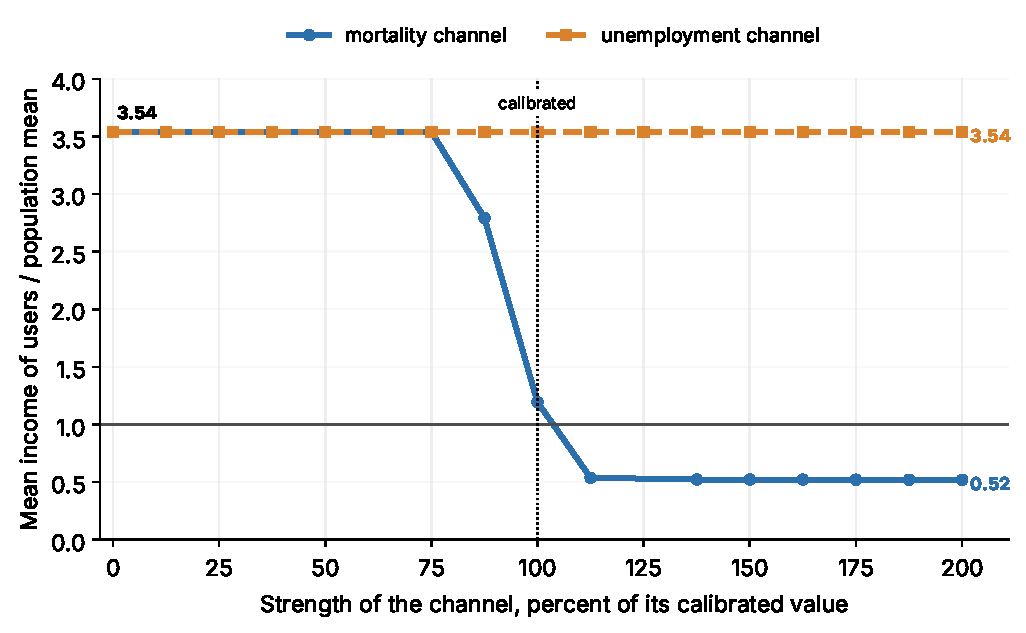
\includegraphics[width=0.62\textwidth]{figures/stylized_who_uses.pdf}
\caption{What it takes to reverse the income gradient in drug use}
\label{fig:who}
\notes{0.62\textwidth}{Notes: stage 1, the model without the child. Each curve
scales one channel with the other switched off, so both start from the economy with no
consequences of a SUD. The vertical axis is average income of users over the
population average, and $b$ is recalibrated at every point so that participation is
the calibrated $@@s1_part_ref@@$ percent. The black dotted line marks the calibrated strength; everything to
the right of it is extrapolation.}
\end{figure}

On its own,
the mortality channel takes the income ratio from @@s1_r_none@@ with nothing switched on
down to @@s1_r_mortonly@@ at its calibrated strength, and @@s1_r_mort_hi_dir@@
@@s1_r_mort_hi@@ as it continues to rise to $@@s1_scanhi_pc@@$ percent of its calibrated
value. With both channels at their calibrated strength the ratio is @@s1_r_cal@@: the unemployment channel, which does nothing on its own, adds to the mortality channel once it is in place. 
What mortality destroys is a continuation value,
and a household only stops using when the expected loss of that value exceeds what
the drug is worth to it.

In contrast, the unemployment channel does not reverse the gradient at all: on its
own it leaves users at @@s1_r_jobonly@@ times average income at its calibrated strength,
against @@s1_r_none@@ with nothing switched on, and at $@@s1_scanhi_pc@@$ percent they
are still at @@s1_r_unemp_hi@@. A resource penalty does not produce the concentration of
drug use at the bottom.

Why should the two channels differ at all, when both punish the household? Because the cost of only one of them rises quickly enough with the household's income. Who uses is decided by a race between two things that change with income. On one side is the utility cost of the drug: a household with a higher income gives up less marginal utility for each dollar it spends on drugs, so buying $v$ units costs a rich household little in terms of utility relative to a poor household.

On the other side are the expected penalties from acquiring a SUD. The unemployment penalty cannot offset the falling utility price of the drug, because it does not rise with income. A job the disorder costs is not
covered by UI, but the household can save, and savings grow with income, so a richer household that loses its job to a SUD keeps about the same share of its resources as a poorer one. Since losing the same share costs a rich household no more in utility terms than a poor one, the penalty weighs on the rich no more than on the poor. Raising it reduces use, but once $b$ brings the drug use rate back to its target, the drug is still cheapest for the rich and use stays at the top.

Mortality is a different object. Dying is a disproportionate loss that cannot be mitigated through insurance. It destroys the whole
continuation value: the consumption of a life still to be lived, and $\aleph$,
the value of being alive at all, which no amount of savings can protect. A richer household, therefore, has more to lose by dying, resulting in an expected penalty to using that rises with income. This means that once income is high enough the cost outweighs what the drug is worth to the household, and at that point it is the rich who stop first.

%======================================================================
\subsection{How does housing assistance shape the \texorpdfstring{drug-use}{drug-use} decision?}\label{sec:mh}

The two forces of question 2, moral hazard and the value of life, can be separated exactly, because they differ in
what happens to a household that uses. Under Treatment First the voucher is
withdrawn from any household that violates the sobriety condition, so only the
value-of-life force operates. Under Housing First a voucher is not revoked for sobriety-related reasons, so both the moral-hazard and the value-of-life forces operate. Comparing the two policies at the same generosity therefore isolates
the moral-hazard force, and comparing Treatment First with no programme at all
isolates the value-of-life force.

Panels A and B of Table~\ref{tab:stage1} put numbers on both, in the baseline of stage 1. With no
programme at all, $@@s1_part_none_b@@$ percent of households use. Treatment First takes that down to $@@s1_part_tf_b@@$ percent, which means that the value-of-life force reduces drug use by $@@s1_vol_b_abs@@$ percentage points.
Switching to Housing First then raises it @@s1_hf_vs_none@@, to
$@@s1_part_hf_b@@$ percent, so the moral-hazard force raises drug use by $@@s1_mh_b@@$
percentage points and the
net effect of both forces under Housing First is a $@@s1_net_b_abs@@$ percentage-point @@s1_net_dir@@ in drug use relative to
no vouchers at all.\footnote{The SUD rate follows participation one for one, since every user runs the same risk: $@@s1_sud_none_b@@$ percent of households have the disorder with no programme, $@@s1_sud_tf_b@@$ under Treatment First and $@@s1_sud_hf_b@@$ under Housing First. Homelessness falls under both programmes, from $@@s1_homeless_none_b@@$ percent to $@@s1_homeless_tf_b@@$ under Treatment First and to $@@s1_homeless_hf_b@@$ under Housing First.} Both comparisons here are between long-run steady states, each the rest point of
the economy under a policy that has always been in place. Both forces are
first order and they work against each other, which is the central feature of
the problem. The point of this analysis, beyond showing how to isolate these forces, is to illustrate that anyone asserting that housing the homeless must increase drug use,
or must reduce it, is making a quantitative claim that needs to be tested.

\begin{table}[!tb]
\centering
\caption{Stage 1: the two forces and the welfare of conditionality}\label{tab:stage1}
\sbox{\ntbox}{% Generated by code/stylized/stage_results.py from stage 1.
\footnotesize
\begin{tabular}{@{}lccc@{}}
\toprule
 & \textcolor{red}{None} & \textcolor{red}{TF} & \textcolor{red}{HF} \\
\midrule
\multicolumn{4}{@{}l}{\emph{Panel A. Outcomes, percent of households}} \\
\textcolor{red}{\quad Drug participation} & \textcolor{red}{9.49} & \textcolor{red}{1.53} & \textcolor{red}{9.02} \\
\textcolor{red}{\quad Carrying a SUD} & \textcolor{red}{3.925} & \textcolor{red}{0.632} & \textcolor{red}{3.729} \\
\textcolor{red}{\quad Homeless} & \textcolor{red}{1.378} & \textcolor{red}{0.998} & \textcolor{red}{1.014} \\
\addlinespace
\multicolumn{4}{@{}l}{\emph{Panel B. The two forces on participation, percentage points}} \\
\textcolor{red}{\quad Value of life, TF less none} &  & \textcolor{red}{$-7.96$} &  \\
\textcolor{red}{\quad Moral hazard, HF less TF} &  &  & \textcolor{red}{7.49} \\
\addlinespace
\multicolumn{4}{@{}l}{\emph{Panel C. Treatment First against Housing First}} \\
\textcolor{red}{\quad Households strictly worse off, percent} &  & \textcolor{red}{8.0} &  \\
\textcolor{red}{\quad Households strictly better off, percent} &  & \textcolor{red}{0.0} &  \\
\textcolor{red}{\quad CEV of those affected, percent} &  & \textcolor{red}{$-0.51$} &  \\
\textcolor{red}{\quad CEV of the population, percent} &  & \textcolor{red}{$-0.040$} &  \\
\bottomrule
\end{tabular}
}\usebox{\ntbox}
\tabnote{Notes: stage 1, the model without the child and without the disamenity of
homelessness. None is no programme. Welfare changes are consumption-equivalent
variations (CEV): the proportional change in consumption, in every period and state, worth
as much as the difference in lifetime value, negative when Treatment First reduces welfare relative to
Housing First.}
\end{table}

%======================================================================
\subsection{Welfare}\label{sec:welfare}

\subsubsection{Without externalities, Housing First always wins}\label{sec:nox}

Sections~\ref{sec:who} and~\ref{sec:mh} established what each policy does to
behaviour. This section asks what each does to welfare, comparing the two with the same $\pi_V$ and $p_v$, in the baseline of stage 1, where nothing a household does
affects anyone else. Welfare is measured throughout as a consumption-equivalent
variation (CEV), set out formally in Section~\ref{sec:cev}. The policies differ only in the last indicator in
equation~\eqref{eq:vouch}, so Housing First transfers resources in a superset of
the states in which Treatment First does. The budget set is weakly larger in
every state and strictly larger in one, so a rational household with no commitment problems cannot be
worse off under Housing First:
\begin{equation}\label{eq:dom}
V_1(y;\ \text{Housing First},\ \pi_V) \;\ge\; V_1(y;\ \text{Treatment First},\ \pi_V)
\qquad \text{for every } y,
\end{equation}
with equality exactly for households that would not use under Housing First for any combination of unemployment and voucher draws they may receive in period 1. Put the other way round, a
household under Housing First can reproduce its Treatment First outcome exactly
by not using: conditionality removes an option from a forward-looking optimiser
and gives nothing back. This is a dominance argument, not a calibrated result,
and no choice of parameters overturns it.

It follows that the moral hazard is not an inefficiency. Households here face the
true SUD hazard and make no mistakes, so the extra use Housing First
induces is not a wedge to be closed but a household taking a risk it rationally chooses to bear. The moral-hazard force of Section~\ref{sec:mh} is a
statement about drug use and not about welfare.

Panel C of Table~\ref{tab:stage1} puts welfare numbers on it: $@@s1_worse_b@@$ percent of households are strictly worse off under
Treatment First,\footnote{The share worse off is @@s1_worse_vs_part@@ the $@@s1_part_hf_b@@$
percent who use under Housing First. Welfare is measured before a household learns its period 1 unemployment and voucher draws. Take a household with a given productivity that would use only after a certain combination of draws, for example only if it lost its job. Before the draws, it is worse off under Treatment First, because it may end up in that combination, but it counts among the users only in the cases in which it does. A household that would not use under any combination is not worse off.} none is better off, and those affected lose the equivalent of $@@s1_cevaff_b@@$ percent
of consumption. Those are the households that would use under Housing First after some combination of draws, and so could lose a voucher under Treatment First, in period 1 or, if they acquire a SUD, in period 2. A household that would never use, regardless of its unemployment and voucher draws, is indifferent to which programme is in place. 

Therefore, the case for conditionality in
this model has to come from elsewhere: from what a household's drug use does to
somebody else.\footnote{Spending what Treatment First saves on a higher $\pi_V$, so that the two programmes cost the same, raises $\pi_V$ by only $@@s1_bb_pv_pc@@$ percent. That makes $@@s1_bb_better@@$ percent of households that never use and may draw a voucher slightly better off, but those that would use under Housing First still lose, and on average households would still give up $@@s1_bb_cevpop@@$ percent of consumption to keep Housing First, about @@s1_bb_frac@@ of the $@@s1_cevpop_b@@$ percent at the same $\pi_V$ as in the benchmark of stage 1.}

%======================================================================
\subsection{Stage 2: the child}\label{sec:kids}

Up until this point, I have shown that without externalities, and at fixed prices and access to vouchers, Housing First weakly dominates Treatment First. From a model point of view, stage 1 assumed that the child only appeared as an adult: nothing its parent did affected it, and nobody counted it before then. This stage adds the child and, with it, the externalities, and then refits the model with the child in place.

\paragraph{The child in the household.} Each household raises one child
during its adulthood period. The child shares the household's consumption and housing
through the equivalence scale $\xi$, while the drug only enters the utility of the parent, so the parent and the child hold different bundles,
\begin{equation}\label{eq:bundleskid}
X_P=\Big[\Big(\frac{c}{\xi}\Big)^{1-\gamma}\Big(\frac{h}{\xi}\Big)^{\gamma}\Big]^{1-\theta}(b+v)^{\theta},
\qquad
X_c=\Big[\Big(\frac{c}{\xi}\Big)^{1-\gamma}\Big(\frac{h}{\xi}\Big)^{\gamma}\Big]^{1-\theta}\,b^{\theta},
\end{equation}
where $X_P$ denotes the parent's bundle and $X_c$ the child's, and the parent's flow utility in period 1 is
\begin{equation}\label{eq:ukid}
u_1(c,h,v) \;=\; U(X_P)\;+\;\omega_c\,(\xi-1)\,U(X_c)\;+\;\aleph .
\end{equation}
The child consumes the household's consumption and housing but none of the drug, so
a parent's drug spending reaches it only by taking consumption and housing out of what
they share, and it counts as $\xi-1$ of the household against the scale. The weight $\omega_c$ is the
share of the child's utility that the parent takes into account. Without the drug and with
$\omega_c=1$, the first two terms become $\xi\,U(X)$, which
counts the household as $\xi$ adult equivalents: the parent as one and the child as the
remaining $\xi-1$. In period 2, when the parent moves into old age, the child leaves and the parent lives alone, meaning that $\xi=1$, and flow utility is that of~\eqref{eq:u}.

\paragraph{The child leaves.} At the end of period 1 the child leaves the
household and becomes an adult, entering period 1 of its own adulthood, with its own child living with it. Its productivity
is correlated with its parent's, and it is further permanently reduced if the parent acquired the disorder while the
child lived with it,
\begin{equation}\label{eq:kids}
\log y_{\text{child}} \;=\; \rho\log y+(1-\rho)\mu_y+\varepsilon
-\delta_d\,\mathbf{1}\{d'=1\},
\qquad \varepsilon\sim\mathcal N\big(0,\,(1-\rho^2)\,\sigma_y^2\big),
\end{equation}
where $\rho$ is the persistence of productivity across generations, $\mu_y=-\sigma_y^2/2$ is the mean of log productivity, which keeps its centre and the variance of $\varepsilon$ its spread the same
in every generation, and $\delta_d$ is the earnings penalty for the parent's disorder.\footnote{The penalty runs through income rather than through anything the child inherits about the drug. Letting the child inherit a greater susceptibility, a higher $\pi_d$, would be inconsistent with the data: a child facing a higher chance of converting use into a SUD optimally uses \emph{less} ex ante, while children of parents with a SUD are \emph{more} likely to use, not less. Income works on both counts, and it works through the channels explored in Section~\ref{sec:who}: lower permanent income is unambiguously bad to receive, and this model already puts users at the bottom, so a child born poorer is mechanically more likely to use, which is aligned with the data. It is also supported by the empirical evidence reviewed in Section~\ref{sec:literature}. The income gradient does the whole job, so the model transmits a SUD across generations without the child inheriting any greater susceptibility to the disorder.} 

\paragraph{The parent's problem.} The child enters the parent's problem
twice, once for each part of its life. In childhood it is the second term
of~\eqref{eq:ukid}. As an adult it is the continuation value $D(y,d')$, which measures what the parent's disorder costs their child in the child's own lifetime value,
\begin{equation}\label{eq:damage}
D(y,d')\;=\;\mathbb{E}\big[\bar V_1(y_{\text{child}})\,\big|\,y,\,0\big]
-\mathbb{E}\big[\bar V_1(y_{\text{child}})\,\big|\,y,\,d'\big]\;\ge\;0,
\end{equation}
where $\bar V_1$ is the value of entering period 1, before its draws, at the child's
productivity from~\eqref{eq:kids}. The first term is for a parent without the disorder and the second for the parent's own $d'$. So $D(y,0)=0$, and the loss is $D(y,1)$ when the parent's use leads to the disorder. $D(y,d')$ captures the direct impact of the parent's SUD on their child's utility, which runs through the child's earnings. It enters as a difference and not
a level, so it costs the parent nothing unless their use makes the disorder possible. The parent's period-1 problem in~\eqref{eq:v1} in Section~\ref{sec:problem} then becomes
\begin{equation}\label{eq:v1kid}
V_1(y,e,\eta) = \max_{\{k,\,v \ge 0,\,a' \ge 0\}}
\Big\{ u_1(c,h_k,v)
+ \beta\, \mathbb{E}_{d'}\Big[\phi(d')\,V_2(a',y,d')\Big]
-\ \beta\,\omega_c\,\mathbb{E}_{d'}\big[D(y,d')\big] \Big\}.
\end{equation}
$\omega_c$ multiplies both child terms. A planner who counted the child
fully would put a weight of one on both, so what the parent leaves out, $1-\omega_c$ of
the child's terms, is the externality on the child. The expectation weights $D(y,1)$ by $\pi(v)$, the chance that the use turns into a disorder. $V_1$ depends on $D$ through the
parent's problem and $D$ on $V_1$ through the child's problem, so the two are solved as a
fixed point.

\paragraph{Calibrating the child.} With the child added, $\xi$, $\rho$, $\delta_d$ and
$\omega_c$ need to be calibrated as well. I set $\xi$ to $\sqrt2$, the square-root scale for a household of two (OECD, 2013). The
persistence of productivity across generations, $\rho$, is set to $@@s_rho@@$, within the range of the
intergenerational elasticities of earnings in Section~\ref{sec:literature}. The penalty
$\delta_d$ is assigned the value $@@s_deltad@@$ in logs to give the $@@s_deltad_pc@@$-percent earnings loss Nilsson (2017)
measures for children exposed in utero to a temporary Swedish policy that let grocery
stores in two regions sell strong beer, which made alcohol easier to buy during pregnancy.
The parent's weight on their child $\omega_c$ is fitted so that switching the child's terms
off, with every other parameter held, raises the share who use drugs by $@@s_t_gap@@$ percent. Switching the terms off keeps the household as it is and removes only the parent's concern for the child, so its counterpart in the data holds the household fixed too: in NSDUH 2024, an unmarried adult living with one other adult and no child was $@@s_t_gap@@$ percent more likely to use drugs than a lone parent living with one child, both unmarried and of the same age, sex and family income (Section~\ref{sec:fullcal}). Every other stage 1 parameter is refitted with the child in place, and
Table~\ref{tab:int} reports both.


\paragraph{Treatment First with the child counted.} Counting the child's utility in
welfare, as Section~\ref{sec:cev} describes, a newborn is better off in the long run under Treatment First than under Housing First, by $@@s2_cev_tf@@$ percent of lifetime consumption. Treatment First cuts participation from $@@s2_part_hf@@$ to $@@s2_part_tf@@$
percent and the share with the disorder from $@@s2_sud_hf@@$ to $@@s2_sud_tf@@$
percent, both at each policy's rest point, so fewer children enter adult life with the penalty. Breaking the gains by periods of life shows @@s2_split@@: the gain is $@@s2_cev_tf_kid@@$ percent in childhood, because parents spend more of their
resources on them instead of on drugs, and $@@s2_cev_tf_adult@@$ percent in adult life, because the child enters with a better productivity draw. Treatment First @@s2_homeless_dir@@
homelessness too, by about $@@s2_homeless_chg_pc@@$ percent, because fewer households have a SUD and lose their jobs, and fewer are themselves poor for having been born to a
parent with the disorder, so their income is higher.

%======================================================================
\subsection{The transition}\label{sec:trans}

Comparing rest points hides a key tradeoff. Normally, the debate sees Treatment First as taking immediately and
giving back only later. In this model, this happens too: at implementation a household with a SUD can do nothing about
its condition but loses its voucher, and it is then at a higher risk of homelessness,
whereas lower substance use pays off only for the
generations after it. However, in the stylized model, a reduction in drug use actually benefits children even upon impact, and no child is worse off while living at home: children live with their parents only before the parents can have a SUD, so a parent can still respond to the reform by stopping, and their child then escapes the earnings penalty and consumes more at home. In the full model, children do live with parents who have a SUD, and indeed some children are worse off and some become homeless, but most children benefit and on net the gain is large.

The reform moves the programme from Housing First to Treatment First at the same
$\pi_V=@@s_pv@@$, in the model with the child, and every generation alive
when it lands is counted, each over its own remaining life and against what the old
rule would have given it. Figure~\ref{fig:trans} shows the paths for drug use, the disorder and homelessness of each generation as adults, from the adults at the reform on, against the Housing First rest point. It also shows the welfare of every generation: the old and the adults alive at the reform, their children, and the cohorts born after them.

The old, in their second period, chose under the old rule,
carry whatever disorder that choice left them and cannot recover in a terminal period;
conditionality now revokes the voucher from income-eligible households with a SUD that happened to draw one, and they lose
$@@s4_tr_old_abs@@$ percent of consumption, with $@@s4_tr_old_hl_tf@@$ percent of them
homeless against $@@s4_tr_old_hl_hf@@$ under the old rule. The adults, in their first
period with their children at home, who were born into the old distribution, choose
under the new rule; they lose $@@s4_tr_young_abs@@$ percent over their adult lives, which is the price of an option removed.

Their children, the first cohort born into the reform, gain
$@@s4_tr_c1@@$ percent: $@@s4_tr_c1_adult@@$ in adult life, since they are the first to
enter it with the draws of parents who chose under Treatment First, and $@@s4_tr_c1_kid@@$ in childhood, against the
$@@s4_tr_c2_kid@@$ that childhood contributes in the long run, since the parents they grow up with were themselves born
into the penalised distribution. From the second cohort on the chain is at its
new rest point and every cohort gains the long-run $@@s4_tr_c2@@$ percent. The cost
falls on the adults and the old alive at the reform, and the benefit on the children
born at the reform and, @@s4_tr_more@@, on every cohort born after them.

\begin{figure}[!tb]
\centering
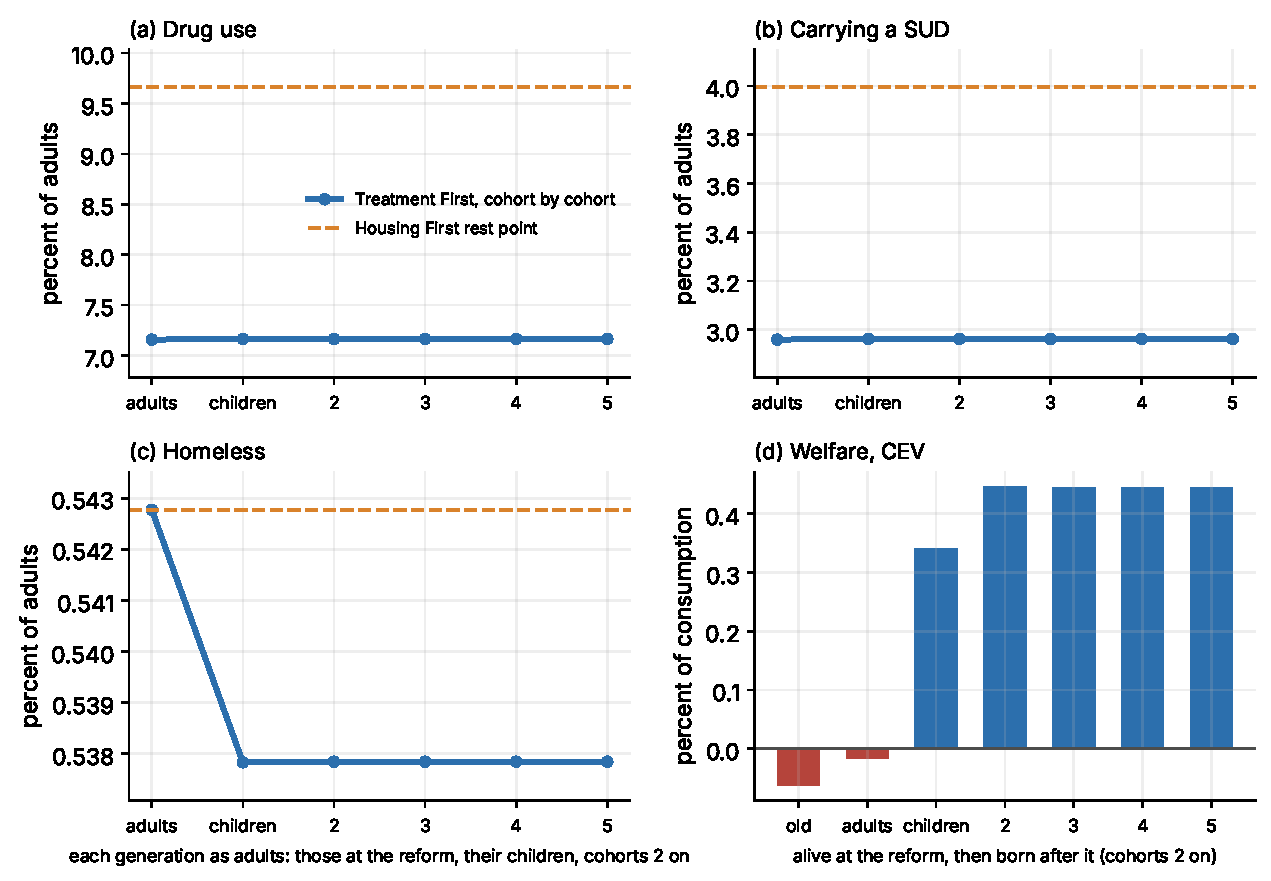
\includegraphics[width=\textwidth]{figures/stylized_transition.pdf}
\caption{The transition from Housing First to Treatment First}\label{fig:trans}
\notes{\textwidth}{Notes: the model with the child. Panels (a) to (c) are each
generation as adults, in their first period: the adults at the reform, who were born into
the Housing First distribution and choose under Treatment First, their children, and the
cohorts born after them, when they become adults, to the @@s4_tr_n_ord@@; the solid blue line is Treatment First,
cohort by cohort, and the dashed orange line is the Housing First rest point. Panel (d)
is each generation's CEV against Housing First: the old and the adults alive at the
reform over the rest of their lives, and their children and every cohort born after them
over their whole lives.}
\end{figure}

%======================================================================
\subsection{Stage 3: the disamenity of homelessness}\label{sec:kx}

Before moving onto the full model, I take up the aggregate homelessness externality. The externality is modelled such that homelessness imposes a cost on each household's flow utility, reducing it by $\kappa_x H$, where $H$ is the share of households that is homeless, which every
household takes as given, so the term moves no choice and the calibration of stage 2
stands unchanged. It enters welfare only, and the child
bears it like everyone else, once for each period.

$\kappa_x$ is solved inside the model from the annual willingness to pay for ending homelessness in the contingent valuation of Loubi\`ere et al.\ (2020), $@@s3_wtp_pc@@$
percent of income. Households in the model spend $@@s3_cshare_pc@@$ percent of their income
on consumption, so $@@s3_wtp_pc@@$ percent of income translates to $@@s3_wtp_c_pc@@$ percent of consumption. $\kappa_x$ is the
disamenity per unit of homelessness, in utils per period alive, that costs an adult in
the stage 2 economy as much over its adult life as giving up $@@s3_wtp_c_pc@@$ percent of
its consumption in every period.\footnote{\label{fn:kx}$\kappa_x$ solves
$V\big((1-w)\,c;\,0\big)=V\big(c;\,H\big)$, where $V(c;H)$ is an adult's lifetime value in
the stage 2 economy when it consumes $c$ and homelessness is $H$, which it bears as the disamenity
$\kappa_x H$, and $w$ is the
willingness to pay as a share of consumption to have $H=0$.} That gives
$\kappa_x=@@s3_kx@@$. Because the two policies differ little in homelessness, @@s3_kx_phrase@@
$@@s3_cev_tf@@$ percent of lifetime consumption.

%======================================================================
\section{The quantitative model}\label{sec:full}

By now, I have shown how the main mechanisms in this paper work. This section
describes the model the paper's numbers come from. It is very similar to the stylized
model of Section~\ref{sec:stylized}, but includes annual periods and pieces that model leaves out: income risk during working age, retirement, progressive income taxes, interest on savings, a drug-use decision in every year, recovery, relapse and treatment, SMI, a higher risk of dying, worse employment prospects and a lower chance of recovering while homeless, children who can live with a parent who has a SUD, a drug test that misses some users, a balanced government budget and an endogenous drug price. Notation follows
Section~\ref{sec:stylized} wherever the two models share an object: $\gamma$ and
$\theta$ are the housing and drug weights in both, $\sigma$ the same risk aversion, $b$ is
the same Stone-Geary shifter, $\aleph$ the same flow value of being alive, $\xi$ the same equivalence
scale, $\omega_c$ the same weight on the child, $\rho$ and $\delta_d$ the same
persistence of productivity and penalty, $\psi_{ui}$ and $\bar y$ the same replacement
rate and earnings cap, $\kappa_x$ the same disamenity, $\pi_d$ the same chance that use
starts a SUD, $\kappa_{\phi d}$ the same mortality multiplier for the disorder, $h_1$ the same
shelter, $\kappa_V$ and $\pi_V$ the same means test and chance of drawing a voucher, $p_r$ the
same rent, and $\beta$ is the same discount factor.  The values are in Section~\ref{sec:fullcal}.

\subsection{Demographics and the state and choice sets}

Households enter the economy as adults at model age $j=1$, live
at most $J$ annual periods, work while $j<J_R$ and are retired from $J_R$. Each has a
child, who lives in the household for the first $J_K$ years of its adult life and then
leaves to become an adult with a child of its own. Each period a cohort of unit mass enters at $j=1$, made up of
the children who leave home that period, at their parent's death if that comes before $J_K$ and at $J_K$
otherwise (equation~\eqref{eq:flomnew}), so the mass of households is constant in a stationary equilibrium. The individual state is age $j$ together with
\begin{equation}\label{eq:fstate}
s=(a,\,y,\,e,\,d,\,m,\,\eta)\in
\mathbb R_+\times\mathcal Y_j\times\{1,2,3\}\times\{0,1,2\}\times\{0,1\}\times\{0,1,2\},
\end{equation}
where $a$ denotes assets, $y$ productivity, $e$ employment status, $d$ the SUD, $m$
SMI and $\eta$ the household's standing with the voucher programme. The SUD takes
three values because the parent's valuation of their child's prospects depends on their history and not only on its present (Section~\ref{sec:fproblem}): $d=0$ denotes a household that has never carried the disorder, $d=1$ refers to
one that carried it and has recovered, and $d=2$ stands for one that carries it now. The
voucher state is $\eta=0$, denoting having no voucher, $\eta=1$, representing
holding one, and $\eta=2$, standing for exclusion from the programme after failing
Treatment First's condition.

Each period the household chooses the bundle
\begin{equation}\label{eq:fchoice}
\big(h,\,v,\,\tau,\,a'\big)\in
\{h_1,h_2,h_3,h_4\}\times\mathbb R_+\times\{0,1\}\times\mathbb R_+ ,
\end{equation}
where $h$ is the dwelling, of which $h_1$ is a shelter, $v$ is drug consumption, $\tau$ is whether or not a household is in treatment for SUD, available only to a household that has
the disorder, and $a'$ is its next period's assets. Labour is inelastically supplied when employed.

\subsection{Preferences}\label{sec:fprefs}

Flow utility is the stylized model's, with the child present for the first $J_K$
years. Consumption $c$ and housing $h$ are shared through the equivalence scale $\xi_j$, which scales for two members while the child is at home and for one
after, and the drug enters the parent's utility alone, so the parent and the child hold the bundles
\begin{equation}\label{eq:fbundles}
X_P=\Big[\Big(\frac{c}{\xi_j}\Big)^{1-\gamma}\Big(\frac{h}{\xi_j}\Big)^{\gamma}\Big]^{1-\theta}(b+v)^{\theta},
\qquad
X_c=\Big[\Big(\frac{c}{\xi_j}\Big)^{1-\gamma}\Big(\frac{h}{\xi_j}\Big)^{\gamma}\Big]^{1-\theta}b^{\theta},
\end{equation}
and period utility is
\begin{equation}\label{eq:futil}
u\big(c,h,v,\tau\big) \;=\; U(X_P)\;+\;\omega_c\,(\xi_j-1)\,U(X_c)\;+\;\aleph\;-\;\tau\,\bar\tau^{u}\;-\;\kappa_x H,
\qquad U(X)=\frac{X^{1-\sigma}}{1-\sigma}.
\end{equation}
$\gamma$ is housing's share of the non-drug bundle and $\theta$ the drug's share of
the whole, $\sigma$ is the coefficient of relative risk aversion, $\aleph$ is a flow value of being alive, counted once per household, and $\bar\tau^{u}$ is the utility
cost of a year in treatment, which is described in Section~\ref{sec:fdrug}. The child's term is its own flow utility, which the parent weighs by $\omega_c$, and is counted as $\xi_j-1$ of the household; it gets none of the drug, so a parent's drug spending reaches it through a reduction in the consumption and housing they share. After $J_K$ periods the child leaves to form its own household, and the child term is gone, at which point $\xi_j=1$ for the parent.

Aggregate homelessness $H$ carries the disamenity $\kappa_x H$ for every household and
child alive, which is what makes homelessness an externality for everyone rather than only a
private misfortune. However, it does not affect any household's decision: each takes $H$ as given.
Section~\ref{sec:fleftout} takes up its size.

\subsection{Income, taxes and transfers}\label{sec:ftaxes}

\paragraph{Productivity.} Log productivity follows a persistent process over
working life, $z_{j+1}=\rho_z z_j+\zeta_{j+1}$ with $\zeta\sim\mathcal N(0,\sigma_\zeta^2)$, and is held fixed at its last working value in retirement. Earnings on the job are
$y\,\varepsilon(j)$, with $y=e^{z}$ normalised so that $y$ averages one at
entry and $\varepsilon(j)$ the deterministic age profile. A
household's productivity at entry is its inheritance from its parent, set out in
Section~\ref{sec:fnewbornsec}; its spread combines $\sigma_\zeta$ with a persistent
component drawn at entry, and a child entering with the penalty of that section is on a
separate block of the grid, with the base grid scaled down for life.

\paragraph{Before-tax income.} Before-tax income depends on age and employment,
\begin{equation}\label{eq:fincome}
Y(j,y,e)=
\begin{cases}
y\,\varepsilon(j) & j<J_{R},\ e=1 \quad\text{(employed)}\\[2pt]
\psi_{ui}\,\min\{y\,\varepsilon(j),\ \bar y\} & j<J_{R},\ e=2 \quad\text{(insured, first year out of work)}\\[2pt]
0 & j<J_{R},\ e=3 \quad\text{(out of work, uninsured)}\\[2pt]
S(y) & j\ge J_{R} \quad\text{(retired)} .
\end{cases}
\end{equation}
UI replaces a share $\psi_{ui}$ of earnings on a base capped
at $\bar y$, and it is paid only to a share $p_{ui}$ of those losing their job, mimicking the share of
insured separations. After the first year, unemployed households, insured and uninsured alike, receive
zero UI ($e=3$). Social security $S(y)$ follows the statutory formula.\footnote{\label{fn:ss}Let $\tilde y=\min\{y,\,y^{\max}\}$ denote the household's productivity at its last
working age up to the taxable maximum $y^{\max}$, the ceiling above which earnings no longer raise the benefit. Then social security payments are $S(y)=\bar w\max\big\{\underline S,\ \alpha_1\min\{\tilde y,k_1\}+\alpha_2\max\{0,\min\{\tilde y,k_2\}-k_1\}
+\alpha_3\max\{0,\tilde y-k_2\}\big\}$, where $k_1<k_2$ are the two bend points,
$\alpha_1>\alpha_2>\alpha_3$ the shares replaced below, between and above them,
$\underline S$ the Supplemental Security Income (SSI) payment, and $\bar w$ the benchmark's average labour income. Their values are given in Appendix~\ref{sec:stdparams}.}

The SUD and SMI do not
cut earnings on the job; they act on whether there is a job at all, through the
employment transitions below. Out of work, a household with the SUD or SMI is paid what any other household is:
UI in its first year with probability $p_{ui}$, nothing with probability $1-p_{ui}$, and
nothing after the first year. There is no
disability insurance in the model, so SMI brings no income of its own.\footnote{In the
data only a minority of adults with SMI receive disability benefits on the basis of a mental
disorder: about 3 million, through Social Security Disability Insurance or SSI, against 14.6
million adults with SMI in NSDUH 2023, roughly one in five.}

\paragraph{Taxes.} Before-tax income is taxed with the Heathcote et al.\ (2017) function
and capital income at a flat rate, so that after-tax income is
\begin{equation}\label{eq:ftax}
y^{n}=\min\big\{Y,\ \tau_{\ell}\,Y^{\varphi}\big\}\;+\;(1-\tau_k)\,r\,a ,
\end{equation}
where $\tau_{\ell}$ scales after-tax income, and so sets the level of the tax, which falls as $\tau_{\ell}$ rises, and $1-\varphi$ sets
its progressivity; $\tau_k$ is the flat tax rate on capital income and $r$ is the exogenous interest rate on savings.\footnote{The minimum keeps the labour income tax from turning negative, since at low incomes $\tau_{\ell}Y^{\varphi}$ exceeds $Y$ itself.}

\paragraph{Transfers.} Food assistance pays the maximum allotment $\underline c$ less
the share $\varrho$ of income, and the voucher pays a holder that is eligible this
period the rent on the dwelling above a tenant contribution of $\kappa_r$ of income, up
to the fair market rent ($\mathit{FMR}$),
\begin{equation}\label{eq:ftrans}
\begin{aligned}
F&=\max\big\{0,\ \underline c-\varrho\,\hat y\big\},\\
V\!ch&=\mathbf{1}\{\eta=1\}\,\mathbf{1}\{\hat y<\kappa_V y^{\text{med}}\}\,\mathbf{1}\{h\neq h_1\}\,
\min\Big\{\max\{0,\ p_r h-\kappa_r\hat y\},\ \max\{0,\ \mathit{FMR}-\kappa_r\hat y\}\Big\},
\end{aligned}
\end{equation}
where $\hat y=Y+ra$ is the income both programmes are means-tested on,
$\kappa_V$ and median income $y^{\text{med}}$ are the eligibility rule
in Section~\ref{sec:fvoucher}, and $\mathit{FMR}$ is the average rent paid by housed households in
the benchmark. A voucher
holder in a shelter keeps the voucher and is paid nothing until it rents again, as long as it keeps its eligibility. Voucher holders
keep their vouchers for as long as they remain eligible. Each
entering household receives a one-time endowment $T_0$ from bequests left by deceased households, and the
government collects the rest of the estates of the dead.

\subsection{The budget constraint}

The household's budget constraint is as follows:
\begin{equation}\label{eq:fbudget}
c+p_v v+a' \;=\; y^{n}+a+T_0\mathbf{1}\{j=1\}\;-\;p_r\, h\,\mathbf{1}\{h\neq h_1\}\;+\;V\!ch+F,
\qquad c\ge F,\ v\ge0,\ a'\ge0 .
\end{equation}
Food assistance is paid in kind, so it cannot directly fund the drug, the rent or saving. The
drug price is $p_v$, which is endogenous here as opposed to exogenous like in the
stylized model, and the rent per unit of housing $p_r$ is fixed and held at its benchmark value
in every simulation. Treatment costs utility only.

\subsection{Housing and the homelessness loop}

Housing is the four-point grid of~\eqref{eq:fchoice}: $h_1$ is literal
homelessness, sleeping rough or in an emergency shelter, which is free, and $h_2<h_3<h_4$
are three rental sizes.

Homelessness then enters three separate equations: survival~\eqref{eq:fsurv} and the
employment transitions~\eqref{eq:femp}, both in Section~\ref{sec:fcosts}, and the SUD recovery hazard~\eqref{eq:frecover} in Section~\ref{sec:fdrug}.
It raises mortality, worsens both employment margins and lowers the chance of
recovering from the SUD. SMI is the one thing it does not reach, for the reason given
in Section~\ref{sec:fsmi}.

\subsection{Drug use, the SUD, recovery and treatment}\label{sec:fdrug}

A household that does not have the disorder, either $d=0$ (never had it) or $d=1$ (had it
but recovered), and uses acquires it ($d=2$) with probability $\pi_d$,
\begin{equation}\label{eq:fd}
\Pr(d'=2\mid d\neq 2,\,v)=\pi_d\,\mathbf{1}\{v>0\},
\end{equation}
and a household that has
recovered can acquire the disorder again. A household may begin using only up to an
age $J_E$.\footnote{Without it there is little-to-no consequence at old ages to using: too
little life remains for the disorder to damage, so the model produces too much of
it. The cause is that death is certain at the last age $J$, so close to it a household
knows how little life remains, whereas in real life the vast majority of people do not know exactly when they will die.
Section~\ref{sec:fullcal} gives the value of $J_E$.} A household with the SUD recovers, to $d=1$, with probability
\begin{equation}\label{eq:frecover}
\begin{aligned}
\pi_r(h,m,\tau)=\min\Big\{1,\ \bar\pi_r\,&\big(\mathbf{1}\{h=h_1\}\,\mu_H+\mathbf{1}\{h\neq h_1\}\big)\big(\mathbf{1}\{m=1\}\,\mu_m+\mathbf{1}\{m=0\}\big)\\
&\times\big(\mathbf{1}\{\tau=1\}\,g+\mathbf{1}\{\tau=0\}\big)\Big\},
\end{aligned}
\end{equation}
where $\bar\pi_r$ is the baseline annual chance of recovering while housed, without SMI and untreated. It has three multipliers on it: $\mu_H<1$, which means that recovery is
harder in a shelter, $\mu_m<1$, which means that it is harder with SMI, and $g>1$,
which means that it is more likely in treatment.

$\mu_H$ is how housing acts on SUD recovery here. Housing does not change what a household wants: flow utility
is the same function of $(c,h,v)$ housed or not. What housing changes is the chance of
getting out of the disorder once it is carried. Milby et al.\ (2005) randomised
cocaine-dependent homeless adults into arms differing in housing and measured weeks of
abstinence, so the ratio between arms identifies $\mu_H$ in the calibration.

Treatment $\tau$ is a choice, taken at the utility cost $\bar\tau^u$
in~\eqref{eq:futil}, and $g$ is the only thing it buys. It does not stop the household
using, it does not remove the excess mortality of the disorder while it lasts, and it
does not exempt the household from Treatment First's condition.

\subsection{SMI}\label{sec:fsmi}

$m$ is a two-state Markov chain representing SMI, mental illness severe enough to cause substantial functional impairment. It affects a small share of adults, whereas any
mental illness affects roughly a quarter of adults and includes mild anxiety. Onset
follows an age profile $\varsigma_m(j)$, normalised to one at age $26$ and scaled by the level
$\omega_m$, and a household that carries the SUD is $\iota>1$ times more likely to develop SMI than one that does not,
\begin{equation}\label{eq:fonset}
\Pr(m'=1\mid m=0,d)=\min\big\{1,\ \omega_m\,\varsigma_m(j)\,\big(\mathbf{1}\{d=2\}\,\iota+\mathbf{1}\{d\neq2\}\big)\big\},
\qquad
\Pr(m'=0\mid m=1)=\lambda_m .
\end{equation}
The effect of the SUD on SMI onset, $\iota>1$, runs in the direction the evidence
supports. About a quarter of those with a psychosis induced by a substance go on to develop
schizophrenia or bipolar disorder (Murrie et al., 2020). In the Danish registers, people with any SUD are more likely to develop schizophrenia than people with no SUD (Nielsen et al., 2017), and among those with schizotypal disorder a SUD makes the conversion to schizophrenia more likely (Hjorth\o j et al., 2018). A household with SMI recovers from it with the probability $\lambda_m$ each year, whatever its housing and whether or not it carries the SUD.

SMI then affects three objects: the chance of finding a job when unemployed, through~\eqref{eq:femp}, mortality, through~\eqref{eq:fsurv}, both in
Section~\ref{sec:fcosts}, and the SUD recovery hazard, through $\mu_m$
in~\eqref{eq:frecover} in Section~\ref{sec:fdrug}. It does not change the utility function or earnings on the job.

The SMI chain does \emph{not} depend on housing, and that is a finding in the data
rather than an omission. In the moderate-needs arm of the At Home / Chez Soi randomised trial, which followed $1{,}198$ homeless
adults with SMI across four cities, assignment to housing with intensive case
management had no detectable effect on symptom severity over twenty-four months (Stergiopoulos et al., 2015). 

\subsection{What the SUD, SMI, and homelessness cost}\label{sec:fcosts}

\paragraph{Death risk.}\label{sec:fdeath} Write $1-\bar\phi_j$ for the probability of dying
at age $j$ of a household that is housed and has neither the disorder nor SMI; the three
multipliers below raise it for every other household. Write
$q^{\,0}_j(h)=\min\{1,\big(\mathbf{1}\{h=h_1\}\,\kappa_{\phi H}+\mathbf{1}\{h\neq h_1\}\big)\,(1-\bar\phi_j)\}$ and
$q^{\,1}_j(h)=\min\{1,\kappa_{\phi d}\,\big(\mathbf{1}\{h=h_1\}\,\kappa_{\phi H}+\mathbf{1}\{h\neq h_1\}\big)\,(1-\bar\phi_j)\}$
for the probability without and with the disorder. The probability of dying is then
\begin{equation}\label{eq:fsurv}
1-\phi(j,h,d,m)=\min\Big\{1,\ \big(\mathbf{1}\{m=1\}\,\kappa_{\phi m}+\mathbf{1}\{m=0\}\big)\,q^{\,0}_j(h)
+\mathbf{1}\{d=2\}\big[q^{\,1}_j(h)-q^{\,0}_j(h)\big]\Big\},
\end{equation}
so $\kappa_{\phi H}{}>1$ multiplies the death probability when a household is in a shelter, $\kappa_{\phi d}{}>1$ when a household has a SUD, and $\kappa_{\phi m}>1$ the baseline risk when a household has SMI, to which the excess risk of the disorder is
added. A household without the disorder therefore dies with probability $q^{\,0}_j(h)$, or
$\min\{1,\,\kappa_{\phi m}\,q^{\,0}_j(h)\}$ with SMI, and the disorder adds the excess
$q^{\,1}_j(h)-q^{\,0}_j(h)$ on top. The disorder kills
whether or not it is being treated.\footnote{In the data, the meta-analyses of mortality among people using extramedical
opioids report overdose as the largest single contributor to the excess (Larney et al.,
2020; Degenhardt et al., 2011), and in the Centers for Disease Control and Prevention (CDC) WONDER database drug poisoning alone accounts for a large share of all deaths at
ages 25 to 44, which is the moment Section~\ref{sec:fvalid} reports the model
against.}

\paragraph{Unemployment risk.} A job is lost with probability $\pi^{eu}$ and found
with probability $\pi^{ue}$,
\begin{equation}\label{eq:femp}
\begin{aligned}
\pi^{eu}(y,h)&=\min\Big\{1,\ \bar\pi^{eu}\,\varpi(y)\,
\big(1+\mathbf{1}\{h=h_1\}\,\kappa_{H}\big)\Big\},\\
\pi^{ue}(h,d',m')&=\min\Big\{1,\ \frac{\bar\pi^{ue}\,\big(1-\mathbf{1}\{h=h_1\}\,\kappa_{H}\big)}
{\big(\mathbf{1}\{d'=2\}\,\kappa^{ue}_{d}+\mathbf{1}\{d'\neq2\}\big)\big(\mathbf{1}\{m'=1\}\,\kappa^{ue}_{m}+\mathbf{1}\{m'=0\}\big)}\Big\},
\end{aligned}
\end{equation}
with $\bar\pi^{eu}$ and $\bar\pi^{ue}$ the baseline separation and job finding rates,
$\varpi(y)$ a factor that makes separations likelier at low productivity, in line with the
unemployment rates of the education groups the productivity grid spans, and the divisors
$\kappa^{ue}_{d}$ and $\kappa^{ue}_{m}$ making one harder to find with the SUD and with
SMI. Neither the SUD nor SMI raises separations; each only reduces the chance of regaining employment. $\kappa_{H}$ does both for a household in a
shelter.

\paragraph{The child's productivity penalty.} A child whose parent had the disorder at any point while the child lived at home,
before $J_K$ or before the parent died if that came first, enters the economy with its productivity lowered
by the proportion $\delta_d$ in~\eqref{eq:fnewborn} in Section~\ref{sec:fnewbornsec}, and the penalty stays with the
child for life. The parent weighs the penalty through the weight $\omega_c$ they put on their child (Section~\ref{sec:fproblem}): using does
not pass the penalty on by itself, but it carries the chance $\pi_d$ of acquiring the disorder,
and with it the penalty. The penalty is a risk to the
parent's own objective only to the extent that $\omega_c$ is positive, so it carries an externality rather
than a pure personal cost, and it is the one risk that reaches the child after it has left home; parental unemployment reaches the child only while it is at home, through the reduction in household resources, which the parent likewise weighs
only at $\omega_c$.

\subsection{The voucher and the two policies}\label{sec:fvoucher}

A household is eligible for a voucher while its income is below the share
$\kappa_V$ of median income,
\begin{equation}\label{eq:felig}
\hat y\;<\;\kappa_V\,y^{\text{med}},
\end{equation}
with $\hat y$ the income of~\eqref{eq:ftrans}. A holder keeps its voucher while it is
eligible, so unlike Section~\ref{sec:support} the voucher is persistent rather than
redrawn each period, and an eligible household without one draws one with probability
$\pi_V$. Under Housing First that is the whole rule.

Under Treatment First the programme is conditional. A household fails the condition if
it uses or has the disorder, $v>0$ or $d=2$, whether or not it is in treatment. Income-eligible holders and income-eligible households that draw a voucher are tested, at a cost
$c_{\text{test}}$ each to the government, and one that fails is detected with probability
$p_{\text{det}}$, so unlike in Section~\ref{sec:mh}, enforcement is not perfect: with probability $1-p_{\text{det}}>0$ a household that fails the condition actually gets to keep its voucher. A detected holder keeps this period's payment
and loses the voucher from the next period; a detected applicant never receives it. Either way
the household is excluded from the voucher programme for a period of time, $\eta'=2$: it cannot draw a voucher whatever its income, and it
returns to the lottery, $\eta'=0$, with probability $\psi_x$ each year.

None of
$p_{\text{det}}$, $\psi_x$ and $c_{\text{test}}$ binds in the benchmark, where no voucher
is conditional, so all three are set with the experiment in
Section~\ref{sec:experiments} rather than in the calibration.

\subsection{The shocks, collected}\label{sec:fshocks}

Conditional on the state and the choices, the next period's state is drawn in five
transitions, which are independent given the state except that employment depends on
next period's SUD and SMI and on the dwelling $h$ through~\eqref{eq:femp} of
Section~\ref{sec:fcosts}:

\paragraph{Productivity $y$.} By the process of Section~\ref{sec:ftaxes} while
working, and unchanged in retirement.

\paragraph{Employment $e$.} A household that loses its job is insured with probability
$p_{ui}$, for one year. With $\pi^{ue}(h,d',m')$ and $\pi^{eu}(y,h)$ from~\eqref{eq:femp},
\begin{equation}\label{eq:fetrans}
e=1\ \longrightarrow
\begin{cases}
e'=1 & \text{w.p. } 1-\pi^{eu}(y,h)\\
e'=2 & \text{w.p. } p_{ui}\,\pi^{eu}(y,h)\\
e'=3 & \text{w.p. } (1-p_{ui})\,\pi^{eu}(y,h)
\end{cases}
\qquad
e\in\{2,3\}\ \longrightarrow
\begin{cases}
e'=1 & \text{w.p. } \pi^{ue}(h,d',m')\\
e'=3 & \text{w.p. } 1-\pi^{ue}(h,d',m').
\end{cases}
\end{equation}
State $2$ is reachable only from employment and never from itself, so the insured are
in it for the first year out of work and then move to state $3$, which pays nothing.

\paragraph{The SUD $d$.} A household without the disorder acquires it with the probability in~\eqref{eq:fd} and one with it recovers with the probability in~\eqref{eq:frecover}, both in
Section~\ref{sec:fdrug}, conditional on the chosen $v$, $h$ and $\tau$ and on $m$.

\paragraph{SMI $m$.} SMI begins and ends according to~\eqref{eq:fonset} in Section~\ref{sec:fsmi}, conditional on $d$ and age.

\paragraph{The voucher $\eta$.} A voucher is drawn and revoked according to the rule of
Section~\ref{sec:fvoucher}, conditional on this period's eligibility and, under
Treatment First, on the chosen $v$ and the state $d$.

Write $\Gamma\big(s'\mid s,\,h,v,\tau,a'\big)$ for their joint law of motion, which is
the object the expectation in~\eqref{eq:fbellman} in Section~\ref{sec:fproblem} is taken against.

\subsection{The household's dynamic problem}\label{sec:fproblem}

Putting it together, for $j=1,\dots,J$ and with $V(J{+}1,\cdot)=0$,
\begin{equation}\label{eq:fbellman}
\begin{aligned}
V(j,s)=\max_{\{h,\,v,\,\tau,\,a'\}}\ \Bigg\{\
&U(X_P)+\omega_c(\xi_j-1)\,U(X_c)+\aleph-\tau\bar\tau^{u}-\kappa_x H\\[2pt]
&+\ \beta\,\phi(j,h,d,m)\!\int_{\mathcal S}\! V(j{+}1,s')\,
\Gamma\big(\mathrm{d}s'\mid s,h,v,\tau,a'\big)\\[2pt]
&-\ \beta\,\chi_j\,\omega_c\,D(y,d)\Bigg\},
\qquad
\chi_j=\begin{cases}1-\phi(j,h,d,m) & j<J_K\\ 1 & j=J_K\\ 0 & j>J_K,\end{cases}
\end{aligned}
\end{equation}
subject to the budget~\eqref{eq:fbudget}, the income and transfer
rules~\eqref{eq:fincome} to~\eqref{eq:ftrans} in Section~\ref{sec:ftaxes}, and the restrictions that treatment is
available only to a household with $d=2$, that no household begins using after $J_E$,
and that $c\ge F$, since the food stamp payment is paid in kind and cannot be saved.

The first line is the flow of~\eqref{eq:futil}. The second is the household's own
continuation. The third is the child as an adult. It enters when the child leaves: at
$J_K$ with certainty, and before then with the probability that the parent dies first.
$D(y,d)$ is what the parent's disorder costs the child, in the child's own lifetime value,
\begin{equation}\label{eq:fchild}
D(y,d)=\mathbb{E}\big[V(1,s_{\text{child}})\,\big|\,y,\ 0\big]
-\mathbb{E}\big[V(1,s_{\text{child}})\,\big|\,y,\ d\big]\;\ge\;0,
\end{equation}
where the child is valued entering at $j=1$ with the endowment $T_0$, employed, and without the disorder, SMI or a
voucher. Its productivity is drawn as
in~\eqref{eq:fnewborn} in Section~\ref{sec:fnewbornsec} from a parent with productivity $y$. In the first term the parent has never had the disorder, and in the second they have their actual $d$, so $D(y,0)=0$. They are charged ($D(y,d)>0$ for $d\ge1$) whenever they carried the disorder at some point before the child
becomes an adult.

The term is a difference and not a level, and the
distinction is not cosmetic. Written as a level, $\omega_c$ times the child's value, it
would be worth more to a household the likelier it is to die, because it is the death
branch that carries it, and a SUD raises the death risk severalfold, so a level would
pay most to exactly the households the paper is about, for reasons that have nothing to
do with the child. Instead, when it enters as a difference, the term is zero for a parent who has never had the disorder and a cost otherwise, so what enters the decision is only the loss the parent's own history imposes on their child.

One weight $\omega_c$ multiplies both child terms, the flow of childhood and the value
of adulthood, so calibrating it pins the parent's concern for the whole of the child's
life at once. At $\omega_c=0$ the damage a household does to its child is entirely
external; at $\omega_c>0$ it internalises the share $\omega_c$ and only $1-\omega_c$
remains external. The policy functions $h(j,s)$, $v(j,s)$, $\tau(j,s)$ and $a'(j,s)$ are the dwelling, drug use, treatment and saving that solve~\eqref{eq:fbellman} at age $j$ and state $s$.

\subsection{The government}

The government pays social security, UI, food assistance
and vouchers under Housing First, with the addition of the drug tests under Treatment First. It collects the labour and capital income
taxes of~\eqref{eq:ftax} in Section~\ref{sec:ftaxes} and the estates of the dead, less the
endowment $T_0$ given to entering adults ($j=1$),
\begin{equation}\label{eq:fgovt}
\underbrace{\textstyle\sum \big(Y-\min\{Y,\tau_{\ell}Y^{\varphi}\}\big)+\tau_k\sum ra+\big(\text{estates}-T_0\big)}_{\text{revenue}}
\;-\;
\underbrace{\big(S+UI+F+V\!ch+\text{tests}\big)}_{\text{outlay}}
\;=\;\mathcal R .
\end{equation}
In the benchmark the tax parameters are set as in Section~\ref{sec:fullcal} and
$\mathcal R$ is whatever surplus they produce. In every experiment the taxes are
held at their benchmark values and the probability of drawing a voucher $\pi_V$ adjusts
so that $\mathcal R$ equals its benchmark value $\bar{\mathcal R}$.

\subsection{The drug market}

The price of the drug clears its market,
\begin{equation}\label{eq:fdrug}
p_v=\nu_1 S_v^{1/\varepsilon_s},
\qquad S_v=\sum_{j=1}^{J}\int v(j,s)\,\mathrm{d}\Phi(j,s),
\end{equation}
where $\varepsilon_s$ is the price elasticity of supply and $\nu_1$ is normalised so
that the price is one in the benchmark, and then held fixed across experiments. The
price itself is not fixed: it adjusts in every experiment to clear the drug market.

\subsection{The law of motion and newborns}\label{sec:fnewbornsec}

Given the policy functions, the distribution over states evolves by pushing
households through their choices and then through the shocks,
\begin{equation}\label{eq:flom}
\Phi(j{+}1,\mathcal S')\;=\;\int_{\mathcal S}\!\phi\big(j,h(j,s),d,m\big)\,
\Gamma\big(\mathcal S'\mid s,\,h(j,s),v(j,s),\tau(j,s),a'(j,s)\big)\,
\mathrm{d}\Phi(j,s),
\end{equation}
for $j=1,\dots,J-1$ and every measurable set $\mathcal S'$ of the state space $\mathcal S$ of~\eqref{eq:fstate}, with the integral over the state $s$ of the households of age $j$, together with the inflow of entrants
\begin{equation}\label{eq:flomnew}
\Phi(1,\mathcal S')\;=\;\frac{\sum_{j\le J_K}\int_{\mathcal S}\!\chi_j\,
\mathcal N\big(\mathcal S'\mid s\big)\,\mathrm{d}\Phi(j,s)}
{\sum_{j\le J_K}\int_{\mathcal S}\!\chi_j\,\mathrm{d}\Phi(j,s)},
\end{equation}
where the integrals are again over $s$, $\mathcal N$ places the child according
to~\eqref{eq:fnewborn} and $\chi_j$ is the weight defined in Section~\ref{sec:fproblem}. The entering cohort has unit
mass every period, so in equilibrium it equals the mass of the dead. Where an
entrant starts depends on its parent: its productivity is drawn around the parent's, and it
carries the penalty if the parent had the disorder, both as of the moment the child becomes an
adult, which is at the parent's death if that comes before $J_K$ and at $J_K$ otherwise, the
same timing with which the parent weighs its child in Section~\ref{sec:fproblem}.

An entrant starts with the endowment $T_0$, is employed, has never carried the
disorder, holds no voucher, and carries SMI with the prevalence observed at age 26.
Its log productivity is drawn around its parent's, with the persistence $\rho$ and an
innovation that keeps the spread of productivity at entry the same in every
generation, and it is scaled for life by the penalty if the parent had the disorder at any point before their child became an adult,
\begin{equation}\label{eq:fnewborn}
\begin{aligned}
z_{1}^{\text{child}}\;=\;&\rho\,z^{\text{parent}}+(1-\rho)\,\mu+\epsilon\\
&+\log(1-\delta_d)\,\mathbf{1}\{\text{parent has } d\ge1 \text{ when its child becomes an adult}\},
\end{aligned}
\end{equation}
with $z_1^{\text{child}}$ the child's log productivity at entry, age $j=1$, $z^{\text{parent}}$ the parent's log productivity when its child becomes an adult, $\mu$
the mean of log productivity at entry and $\epsilon$ normally distributed with mean zero and
variance $1-\rho^2$ times the variance of log productivity at entry, which keeps that
variance the same in every generation. The draw is of log productivity, and the child's productivity is $y=e^{z_1^{\text{child}}}$, as in Section~\ref{sec:ftaxes}. Because the
penalised child's own productivity is lower, its own child inherits a lower draw too,
so the penalty also reaches the grandchild through the persistence.

\subsection{Competitive equilibrium}

A competitive equilibrium is a collection of
\begin{itemize}\setlength{\itemsep}{0em}\setlength{\parskip}{0em}
\item value functions $\big\{\{V_t(j,\cdot)\}_{j=1}^{J}\big\}_{t=0}^{\infty}$;
\item policy functions
$\big\{\{h_t(j,\cdot),\,v_t(j,\cdot),\,\tau_t(j,\cdot),\,a'_t(j,\cdot)\}_{j=1}^{J}\big\}_{t=0}^{\infty}$;
\item distributions $\big\{\{\Phi_t(j,\cdot)\}_{j=1}^{J}\big\}_{t=0}^{\infty}$; and
\item prices, policies and aggregates
$\big\{p_{vt},\,\pi_{Vt},\,H_t\big\}_{t=0}^{\infty}$, together with $\bar y$, $y^{\text{med}}$ and
$\mathit{FMR}$, which carry no date because they are kept fixed at their benchmark values,
\end{itemize}
such that, at every date $t$,
\begin{enumerate}\setlength{\itemsep}{0.1em}\setlength{\parskip}{0em}
\item the policy functions solve~\eqref{eq:fbellman} given its terminal condition, and
$\{V_t(j,\cdot)\}_{j=1}^{J}$ are the associated values;
\item $\Phi_{t+1}(j{+}1,\cdot)$ follows from $\Phi_t(j,\cdot)$ by the law of
motion~\eqref{eq:flom} together with the entrants of~\eqref{eq:flomnew}
and~\eqref{eq:fnewborn};
\item in every experiment, the government budget~\eqref{eq:fgovt} holds at
$\pi_{Vt}$ with $\mathcal R=\bar{\mathcal R}$;
\item the drug market clears at $p_{vt}$, so~\eqref{eq:fdrug} holds;
\item the homelessness rate $H_t$ is the aggregate implied by $\Phi_t$.
\end{enumerate}
A stationary equilibrium is the special case in which all of these are constant and
$\Phi_{t+1}=\Phi_t$, which is what the calibration and the long-run policy comparisons
report. The sequence version is what the transition between them solves.

\section{Calibrating the quantitative model}\label{sec:fullcal}

\new{The model has @@n_all@@ parameters, some of which vary by age: @@n_ext_cap@@ are calibrated externally, from data or the literature, and @@n_int@@ internally. The @@n_main@@ that carry this paper's story are in Table~\ref{tab:eleven}, with the moment, source, data and model value behind each, and are discussed below one at a time, in numbered blocks of parameters that work through similar mechanisms. The other @@n_std@@, common to most life-cycle models, are in Appendix~\ref{sec:stdparams}, whose blocks continue the numbering. Three further parameters govern drug testing and exclusion from the voucher; they play no role in the benchmark, where nothing is conditional, and are set with the experiment in Section~\ref{sec:experiments}. \texttt{data/DATA\_APPENDIX.md} in the replication package documents every estimate, with the dataset, year, universe and computation behind it, and the package carries the extracts themselves.}

\subsection{The @@n_main@@ parameters that carry the story of this paper}

\begin{table}[htbp]\centering
\caption{\normalsize The twenty seven parameters that carry the story of this paper}\label{tab:eleven}
\begingroup\scriptsize\setlength{\tabcolsep}{2pt}
\begin{tabular}{@{}lL{123pt}cL{238pt}r@{}}
\toprule
Parameter & Description & Set & Moment and source & Value \\
\midrule
\multicolumn{5}{@{}l}{\emph{Who uses drugs}} \\
$b$ & Whether a household uses & Int. & Drug participation, NSDUH 2024 & \textemdash \\
$\lambda$ & SUD hazard per unit used & Int. & Users acquiring a SUD, NSDUH 2024 & \textemdash \\
$\bar\kappa_{\phi d}$ & Mortality with a SUD & Ext. & Mortality ratios, Hjorth\o j et al.\ (2023) & 8.00 \\
$\aleph$ & Flow value of being alive & Int. & Value of a statistical life, Viscusi (2003) & \textemdash \\
\addlinespace
\multicolumn{5}{@{}l}{\emph{\textcolor{red}{What using and being homeless cost}}} \\
$\rho_d$ & Earnings lost to a SUD & Int. & Employment rate of the homeless, HUD 2023 & \textemdash \\
$\kappa_{ued}$ & Employment multiplier, SUD & Int. & Unemployment rate given a SUD, NSDUH 2024 & \textemdash \\
$h_1$ & Service flow of homelessness & Int. & Homelessness rate, HUD 2023 & \textemdash \\
$\kappa_{\phi H}(j)$ & Increased mortality when homeless & Ext. & Mortality ratios by age, Baggett et al.\ (2013) & 4.41 to 1.09 \\
$\kappa_{ueH}$ & Employment multiplier, homeless & Ext. & Desmond and Gershenson (2016) & 0.80 \\
\textcolor{red}{$\zeta_{DI}$} & \textcolor{red}{Disability replacement, SMI} & \textcolor{red}{Ext.} & \textcolor{red}{SSDI and SSI rates, SSA 2023} & \textcolor{red}{0.25} \\
$\pi_V$ & Voucher lottery probability & Int. & Recipients over eligible, HUD 2023 & \textemdash \\
\addlinespace
\multicolumn{5}{@{}l}{\emph{\textcolor{red}{The mental illness chain}}} \\
\textcolor{red}{$p_m$} & \textcolor{red}{Prevalence the onset reproduces} & \textcolor{red}{Ext.} & \textcolor{red}{Share with SMI, NSDUH 2023} & \textcolor{red}{5.5\%} \\
\textcolor{red}{$\lambda_m$} & \textcolor{red}{Annual chance of leaving SMI} & \textcolor{red}{Int.} & \textcolor{red}{SMI share of homeless, Gutwinski et al.\ (2021)} & \textcolor{red}{\textemdash} \\
\textcolor{red}{$\iota$} & \textcolor{red}{SUD multiplier on SMI onset} & \textcolor{red}{Ext.} & \textcolor{red}{Danish registers, Nielsen et al.\ (2017)} & \textcolor{red}{2.00} \\
$\rho_m$ & Earnings lost to SMI & Int. & Earnings of workers with SMI, NSDUH 2023 & \textemdash \\
$\kappa_{uem}$ & Employment multiplier, SMI & Int. & Employment rate given SMI, NSDUH 2023 & \textemdash \\
\textcolor{red}{$\mu_m$} & \textcolor{red}{SUD recovery multiplier, SMI} & \textcolor{red}{Ext.} & \textcolor{red}{Dual diagnosis relapse, Bradizza et al.\ (2006)} & \textcolor{red}{0.82} \\
\textcolor{red}{$\kappa_{\phi m}$} & \textcolor{red}{Mortality multiplier, SMI} & \textcolor{red}{Ext.} & \textcolor{red}{Olfson et al.\ (2015)} & \textcolor{red}{2.50} \\
\addlinespace
\multicolumn{5}{@{}l}{\emph{\textcolor{red}{Recovery and treatment}}} \\
\textcolor{red}{$\bar\pi_r$} & \textcolor{red}{Baseline SUD recovery rate} & \textcolor{red}{Ext.} & \textcolor{red}{Ten year remission rate, Vaillant (1995)} & \textcolor{red}{0.025} \\
$\mu_H$ & Recovery multiplier when homeless & Int. & Weeks abstinent, Milby et al.\ (2005) & \textemdash \\
\textcolor{red}{$g$} & \textcolor{red}{Treatment effect on recovery} & \textcolor{red}{Ext.} & \textcolor{red}{Odds ratio, Milby et al.\ (2005)} & \textcolor{red}{1.35} \\
\textcolor{red}{$\bar\tau^{u}$} & \textcolor{red}{Utility cost of treatment} & \textcolor{red}{Int.} & \textcolor{red}{Treatment take up, NSDUH 2023} & \textcolor{red}{\textemdash} \\
\addlinespace
\multicolumn{5}{@{}l}{\emph{The externalities}} \\
$\omega$ & Weight on the child & Int. & Parent use rate with a child, NSDUH 2024 & \textemdash \\
$\delta_d$ & Child's earnings, parent SUD & Int. & Child SUD ratio, McGovern et al.\ (2023) & \textemdash \\
$\delta_h$ & Child's earnings, homeless & Ext. & Poverty exposure on child's earnings, Chetty et al.\ (2016) & 0.31 \\
$\omega_{\ell}$ & Weight on leisure & Int. & Average hours worked, Guvenen et al.\ (2023) & \textemdash \\
$\kappa_x$ & Disamenity of homelessness & Ext. & Willingness to pay to eliminate homelessness, Loubi\`ere et al.\ (2020) & 0.0008 \\
\bottomrule
\end{tabular}
\endgroup
\end{table}


\paragraph{Block 1: Who uses drugs.} The five parameters in this block set participation and, more importantly,
\emph{who} participates. Neither policy acts on them directly; they decide how much
there is for a policy to act on.
\begin{description}\setlength{\itemsep}{0.25em}\setlength{\parskip}{0em}
\item[$\theta$, the weight on drugs in utility.]
It is the parameter that determines the amount spent on drugs when
the household consumes a strictly positive amount of it. As it rises use rises on both the extensive and intensive
margins, which means that the externalities rise and there is more for
either policy to act on. It is calibrated internally, at $@@c_theta_value@@$, to aggregate drug
spending by users over their aggregate income, $@@c_theta_data@@$ percent
in the data, from retail drug spending in Midgette et al.\ (2019) and the
incomes of adults aged 26 and over who use in NSDUH 2024.

\item[$b$, the marginal utility from the first unit of drugs.] The marginal value of the drug goes
as $\theta/(b+v)$, so a larger $b$ makes the first units worth less and a household
with little to spend buys nothing. As $b$ declines use rises, raising the externalities
that policy can affect. Its value is chosen to target a participation rate of
$@@c_b_data@@$ percent, the NSDUH 2024 rate of a drug use disorder of any severity
among adults aged 26 and over.
\item[$\pi_d$, the chance that a year of use leads to a SUD.] This is what
makes using \emph{risky}, and it is the step that turns drug consumption into a
disorder. Raise it and the
externalities rise, and the moral hazard converts an
extra voucher under Housing First into a higher SUD rate that Treatment First then
attempts to prevent. Its value is chosen so the model generates the share of users who
have a SUD, $@@c_pi_d_data@@$ percent among adults aged 26 and over in NSDUH 2024.
\item[$\kappa_{\phi d}$, increased mortality with a SUD.] As discussed at length in the
stylized model, this is a key parameter in the paper. Mortality truncates the value of life for a user, and as it rises, it
hits households with the highest life values hardest and thus reverses the income
gradient, making the poor the users rather than the rich in equilibrium when $b$ is
chosen to match the drug use rate. It is calibrated to the average income of users,
setting it to $@@c_kappa_phi_d_value@@$, in line with the mortality rate ratios of a SUD in the literature: $3.91$ in the Danish registers (Plana-Ripoll et al., 2019) and $6.6$ among Norwegians in specialist care for one (Heiberg et al., 2018). At that
value users earn $@@c_kappa_phi_d_model@@$ percent of average income in the model,
against $@@c_kappa_phi_d_data@@$ percent in NSDUH 2024.
\item[$\aleph$, the flow value of being alive.] $\aleph$ is the other half
of the mortality mechanism: $\kappa_{\phi d}$ sets how much a SUD raises the chance of dying and
$\aleph$ sets what the life being lost is worth. Increase it and use falls, because
dying is more costly. Its value is chosen so the model generates a VSL
of $@@c_aleph_data@@$ times average labour income, which is the \$9m of Viscusi and Aldy
(2003) against a mean household income of \$113,000.\footnote{No household has a
negative value of life in equilibrium, so death is never an optimal outcome. \new{Because the value of being alive enters utility additively and utility is concave, the value of a statistical life rises faster than consumption, roughly with its square at the model's risk aversion, as in Hall and Jones (2007). Estimates of how it rises with income are lower across people at a point in time, $@@va_el_lo@@$ to $@@va_el_hi@@$ in Viscusi and Aldy (2003), and higher over time, $@@ck_el_lo@@$ to $@@ck_el_hi@@$ in Costa and Kahn (2004).}}
\end{description}

\paragraph{Block 2: Costs of homelessness and vouchers.} Both
Housing First and Treatment First work on this block, from opposite ends: each parameter says how bad a state
is, so each sets what a voucher is worth to a household in that state and
what being removed from that state is worth.
\begin{description}\setlength{\itemsep}{0.25em}\setlength{\parskip}{0em}
\item[$\kappa^{ue}_{d}$, how much harder it is to regain employment with a SUD.] A
household with a SUD who is unemployed finds work at the rate $\bar\pi^{ue}$ divided
by $\kappa^{ue}_{d}{}>1$. Raising $\kappa^{ue}_{d}$ makes unemployment spells longer for households
with a SUD, and thus they are more likely to be unhoused, which is the link from the
disorder to the street, and which also affects the efficacy of Treatment First to deter drug use. It is internally calibrated to the SUD share of the homeless, $@@c_kappa_ue_d_data@@$ percent in Gutwinski et al.\
(2021).
\item[$h_1$, the service flow of homelessness.] This parameter sets how welfare-reducing the outside option
is, and the value of being alive is measured against that outside option: a
household with little to lose from dying is one for which the mortality cost of
using is smaller. When $h_1$ rises, a shelter is less bad, a voucher is worth less and Treatment First has
less to act on. Its value is chosen so that the
homelessness rate lies within @@c_h_1_data@@ percent of households. The floor is
HUD's 2023 PiT count, which counts a single night and so misses households homeless at
other times of the year; the ceiling is the share homeless at some point over a year,
from Burt et al.\ (2001). I set $h_1$ internally so that the model delivers a
number inside this range, $@@c_h_1_model@@$ percent.
\item[$\kappa_{\phi H}$, mortality when homeless.] This parameter determines how
much more likely a homeless household is to die because of its homelessness.
Increasing it makes homelessness worse, raises the value of a voucher and makes Treatment First's
deterrence larger. I set it externally so that it
multiplies the baseline mortality by
$@@c_kappa_phi_h_value@@$ at every age, the mortality ratio for homeless adults against poor housed adults in
Meyer et al.\ (2023).
\item[$\kappa_{H}$, the employment penalty of homelessness.] This parameter
decides how much more likely a household in a shelter is to lose its job and how much
less likely it is to find one when unemployed: separations are $1+\kappa_H$ times as frequent and job
finding $1-\kappa_H$ times as fast. Housing First mechanically recovers employment while
Treatment First only does so if, over time, the decline in SUD is large enough that
fewer households are unemployed and homeless. As this parameter's value rises the cost of
homelessness does too, and there is more for both Housing First and Treatment First to act on. It is set externally at $@@c_kappa_h_value@@$, from
Desmond and Gershenson (2016).
\item[$\underline c$, the food stamp maximum allotment.]
This parameter determines how low consumption can go, which determines where utility is
bounded from below for the poorest households with no income, no assets, and no
vouchers. Raise it and the value of being alive rises, which increases the cost of
mortality, and gives more for Treatment First to deter. It is calibrated internally to food stamp spending over output,
$@@c_underline_c_data@@$ percent: outlays from the United States Department of
Agriculture (USDA) over GDP in the data.
\item[$\pi_V$, the chance of drawing a voucher.] This is the policy dial itself.
On the one hand, increasing it reduces the childhood and aggregate homelessness
externalities, since more households are housed. On the other hand, increasing it increases the value of
being alive, since life is worth more when housed, and thus it allows Treatment First to be more
effective in deterring drug use and fixing the budget and earnings externalities: the
whole trade in one parameter. In the benchmark it
is calibrated internally to $@@c_pi_v_value@@$, so that $@@c_pi_v_model@@$ percent of the income-eligible
population holds a voucher, against $@@c_pi_v_data@@$ percent in HUD's PSH, 2023.
\item[$T_0$, the endowment at entry to adulthood ($j=1$).] A child who
becomes an adult enters the economy with an
endowment of $T_0$ times average earnings, which sets how likely a young adult is
to end up in a shelter in its first years. Raise it and fewer young adults become
homeless, and Treatment First would affect behaviour less during the child-rearing years,
when parents' choices affect their children's outcomes. Its moment is the share of the
homeless aged 25 to 34, $@@c_t_0_data@@$ percent in HUD's 2024 PiT count.
\end{description}

\paragraph{Block 3: SMI chain.} This block determines how much further
Treatment First reaches over and above the disorder it prevents: a SUD raises
the chance of SMI, and SMI lowers employment and raises death.
\begin{description}\setlength{\itemsep}{0.25em}\setlength{\parskip}{0em}
\item[$\iota$, the SUD multiplier on SMI onset.] The hinge of this whole block.
Without it SMI is exogenous to everything a policy does and
treating SUD cannot touch it. As it rises a SUD causes more SMI, and Treatment First's return
rises, because curing the disorder now prevents some cases of SMI too. It is set externally at $@@c_iota_value@@$, between the hazard ratio of $1.34$ for any
SUD that Hjorth\o j et al.\ (2018) estimate for the conversion from schizotypal disorder to schizophrenia and the $6.04$ for any substance abuse that Nielsen et al.\ (2017) estimate for the onset of schizophrenia, both in the Danish registers.
\item[$\lambda_m$, the annual chance of recovering from SMI.] This parameter
governs how long an episode of SMI lasts on average: it is the hazard of leaving
the SMI state each year. Raise it and SMI is less persistent, and Treatment First has less
of a deterrent effect, since SMI spells, which can be instigated by a SUD, are shorter on
average. It is set externally at $@@c_lambda_m_value@@$, the annual hazard that gives a
$@@c_lambda_m_data@@$ percent chance of recovery within ten years,
the ten-year clinical recovery rate for bipolar disorder in the first-episode psychosis cohort of {\AA}sb{\o} et al.\ (2022). 
\item[$\omega_m$, the level of the SMI onset profile.] This parameter
scales the chance of developing SMI at every age, so it sets how many households have
SMI. Increase it and the impact of a SUD on acquiring SMI is larger, and Treatment First has more to
act on. It is calibrated internally,
to the share of the population carrying SMI, $@@c_omega_m_data@@$ percent, which is
the NSDUH 2024 prevalence by age weighted by the model's own age distribution.
\item[$\kappa^{ue}_{m}$, how much harder it is to regain employment with SMI.] The
same as $\kappa^{ue}_{d}$ but for SMI: a household with SMI finds work at the
rate $\bar\pi^{ue}$ divided by $\kappa^{ue}_{m}{}>1$. Increase it and the average unemployment
spells during SMI periods are longer, and the utility cost of SMI is higher. Its moment is the SMI share of the homeless, $@@c_kappa_ue_m_data@@$ percent in
Gutwinski et al.\ (2021), for the same
reason as the SUD's: a household out of work for longer is more likely to eventually become homeless.
\item[$\mu_m$, the SUD recovery multiplier for SMI.] This parameter is the
second direction of the
chain: not only does a SUD increase the chance of SMI, but SMI also makes SUD more persistent.
As it falls the disorder is harder to recover from, and
Treatment First has more to overcome in exactly the households it most wants to reach. It
is set externally at $@@c_mu_m_value@@$ from the dual-diagnosis relapse rates in
Bradizza et al.\ (2006), whose review covers people carrying both a SUD
and a mood, anxiety, schizophrenia-spectrum or personality disorder.
\item[$\kappa_{\phi m}$, the mortality multiplier for SMI.] The chain's last link,
and the one through which it shortens life. As it
rises deaths among households with SMI rise, and Treatment First has more to work on, because
reducing drug use reduces SUD and, through it, the chance of SMI and ultimately the
chance of death. It is set
externally at $@@c_kappa_phi_m_value@@$, the middle of the standardised mortality ratios for SMI in
Olfson et al.\ (2015).
\end{description}

\paragraph{Block 4: Recovery and treatment.} Both policies work through parameters in this block,
since recovery is what Treatment First encourages directly and what Housing First buys by
housing people, because recovery is more likely while housed. The first two set how much recovery there is to buy and the last two
how much of it a policy can reach.
\begin{description}\setlength{\itemsep}{0.25em}\setlength{\parskip}{0em}
\item[$\bar\pi_r$, the baseline SUD recovery rate.] This parameter is the hazard of recovering from a SUD for a housed household, which is the level everything else in this block
scales. As it rises disorders end sooner on their own, and there is less for
either policy to affect. It is set externally from the ten-year remission rate in
Vaillant (1995), which gives an annual hazard of $@@c_bar_pi_r_value@@$.
\item[$\mu_H$, SUD recovery when homeless.] The value of this parameter determines how much less likely recovery from the
disorder is for an unhoused household relative to a housed one. It determines how
much a voucher buys beyond shelter. As it falls (i.e., SUD recovery while unhoused is less likely) the gradient steepens, so housing buys more
recovery and Housing First is more effective at curing SUD. Near one, Housing First has little effect and the
moral hazard stands unopposed. Its value is chosen so the model generates the
increase in recovery housing produced in Milby et al.\ (2005), a randomised trial on
cocaine-dependent homeless adults: an average of $6.60$ weeks abstinent in the arm housed without conditions against
$4.48$ in the arm given no housing, so housing raises recovery by $47.3$ percent.
\item[$g$, the treatment effect on recovery.] This is the instrument through
which Treatment First reaches households that already have a SUD, which matters especially for
short-run impacts. Raise it and treatment is more likely to cure a SUD
and Treatment First has a larger margin it can affect. It is
set externally to $@@c_g_value@@$, which is how much medication for opioid use
disorder raises remission: rates near double those without it (Paul et al., 2024), and randomised trials of agonist medication against placebo find at least as large an effect on abstinence (Fudala et al., 2003).
\item[$\bar\tau^{u}$, the utility cost of treatment.] Take-up is a choice, not a
rule, and the utility cost is what makes households decline treatment that cures them with a higher probability. When it rises, fewer opt for treatment, and Treatment First induces fewer households with a
SUD to seek treatment. It is calibrated internally to treatment take-up:
$@@c_bar_tau_u_data@@$ percent of adults with a SUD received substance use treatment
in the past year in NSDUH 2024.
\end{description}

\paragraph{Block 5: Externalities.} The parameters in this block decide whether
something is an externality and, if so, what its magnitude is. This affects the ranking between Housing First and Treatment
First, since the no-externality comparison already favours Housing First, because
households are rational and forward looking (and I show this in the full model as well in Section~\ref{sec:longrun}). The first two are how much of the child a parent counts
and what a parent's disorder costs the child in earnings, and the third is what the homelessness of strangers costs everybody. All three
concern externalities in the strict sense: one household's choice enters another
household's utility directly without being internalised by the household making the
decision.
\begin{description}\setlength{\itemsep}{0.25em}\setlength{\parskip}{0em}
\item[$\omega_c$, the parent's weight on their child.] A parent bears $\omega_c$ of what
their choices cost their child, during their childhood and in the labour productivity draw penalty the child
enters with. As it rises the parent counts more of the child's
loss, so the budget, earnings and childhood homelessness externalities left for Treatment First
and Housing First to correct are smaller. It is identified by a counterfactual moment: with every other
parameter unchanged, drug use with the child given no weight is compared with drug use at
$\omega_c$. The data moment holds the household fixed as well. In NSDUH 2024, an unmarried adult living with one other adult and no child was $@@c_omega_c_data@@$ percent more likely to have used illicit drugs in the past year than a lone parent living with one child, with the lone parents reweighted to the other group's age, sex, kind of unmarried (never married, divorced or separated, or widowed) and family income; with two members in each household, equal family income is equal income per person. At $\omega_c=@@c_omega_c_value@@$, removing the child's weight raises the share who use by $@@c_omega_c_model@@$ percent in the model.
\item[$\delta_d$, earnings the child loses because of a parent's SUD.] The child does not inherit
the disorder, only a worse
productivity draw, and that lower expected draw is what makes it likelier to be poor, to use, to
acquire a disorder and SMI consequently, to be unhoused and to die
earlier.
 When $\omega_c<1$, raising it increases the earnings externality, and loads whichever policy prevents more
drug use: Treatment First by deterring the parent from using, Housing First by making recovery more
likely once housed. It is set externally at $@@c_delta_d_value@@$, the earnings loss
Nilsson (2017) measures for children exposed in utero to a Swedish alcohol
experiment.\footnote{The penalty carries only $@@x_lr_draw_whole_pc@@$ percent of the welfare gain from Treatment First (Section~\ref{sec:longrun}), so the ranking of the two policies does not rest on its size.}
\item[$\kappa_x$, the disamenity of homelessness.]\label{sec:fleftout} This parameter
connects one household's housing status to the utility of another who is not its own child. Each
household's flow utility falls by $\kappa_x$ times the aggregate homelessness rate,
which no household can move on its own, so it moves no policy function and prices only
what the policies do to the headcount. @@x_kx_sentence@@ The estimate I draw from is
the willingness to pay for ending homelessness in the contingent valuation of
Loubi\`ere et al.\ (2020), $@@c_kappa_x_data@@$ percent of income. Its value solves the same problem as in the stylized model
(Section~\ref{sec:kx}, see footnote~\ref{fn:kx}), with that willingness to pay converted to a share of consumption.
\end{description}

\paragraph{Block 6: Drug market.} \new{One parameter makes the drug price endogenous, so that when drug demand changes, so does the price.}
\begin{description}\setlength{\itemsep}{0.25em}\setlength{\parskip}{0em}
\item[$\varepsilon_s$, the price elasticity of drug supply.] \new{This is a general-equilibrium offset that runs against Treatment First: deterring households from using lowers demand and the price, and a cheaper drug draws other households in.} When it rises, supply is more elastic, so the price moves less when demand does, and the general-equilibrium offset to Treatment First shrinks: at a very elastic supply,
curing households barely lowers the price, so the general-equilibrium price effect plays
little role. Thus, setting it to a low value loads the model against Treatment First. I set it to
$@@c_varepsilon_s_value@@$, which is what Mace et al.\ (2020) estimate for cannabis on
Washington State administrative data.\footnote{To the best of my knowledge, there is no direct estimate for an illicit
drug, and cannabis is the closest market there is: it remains a Schedule I
substance federally, so even a state-licensed producer works without interstate
trade, without ordinary banking and under federal prohibition, which is the set of
frictions an illicit supplier faces.} This choice is at the lower end of elasticities used in the drug supply
literature (Rhodes et al., 2002).
\end{description}

\subsection{Validation}\label{sec:fvalid}

Up to now, I have fitted the model to match, as closely as I could, data from the United
States on the objects this paper is about. This section examines how the model performs on other
relevant moments that it was not fitted to. The
performance is shown in Table~\ref{tab:untargeted}, broken into numbered blocks, with each block
explaining why it matters for the experiment.

\paragraph{Block 1: Homelessness.} The first row gives each age band's share of the homeless. The
youngest band is the target of $T_0$; the other four are free. The model puts
$@@u_hl_3544_m@@$ percent of the homeless at ages 35 to 44, against $@@u_hl_3544_d@@$ in HUD's
PiT count, and $@@u_hl_55p_m@@$ percent at 55 and over, against $@@u_hl_55p_d@@$. Of the homeless
in the model, $@@u_emp_hl_m@@$ percent are employed, against $@@u_emp_hl_d@@$ in the data, and
their income is $@@u_inc_hl_m@@$ percent of the average, against $@@u_inc_hl_d@@$ in Meyer et al.\
(2024). For the experiment, the point is that Treatment First acts on households through the voucher they
hold or lose, and its effect on children runs through the households raising them. Most of the homeless are of child-rearing age in the model and have low incomes, as in the data, so the model places the
policy's margin at the ages where it reaches children.

\paragraph{Block 2: Who uses and who has a SUD.} Users in the model are somewhat @@u_age_dir@@ than
in the data: $@@u_users_young_m@@$ percent of them are 26 to 34, against $@@u_users_young_d@@$ in
NSDUH  2023, and their mean age is $@@u_age_m@@$, against $@@u_age_d@@$ in the data. Unemployment among
households with a SUD is $@@u_unemp_m@@$ percent, against $@@u_unemp_d@@$ in the data. Households with SMI
are $@@c_smi_use_ratio_model@@$ times as likely as others to use drugs, against
$@@c_smi_use_ratio_data@@$, and excess deaths due to SUD in the model account for $@@u_deaths_m@@$ percent of deaths
at ages 25 to 44, against $@@u_deaths_d@@$ percent from drug poisonings in CDC WONDER. Treatment First and Housing First affect
a child through its parent's decisions, and those who use drugs are mostly of child-rearing
age, in the model as in the data. And since households with SMI use drugs and are homeless at higher rates than the rest of the
population, the model also carries the notion that it is harder for Treatment First to discourage
them from using than households without SMI.

\paragraph{Block 3: Housing and vouchers.} In the model, $@@u_b30_m@@$ percent of housed households spend
over thirty percent of their income on rent, against $@@u_b30_d@@$ percent of renters in the SCF. A voucher holder in the model pays $@@u_vrent_m@@$ percent of its income in rent,\footnote{The rule sets the tenant's contribution at thirty percent of its income, but the voucher pays only up to the fair market rent, so a holder that rents a dwelling above it pays the difference itself, which raises its share above thirty percent, as it does in HUD's data.}
against $@@u_vrent_d@@$ in HUD's PSH, and $@@u_vwage_m@@$ percent of
voucher holders live mainly on wages, against $@@u_vwage_d@@$; the others are mostly retired or unemployed. The model therefore captures how important vouchers are to households: households spend a large share of their income on housing, so without a
voucher poor households have substantially less left for other consumption. The consumption that Treatment First puts at stake
when it conditions the voucher is of a similar magnitude in the model as in the data.

\paragraph{Block 4: Distribution.} The poorest fifth of households receive $@@u_inc20_m@@$ percent of
income in the model, against $@@u_inc20_d@@$ in the SCF. Their share of net worth is
$@@u_nw20_m@@$ percent, against $@@u_nw20_d@@$, because in the SCF the bottom of the
distribution owes more than it owns, and the bottom half holds $@@u_nw50_m@@$ percent of net
worth, against $@@u_nw50_d@@$ in the  SCF. Housing First and Treatment First act on the households that receive vouchers, and these are the poorest; the model
captures their relative poverty broadly in line with the data.

\paragraph{Block 5: Drug price elasticities.} The calibration targets neither the participation nor
the intensive elasticity of drug demand. The model's participation elasticity is
$@@x_el_part@@$, @@x_el_part_where@@ the estimates of about $@@x_el_part_lo@@$ to $@@x_el_part_hi@@$ in Saffer and
Chaloupka (1999) and Grossman and Chaloupka (1998), and its intensive elasticity, measured
over all users, is $@@x_el_int@@$, @@x_el_int_where@@ the estimates of about $@@x_el_int_lo@@$ to
$@@x_el_int_hi@@$ in Grossman and Chaloupka (1998) and Olmstead et al.\ (2015). The more elastic participation is, the more it works against
Treatment First: as Treatment First lowers the drug price, more households go back to using, so its
effect on drug use is smaller than it would be with a smaller participation elasticity. If Treatment First still improves welfare in the experiments below, it does so
despite this channel, which makes that result conservative.

\paragraph{Block 6: Transmission.} The externalities on children, which carry much of the case
for either policy, run through these two links. A child of a parent with a SUD has $@@u_odds_sud_m@@$ times the odds of
acquiring one in the model, @@u_odds_sud_where@@ the range of $@@u_odds_sud_lo@@$ to
$@@u_odds_sud_hi@@$ in Mellentin et al.\ (2016) and Yoon et al.\ (2013). An adult who is
homeless in the model has $@@u_odds_hl_m@@$ times the odds of having had a homeless parent,
@@u_odds_hl_where@@ the $@@u_odds_hl_lo@@$ to $@@u_odds_hl_hi@@$ of Bassuk et al.\ (1997).\footnote{Bassuk et al.\ (1997)
compare $220$ homeless mothers with $216$ low-income housed mothers, so both groups are poor and
the odds ratios, $@@u_odds_hl_lo@@$ for a homeless female caretaker and $@@u_odds_hl_hi@@$ for a
male one, separate the transmission of homelessness from the poverty that accompanies it. A
ratio against the general population would also credit the housing penalty with everything
else that differs between poor children.} Transmission in the model is therefore
@@u_odds_sud_pos@@ the evidence on the SUD, the margin Treatment First acts on, and
@@u_odds_hl_pos@@ it on homelessness@@x_odds_hl_margin@@. @@x_odds_tilt_sentence@@ \new{In the model, $@@x_sudchild0@@$ percent of children live with a parent who has a SUD. In NSDUH 2024, among children whose parents are aged 26 or older, $@@nsduh_kids_sud_hh_pc@@$ percent live with a parent who has a moderate or severe drug use disorder.}

\paragraph{Block 7: Losing a voucher.} \new{Enrolling in Housing First lowers the three-year mortality of homeless veterans with mental illness by $@@x_rv_costantini_pp@@$ percentage points (Costantini, 2025).} To test how the model behaves on this dimension, I hold the drug price and $\pi_V$ and compare households with SMI whom Treatment First's revocation puts on the street with households who have SMI and kept their voucher. Losing the voucher raises the former's three-year mortality by about $@@x_rv_street_smi_pp@@$ percentage points relative to the latter's, the same order of magnitude as his estimate, although his estimate compares enrolling in Housing First with no programme, while the model compares keeping a voucher with losing one. This validation matters for the experiment because a higher risk of death is the main cost Treatment First imposes on the households it screens out, and the model does not understate it.

\new{\paragraph{Block 8: Deterrence.} The closest evidence on how much a drug test with a severe penalty deters drug use is the US military's random testing (Section~\ref{sec:literature}): among service members who stayed in the military after it began testing at random and dismissing those who failed, past-year marijuana use fell by about $@@mp_stay_rel_pc@@$ percent of what it would otherwise have been (Mehay and Pacula, 1999). To compare like with like, I apply Treatment First to the benchmark's households, with the distribution, the drug price and $\pi_V$ held at their Housing First levels, and follow each household that used under Housing First and is subject to the screen: every voucher holder, and every eligible household offered a voucher. Of those without a SUD, $@@x_ws_tested_nosud_pc@@$ percent stop when the screen is introduced, and none starts. Households with a SUD, $@@x_ws_tested_sud_share_pc@@$ percent of the users subject to the screen, cannot stop on impact, because in the model a disorder ends only with recovery; counting them, $@@x_ws_tested_all_pc@@$ percent stop. This validation matters for the experiment because deterrence is how Treatment First reduces the externalities on children, and the model does not overstate it.}

% Body rows written by code/paper/calib_tables.py from the benchmark's log;
% only the caption, the column spec and the note are typed here.
\begin{table}[!tb]\centering
\caption{Moments the model is not asked to match}\label{tab:untargeted}
\begingroup\scriptsize\setlength{\tabcolsep}{3pt}
\sbox{\ntbox}{\begin{tabular}{@{}llll@{}}
\toprule
Moment & Data & Model & Source \\
\midrule
\multicolumn{4}{@{}l}{\emph{Homelessness}} \\
Homelessness rate, 25--34 to 65+ & 0.32, 0.34, 0.29, 0.25, 0.08 & 0.92, 1.20, 0.79, 0.36, 0.02 & HUD PiT 2024 \\
Shares of the homeless in those bands$^{a}$ & 26.0, 27.2, 21.0, 18.4, 7.5 & 26.6, 38.1, 24.1, 10.4, 0.8 & HUD PiT 2024 \\
Employed share of the homeless & 46 & 21.4 & HUD PiT 2023, TEDS-A 2022 \\
Income of the homeless, over average & 19.1 & 0.2 & Meyer et al.\ (2024) \\
\addlinespace
\multicolumn{4}{@{}l}{\emph{Who uses and who carries a SUD}} \\
Users by age, 26--34 to 65+ & 45, 19, 14, 12, 10 & 67, 16, 10, 5, 2 & NSDUH 2024 \\
Mean age of users, years & 39.6 & 34.6 & NSDUH 2024 \\
Income with a SUD, over average & 71.1 & 84.8 & NSDUH 2024 \\
Unemployment given a SUD & 16.2 & 14.7 & NSDUH 2024 \\
In the labour force, with a SUD and without & 65.8, 61.5 & 95.3, 73.8 & NSDUH 2024 \\
SUD rate with SMI over without, ratio & 7.30 & 2.05 & NSDUH 2024 \\
Employment given SMI & 30 & 83.1 & Mechanic et al.\ (2002) \\
Drug deaths as a share of deaths, 25--44 & 20.0 & 13.3 & CDC WONDER \\
\addlinespace
\multicolumn{4}{@{}l}{\emph{Treatment}} \\
Homeless at treatment admission & 14.5 & 3.2 & TEDS-A 2022 \\
Psychiatric problem at SUD admission & 43.1 & 0.1 & TEDS-A 2022 \\
Working at all, homeless in treatment & 6.6 & 0.0 & TEDS-A 2022 \\
\addlinespace
\multicolumn{4}{@{}l}{\emph{Housing and vouchers}} \\
Housing over income, renters & 20.2 & 37.0 & SCF 2022 \\
Renters paying over half of income & 17.5 & 26.8 & SCF 2022 \\
Housed in the largest unit size & 62.7 & 86.5 & ACS 2023, B25042 \\
Tenant contribution rate & 31.2 & 38.4 & HUD PSH 2023 \\
Voucher holders living mainly on wages & 28.0 & 39.8 & HUD PSH 2023 \\
\addlinespace
\multicolumn{4}{@{}l}{\emph{Distribution}} \\
Bottom and top tenth of earnings$^{b}$ & 0.99, 41.10 & 1.68, 33.09 & SCF 2022 \\
Income shares, bottom 1, 5, 10, 20\% & 0.01, 0.31, 0.92, 2.71 & 0.01, 0.19, 1.01, 3.40 & SCF 2022 \\
Net worth shares, bottom 1, 5, 10, 20\% & $-0.16$, $-0.28$, $-0.29$, $-0.23$ & $0.00$, $0.00$, $0.01$, $0.29$ & SCF 2022 \\
Net worth share, bottom half & 2.5 & 6.4 & FRB DFA \\
\addlinespace
\multicolumn{4}{@{}l}{\emph{Transmission, odds ratios}} \\
Child of a parent with a SUD acquires one & 1.44 and 2.51 & 1.50 & Mellentin et al.\ (2016)$^{c}$ \\
A homeless adult had a homeless caretaker & 1.8 to 2.4 & 4.92 & Bassuk et al.\ (1997) \\
\bottomrule
\end{tabular}}\usebox{\ntbox}
\tabnote{Notes: per cent unless the moment says otherwise; the model is the Housing First benchmark. $^{a}$The share aged 25 to 34 is the target of $T_0$ in Table~\ref{tab:eleven}, so of this row only the other four bands are untargeted. $^{b}$In the model, of productivity at entry. $^{c}$And Yoon et al.\ (2013).}
\endgroup
\end{table}





%======================================================================
\section{Experiments and results}\label{sec:experiments}

The main experiment is the reform the introduction describes. The programme stays
rationed and only its rule changes, from Housing First, the benchmark, to Treatment
First, under which a household that uses or has a SUD loses its voucher if it has one, or does not receive one if it drew one, when the screen detects it
(Section~\ref{sec:fvoucher}). \new{A further experiment, in Section~\ref{sec:longrun}, comes with it: Treatment First without the externalities, with the drug price and $\pi_V$ held at their levels under Housing First. Two benchmarks that set the scale of the externalities, full altruism and full internalisation, are in Appendix~\ref{sec:altruism}. Two objects
move in the main experiment.} The probability of drawing a voucher, $\pi_V$, adjusts so that net government revenue stays at its
benchmark level, $\bar R$. The drug price clears the drug market, and the tax system is held where it is in the benchmark.

\paragraph{The screen.} Under Treatment First a household fails the condition
if it uses drugs or has the disorder. A holder that fails is caught with probability $p_{\mathrm{det}}$ and in that case loses its
voucher, and an applicant that draws a voucher is screened the same way before it
receives one. A household that is caught is excluded from the programme whatever its
income, and returns to the queue for a voucher with probability $\psi_x$ a year. The
government pays $c_{\mathrm{test}}$ for every household it screens, and that cost goes inside the budget
that $\pi_V$ balances. None of these three parameters does anything in the benchmark,
where no voucher is conditional, so they are set here rather than in
Section~\ref{sec:fullcal}.

I set the detection rate to $p_{\mathrm{det}}=@@x_tf_pdet_pc@@$ percent. In a blinded study of 1,000 pain patients, office urine screens detected 92.5 percent of opioid use,
against confirmation by liquid chromatography and tandem mass spectrometry (Manchikanti et al., 2011). Laboratory
screens detect 96 to 100 percent across five opioid assays (Walsh et al., 2025).
The rate in the model is @@x_tf_pdet_where@@ these@@x_tf_pdet_so@@. A household that neither uses nor has the disorder is never flagged. A screen is positive only above a cutoff concentration,
and a positive screen is confirmed in a laboratory before it has consequences, so a false positive is all but
ruled out.

The release rate is $\psi_x=@@x_psi_x@@$, an expected
exclusion of @@x_ban_years@@ years. That is @@x_ban_rule_lead@@ the Housing Choice Voucher programme
already bars a household evicted from federally assisted housing for drug-related criminal
activity (Code of Federal Regulations, Title 24, Section 982.553). The test cost $c_{\mathrm{test}}$ is set to $@@x_ctest_earn_pc@@$ percent of average earnings in the economy, or
\$@@x_ctest_usd@@ a test. That is the upper end of the estimates: the Texas Legislative Budget Board's fiscal note
for Senate Bill 11 puts a test at \$35 (Legislative Budget Board, 2013), which again loads the experiment against
Treatment First.

%----------------------------------------------------------------------
\subsection{The welfare criterion}\label{sec:cev}

Every welfare number in this paper is a CEV, computed as follows. Write
$V^{b}$ for lifetime value under the benchmark and $V^{c}$ for lifetime value under a
counterfactual policy. The CEV $\Delta$ is the proportional change in
non-housing and non-drug consumption, applied at every date and in every state, that makes a newborn under
the benchmark as well off as the same newborn under the counterfactual:
%
\begin{equation}\label{eq:cev}
V^{b}\big((1+\Delta)\,c\big)\;=\;V^{c}(c) .
\end{equation}
%
A positive $\Delta$ therefore means the counterfactual is worth that much of a
permanent consumption gain, and a negative one that it costs that much.

\upd{welfare: every CEV in the paper is still computed with each child at home for the full $J_K$ years and entering adult life only at $J_K$, i.e. without the parent's death that the newborn-welfare equation now states; recompute it (Fortran calculate\_childhood\_utility and the CEV's childhood\_comparison, cohort\_cev.py) at the next revision (the author, 7 Oct: run the code later)}\paragraph{Whose welfare.} Welfare here is measured for newborns, and it includes childhood in the parent's household and adult life after it. For a child born in period $t$ it is
%
\begin{equation}\label{eq:newbornw}
\begin{aligned}
W_t\;=\;\sum_{j=1}^{J_K}\beta^{\,j-1}S_{t,j}\Big\{&(\xi_j-1)\,\mathbb{E}_{t+j-1}\big[\,U\big(X_c(j,s)\big)+\aleph\;\big|\;j\,\big]-\kappa_x H_{t+j-1}\\
&+\;\beta\,\mathbb{E}_{t+j-1}\Big[\,\chi_j\!\int_{\mathcal S}\!V_{t+j}(1,s')\,\mathcal N\big(\mathrm{d}s'\mid s\big)\;\Big|\;j\,\Big]\Big\},
\end{aligned}
\end{equation}
%
where $\mathbb{E}_{t+j-1}[\,\cdot\,|\,j\,]$ averages over the states $s$ of the households of age $j$ in period $t+j-1$, under $\Phi_{t+j-1}(j,\cdot)$, and $S_{t,j}=\Phi_{t+j-1}(j,\mathcal S)/\Phi_{t}(1,\mathcal S)$ is the share of the households that entered in period $t$ still alive at age $j$. The first two terms are childhood. A household enters the economy at $j=1$ with its child just born, so the households of age $j$ in period $t+j-1$ are the surviving parents of the children born in period $t$, each child in its $j$-th year at home, and $X_c(j,s)$ is the bundle the child shares with its parent who is in state $s$. The child's own flow utility from that bundle, with the flow value of being alive, is counted as $\xi_j-1$ of the household, as it is in the parent's problem, less the disamenity of aggregate homelessness $\kappa_x H$ that the child bears like everyone else. A child lives at home only while its parent is alive, so each year of its childhood is weighted by the share $S_{t,j}$ of parents still alive, and discounted to its birth.

The last term is adult life, which begins when the child leaves home: after year $j$ with the probability $\chi_j$ of the parent's problem~\eqref{eq:fbellman}, the parent's chance of dying in that year before $J_K$, and one at $J_K$. The child then enters the economy at model age $j=1$, placed by $\mathcal N$ as in~\eqref{eq:flomnew}, with the value $V_{t+j}(1,s')$, discounted by the years it spent at home. The child's own childhood counts at weight one here, not at its parent's weight $\omega_c$, and that is what brings the externality on the child into welfare. Its adult part is the value its own problem maximises, so the child it raises in turn enters there at the weight $\omega_c$. In a steady state the dates drop out.

The value is taken before any of its draws are realised, including the household it is
born into, so $V^{b}$ and $V^{c}$ are expectations over the productivity draw and
everything that follows from it, and $\Delta$ equates them.\footnote{The ex-ante expected newborn welfare is the standard criterion in this literature (Conesa et al., 2009; Guvenen et al., 2023).} The expectation is taken under each policy's own equilibrium distribution rather than a common one. The
penalties that set a child's starting productivity depend on what happened to its parent, so the distribution a
newborn is drawn from is itself something the policy moves.

Two horizons are used, and they are the same object measured at different dates: a
newborn on the date the policy is implemented, who lives through the transition, and
a newborn in the new steady state.

%----------------------------------------------------------------------
\subsection{The long run}\label{sec:longrun}

Table~\ref{tab:longrun} sets the long run under Treatment First beside the benchmark, and, in the \new{first three} columns, Housing First and Treatment First without the externalities.

\paragraph{Treatment First without externalities.} Without the externalities, the full model gives the ranking of the stylized model. To capture the no-externality case, I set the aggregate homelessness externality to zero, $\kappa_x=0$, and treat the child as appearing only as an adult: its parent does not weigh it, its productivity does not depend on what its parent did, and its childhood, the years its parent is 26 to 50, is not counted in welfare. I recalibrate the model to this configuration.

With the drug price and $\pi_V$ held at their levels under Housing First, Treatment First cuts drug use by $@@x_pe_b_pc@@$ percent and the share with a SUD by $@@x_pe_sud_pc@@$ percent, against Housing First with the externalities switched off, while homelessness @@x_pe_h_dir@@ by $@@x_pe_h_pc@@$ percent (first two columns of Table~\ref{tab:longrun}). And yet, no household is better off under Treatment First, with newborns losing $@@x_pe_newborn_cev@@$ percent of lifetime consumption as adults, capturing the value of the option removed. \new{Rebalancing the budget does not change the ranking. When $\pi_V$ instead clears the budget at Housing First's drug price (third column), the screen's savings buy more vouchers: $\pi_V$ @@x_fx_piv_dir@@ from $@@x_fx_piv0_pc@@$ to $@@x_fx_piv1_pc@@$ percent, and $@@x_fx_all_better_pc@@$ percent of households gain, by $@@x_fx_better_cev@@$ percent of consumption on average. The gain is small and spread thin, while the loss is concentrated on the users the screen takes out: $@@x_fx_sud_worse_pc@@$ percent of households with a SUD are worse off, and newborns still lose $@@x_fx_newborn_cev@@$ percent of lifetime consumption as adults.} What follows therefore rests on the externalities on children.

\paragraph{Treatment First with externalities.} Moving to the full model, with externalities, an endogenous drug price and the government's budget clearing, Treatment First (\new{fifth} column of Table~\ref{tab:longrun}) cuts drug use by $@@x_tf_b_pc@@$ percent,
from $@@x_b0@@$ to $@@x_tf_b1@@$ percent of households, and the share of households with
a SUD by $@@x_tf_sud_pc@@$ percent, from $@@x_sud0@@$ to $@@x_tf_sud1@@$ percent of
households. @@x_lr_tf_treat@@ As users who lose their vouchers leave the programme, it costs
less at a given $\pi_V$. Tax revenue also rises, because fewer adults are unemployed because of a SUD and more children
inherit higher productivity draws. Thus, $\pi_V$ @@x_tf_piv_dir@@ from $@@x_tf_piv0_pc@@$ to
$@@x_tf_piv1_pc@@$ percent, by $@@x_tf_piv_pc@@$ percent@@x_tf_piv_so@@. At the same time, taking users out of the drug market lowers the drug price by
$@@x_tf_price_pc@@$ percent, which draws some households back.\footnote{The qualitative results continue
to hold with a detection rate of 70 percent and with a more elastic supply of the drug.}

@@x_tf_h_sentence@@ @@x_lr_children_hl@@ @@x_trf_h_sr@@

A newborn is @@x_tf_cev_dir@@ off under Treatment First by $@@x_tf_cev@@$ percent of
lifetime consumption. @@x_tf_cev_why@@ Table~\ref{tab:decomp} breaks this gain down by holding the drug price, the voucher probability, or both at their Housing First levels. Without the larger voucher programme, the reform would lose
@@x_dc_pv_share_word@@ its gain: with $\pi_V$ held at its benchmark level, so that the revenue it frees goes unspent, a
newborn would gain $@@x_dc_pv_cev@@$ percent. The cheaper drug, by contrast, @@x_dc_p_dir@@, since it draws users
back: with the drug price held at its benchmark level and $\pi_V$ still balancing the budget, a newborn would gain $@@x_dc_p_cev@@$ percent. With both held at their benchmark values, so that only the
screen acts, a newborn would gain $@@x_dc_b_cev@@$ percent. This means that @@x_dc_b_source@@, the cheaper drug it brings about takes back
@@x_dc_b_takeback@@ that, and recycling the revenue into vouchers restores @@x_dc_b_restore@@ what is lost.

About $@@x_tf_child_share_pc@@$ percent of the gain in lifetime utility comes in childhood. The share of children living with a parent who uses drugs @@x_lr_paruse_dir@@ from $@@x_lr_paruse0@@$ to $@@x_lr_paruse1@@$ percent, and the share living with one who has a SUD @@x_tf_sudchild_dir@@ from $@@x_sudchild0@@$ to $@@x_tf_sudchild1@@$ percent. As a result, parents spend
more on the consumption and housing they share with the child and less on the drug, and they are less likely to
acquire a SUD and remain unemployed longer because of it, raising childhood consumption further.

@@x_lr_adult@@ @@x_lr_adult_poor@@ @@x_lr_adult_drug@@ @@x_lr_approve@@ @@x_lr_approve_nb@@ @@x_lr_approve_sud@@



\begin{table}[!tb]\centering
\caption{The long run under each policy}\label{tab:longrun}
\begingroup\scriptsize
\sbox{\ntbox}{% Written by code/paper/export_longrun.py from results/counterfactuals_cf_fix2;
% edit the script, not this file. Caption and note are in the paper.
\begin{tabular}{@{}L{170pt}rrrr@{}}
\toprule
 & Housing & Treatment & \textcolor{red}{Optimal} & \textcolor{red}{Optimal} \\
 & First & First & \textcolor{red}{drug use} & \textcolor{red}{homelessness} \\
\midrule
\multicolumn{5}{@{}l}{\emph{Adults}} \\
Drug price, benchmark $=1$ & 1.00 & 0.87 & 0.86 & \textcolor{red}{1.00} \\
Voucher probability $\pi_V$ & 6.75 & 8.14 & 6.75 & \textcolor{red}{6.75} \\
Drug use & 8.12 & 5.67 & 5.22 & \textcolor{red}{7.96} \\
Carrying a SUD & 3.46 & 2.39 & 2.21 & \textcolor{red}{3.39} \\
Homelessness & 0.61 & 0.64 & 0.53 & \textcolor{red}{0.59} \\
SUD share of the homeless & 19.2 & 21.5 & 11.2 & \textcolor{red}{18.8} \\
In treatment, of those with a SUD & 25.0 & 29.3 & 25.0 & \textcolor{red}{25.1} \\
\addlinespace
\multicolumn{5}{@{}l}{\emph{\textcolor{red}{Children}}} \\
Living with a parent who uses drugs & 14.80 & 10.40 & 9.52 & \textcolor{red}{14.51} \\
Living with a parent who carries a SUD & 5.28 & 3.69 & 3.41 & \textcolor{red}{5.18} \\
In a shelter & 1.02 & 1.08 & 0.85 & \textcolor{red}{0.99} \\
\addlinespace
\multicolumn{5}{@{}l}{\emph{Welfare}} \\
CEV of a newborn, percent of lifetime consumption & -- & 1.39 & -- & \textcolor{red}{--} \\
Share of the newborn's gain that comes in childhood & -- & 50 & -- & \textcolor{red}{--} \\
\bottomrule
\end{tabular}
}\usebox{\ntbox}
\tabnote{Notes: percent unless the row says otherwise; each column is a steady state. \new{The first three columns are Housing First and Treatment First without the externalities, with $\kappa_x=0$ and the child appearing only as an adult. Under Housing First the drug price clears and $\pi_V$ is the benchmark's; under Treatment First the drug price is held there, and $\pi_V$ is held there too in the second column and clears the budget against the first column's net revenue in the third. The CEV in the second and third columns is the newborn's value at 26, against the first column.
Housing First, the fourth column, is the benchmark with the externalities.} Treatment First screens with a detection rate of
$@@x_tf_pdet_pc@@$ percent, and $\pi_V$ holds net government revenue at its benchmark level
\new{in the last column}. Children are those living with households aged 26 to 50, the years a child lives at
home. The CEV is against the benchmark. A household is better off when its value under Treatment First exceeds
its value in the same state under Housing First, using the Housing First distribution.}
\endgroup
\end{table}

\begin{table}[!tb]\centering
\caption{Treatment First with externalities, with the drug price and the voucher probability held or clearing}\label{tab:decomp}
\begingroup\scriptsize
\sbox{\ntbox}{% Written by code/paper/export_results.py from results/decomp_2c, decomp_2c_both and the tf85 arm;
% edit the script, not this file. Caption and note are in the paper.
\begin{tabular}{@{}llr@{}}
\toprule
Drug price & $\pi_V$ & CEV \\
\midrule
Held & Held & 5.04 \\
Clears & Held & 0.18 \\
Held & Clears & 13.11 \\
Clears & Clears & 4.33 \\
\bottomrule
\end{tabular}
}\usebox{\ntbox}
\tabnote{Notes: long-run steady states, Treatment First with externalities and the detection rate of Table~\ref{tab:longrun}. The CEV is a newborn's, in percent of lifetime consumption, against Housing First. \new{Drug use, SUD and homelessness are percentage changes against Housing First.} Held means at its Housing First level. When $\pi_V$ is held the revenue the screen frees goes unspent; when it clears the budget, it keeps net government revenue at its benchmark level. The last row is Treatment First as in Table~\ref{tab:longrun}.}
\endgroup
\end{table}

%----------------------------------------------------------------------
\subsection{The transition}\label{sec:ftrans}

\upd{transition: provisional, loop 0 of the sixty-year run relaunched from loop 2's paths (results/transition_2c/loop0_r3, 7 Oct 20:38), not yet converged; refresh every number and figure here after each completed iteration (the author, 6 Oct); the shares better off (the adults alive at the reform, panel (h)) are measured against the calibrated benchmark's value function, not the no-policy re-solve that the long-run comparison uses, so solver drift counts the over-50s as gainers: recompute against the re-solve (7 Oct)} Up until this point, I have discussed the implications of Treatment First across various dimensions in the long
run. However, a major consideration for any policy change is its short-run impact on those dimensions as well. To
evaluate those impacts, I compute the transition from Housing First to Treatment First. The transition starts from the
benchmark, with the reform landing as an unexpected permanent shock at the start of
the first year, which I simulate for sixty years until the Treatment First steady state. The drug market and budget clear every year. Figure~\ref{fig:ftrans} shows what the transition looks like along eight key dimensions.

\begin{figure}[p]
\centering
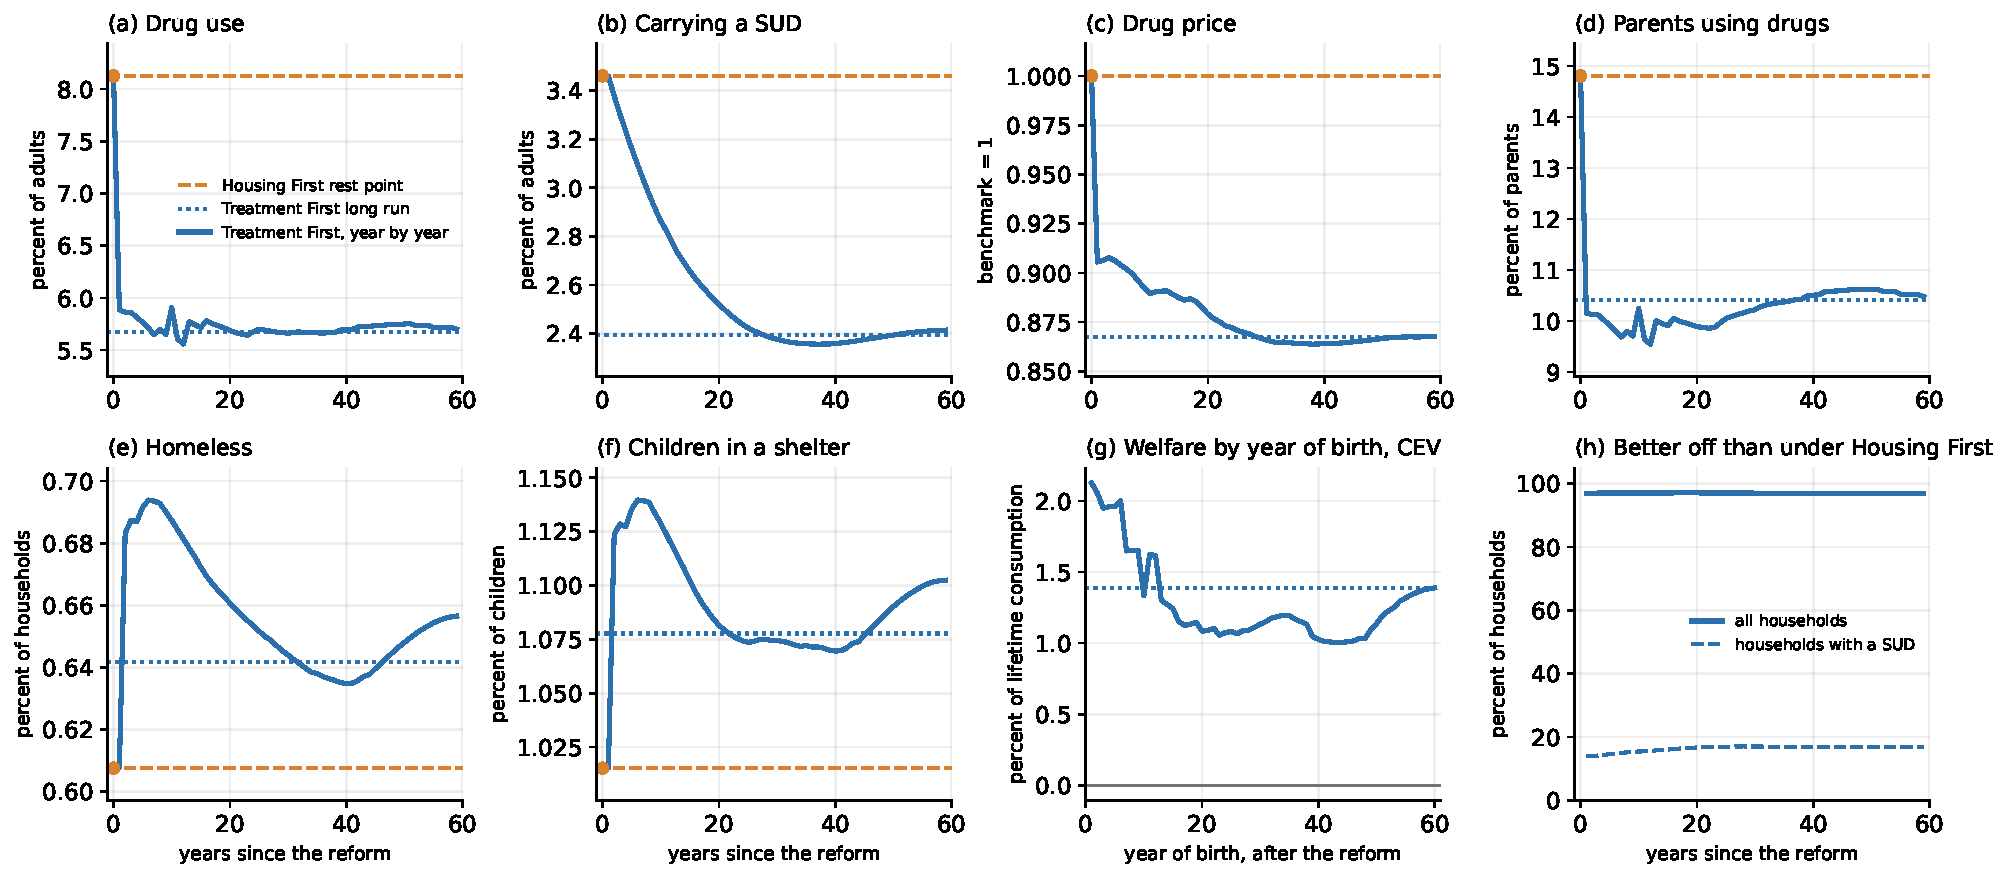
\includegraphics[width=\textwidth]{figures/full_transition.pdf}
\caption{The transition from Housing First to Treatment First, quantitative model}\label{fig:ftrans}
\notes{\textwidth}{Notes: panels (a) to (f) and (h) are by year since the reform, which lands at
the start of year 1, with the benchmark as year 0; the dashed orange line is the Housing
First benchmark, the dotted blue line the Treatment First long run and the solid blue line
the path. Children are those of households aged 26 to 50. Panel (g) is the CEV of each cohort
born on the path, against the benchmark, by its year of birth. Panel (h) is the share of households better off in each year of the path than in the
same state under Housing First, weighted by the benchmark's distribution.}
\end{figure}

Panels (a) and (d) show drug use and the share of parents who use, respectively. Drug use falls upon impact: $@@x_trf_b1_share_pc@@$ percent of its long-run fall happens in
the first year. The share of parents using drugs falls from $@@x_trf_paruse0@@$ to $@@x_trf_paruse1@@$ percent, @@x_trf_paruse1_vs_lr@@ its long-run level of $@@x_trf_paruse_lr@@$ percent. These shares drop because the screen acts on the decision to use from the day the reform lands, and households who do not have a SUD have agency over whether they use drugs or not: a
household that uses risks losing its voucher within a year, or having a voucher offer revoked later, when it may need one but have a SUD, while a disorder takes years to clear.

Panel (b) shows the
share with a SUD. This share falls slowly, because recovery is slow: half of its
long-run fall is done by year $@@x_trf_sud_half_yr@@$, and nine tenths by year
$@@x_trf_sud_90_yr@@$. That stock keeps demand for the drug up, and the drug price stays
above its long-run level for $@@x_trf_price_above_yrs@@$ years (panel (c)). The elevated price deters
households without a SUD, at every age: in the first decade the number of drug users without
a SUD falls by up to $@@x_tr_new_peak_pc@@$ percent, against $@@x_tf_new_pc@@$ percent in the
long run. The share of parents who use stays above its long-run level all the same, because it counts the parents who have a SUD, whose number falls only slowly (panel (b)). @@x_trf_paruse_why@@

Panels (e) and (f) show homelessness and the share of children in a shelter, respectively. Homelessness overshoots. It rises by $@@x_trf_h_peak_pc@@$ percent at its peak, in year $@@x_trf_h_peak_yr@@$, @@x_trf_h_tail@@. @@x_trf_h_why@@ A similar pattern is observed for childhood homelessness: the share of children in a
shelter rises from $@@x_trf_hchild0@@$ to
$@@x_trf_hchild_peak@@$ percent in year $@@x_trf_hchild_peak_yr@@$, against
$@@x_trf_hchild_lr@@$ percent in the long run. It rises for the same reason: the parents who have a SUD when the reform lands lose their vouchers within a year, and it comes back down only as their number falls.

Panel (g) shows the CEV of each cohort by its year of birth. Children born at the reform gain about $@@x_tr_cev_b1@@$ percent of lifetime
consumption, @@x_tr_cev_b1_vs_lr@@. They gain, because the fall in parental drug use reaches far more children than the overshoot in homelessness@@x_trf_many@@. They gain less than in the long run, because they grow up while the share of parents with a SUD is still close to its Housing First level, since that share falls only as fast as recovery allows, so more of them spend their childhood with a parent who has the disorder, and more enter adult life with the earnings penalty. The gain stays near that level for children born while that share is still falling, and rises toward the long run for those born later, whose parents were themselves born after the reform.

Of the adults alive at the reform, only $@@x_trf_alive_worse_pc@@$ percent are worse off under it, and even
$@@x_trf_alive_sud_better_pc@@$ percent of those who have a SUD when it lands benefit, because the lower drug
price more than offsets the loss from the sobriety requirement for some of them. @@x_trf_better_sentence@@ A newborn's comparison also counts its childhood, which may be spent with a parent who loses a voucher, so fewer newborns than entering adults gain: in the long run, $@@x_lr_nb_better_pc@@$ percent are better off than if born into the same household under Housing First (Table~\ref{tab:longrun}).

%======================================================================
\section{Discussion and implications}\label{sec:discussion}

To return to the question I started with: should housing assistance require sobriety? When households are forward looking and weigh the true risk of a
SUD, the moral hazard that dominates the debate over this question does not justify conditionality: without externalities, and at fixed prices and access to vouchers,
Housing First wins. What turns the ranking are externalities imposed on children. In the long run of a
general-equilibrium model calibrated to United States data, Treatment First cuts drug use by
$@@x_tf_b_pc@@$ percent and the share of households with a SUD by $@@x_tf_sud_pc@@$ percent, and actually @@x_tf_h_dir@@
homelessness by $@@x_tf_h_pc@@$ percent. As a result, it raises the welfare of a newborn by $@@x_tf_cev@@$ percent of lifetime
consumption. Most of that gain comes in childhood, from parents who spend less on drugs and are less likely to remain unemployed because of a SUD after losing their job. The
rest comes from better earnings and from a larger voucher programme, which the users it excludes and the higher revenues from the taxes paid by more productive and more employed
households pay for.

@@x_disc_tr_kids@@ Yet, from a policy point of view the transition can be deceptive. The households that have a SUD
when the reform lands lose their vouchers within a year, so
homelessness first rises, by up to $@@x_trf_h_peak_pc@@$ percent, and the share of children in a shelter with it. It
comes down only as the number with a SUD falls, which takes $@@x_trf_sud_90_yr@@$ years to complete nine tenths
of its fall. And of those with a SUD at the reform, only $@@x_trf_alive_sud_better_pc@@$ percent are better off.

Three lessons follow. First, the arguments for Housing First and Treatment First made by different advocacy
groups leave out the outcome that matters most: what happens to the children of the households a sobriety requirement deters from using, in what they consume while at home and in what they earn as adults. If this framing continues to dominate the discussion, the reform will most likely be judged on the wrong outcomes.

Second, the politics of the reform can run against its own payoff. Its apparent costs would come first, falling on
households already having a SUD, and would appear in the homelessness counts during the transition from the Housing
First benchmark to the long-run equilibrium under Treatment First; its positive effects on homelessness would only come
later. Judged even on its first 25 years, by the PiT count, the reform will look like a failure exactly
when the model's reading is that it is on course, and it will be most exposed to reversal before its long-run positive effects on
homelessness, the SUD and, most importantly, children have arrived in full.

Third, the results point to two choices of design that the current debate leaves out. The first is what to do
with the excess funds the government collects under Treatment First. In my
experiment, all of them go back into vouchers, so an eligible household that does not use drugs is
$@@x_tf_piv_pc@@$ percent more likely to get one, which is one of the reasons a newborn's adult life is worth
more@@x_disc_recycle_h@@. A sobriety requirement introduced without recycling that excess revenue back into more
vouchers would give up @@x_dc_pv_share_word@@ the gain: with $\pi_V$ held at its benchmark level, a newborn would gain
$@@x_dc_pv_cev@@$ percent rather than $@@x_tf_cev@@$, and homelessness would @@x_dc_pv_h_dir@@ by $@@x_dc_pv_h_pc@@$ percent.

The second is whom the condition applies to, which may further mitigate the impact on the households that
already have a SUD along the transition. The gain comes from deterrence: adults who do not have a SUD and are able to stay clean do so to keep their
access to a voucher. The early cost falls on a different group, the households that already have a SUD when the
reform lands. They cannot respond quickly, because recovery from a SUD is slow, so for them the condition brings
mostly the cost. Their homelessness rises within a year, and $@@x_trf_alive_sud_worse_pc@@$ percent of them are worse off. A condition applied only to new voucher holders, with current holders given a five-to-ten-year grandfather exemption, for example,
may strike a good balance between keeping the threat
for those who can still respond to it and sparing those who cannot.

\clearpage
\appendix
\setcounter{table}{0}\renewcommand{\thetable}{A\arabic{table}}
\section[Calibration of the standard parameters]{\new{Calibration of the standard parameters}}\label{sec:stdparams}

The remaining @@n_std@@ parameters are more conventional, and I record the
values I use so that the calibration can be reproduced. @@n_std_int_cap@@ of them I calibrate internally,
against a moment, because no source reads them off directly; the other @@n_std_ext@@ I set
from outside, from an estimate or from statute. Table~\ref{tab:stdparams} and the
entries below run in the same seven blocks, and each entry gives the moment or the
source that fixes the parameter together with the value that moment takes in the
data. The Model column reports what the model produces against that value, and it
does so only for the @@n_std_int@@ I calibrate internally, since the other
@@n_std_ext@@ have no target to reproduce.

The parameters in this appendix are not inert in the experiments. For example, the discount
factor governs how heavily a household weighs a death later in life, the dispersion
of productivity determines how many households are poor enough to be at risk of
homelessness and of acquiring a disorder, and risk aversion governs what insurance
is worth. What separates them from the parameters above is not that they do nothing,
but that they are not specific to this paper.

\begin{table}[htbp]\centering
\caption{Standard parameters}\label{tab:stdparams}
\begingroup\scriptsize\setlength{\tabcolsep}{3pt}
\begin{tabular}{@{}lL{3.6cm}cL{5.5cm}rrr@{}}
\toprule
Parameter & Description & Set & Moment and source & Data & Model & Value \\
\midrule
\multicolumn{7}{@{}l}{\textcolor{red}{\emph{Preferences}}} \\
$\sigma$ & Risk aversion & Ext. & Attanasio and Weber (2010) & 2.00 & n.a. & 2.00 \\
$\gamma$ & CD weight on housing & Int. & Renters above 30 pct of income, ACS 2023 & 49.7\% & \textemdash & \textemdash \\
$\beta$ & Discount factor & Int. & Wealth over output, BEA fixed assets & 3.00 & \textemdash & \textemdash \\
\textcolor{red}{$\omega_{\ell}$} & \textcolor{red}{Weight on leisure} & \textcolor{red}{Int.} & \textcolor{red}{Average hours worked, Guvenen et al.\ (2023)} & \textcolor{red}{0.40} & \textemdash & \textemdash \\
\addlinespace
\multicolumn{7}{@{}l}{\textcolor{red}{\emph{The rental ladder}}} \\
$\underline h$ & Smallest rental size & Int. & Share in smallest unit size, ACS 2023 & 13.2\% & \textemdash & \textemdash \\
$\bar h$ & Largest rental size & Int. & Share in largest unit size, ACS 2023 & 62.7\% & \textemdash & \textemdash \\
$\varsigma$ & Curvature of the ladder & Ext. & Set; the two ends carry the distribution & 1.80 & n.a. & 1.80 \\
\addlinespace
\multicolumn{7}{@{}l}{\textcolor{red}{\emph{Earnings and employment}}} \\
$\varepsilon(j)$ & Age profile of efficiency & Ext. & Quadratic in age, PSID and CPS hump & profile & n.a. & profile \\
$\rho_y$ & Persistence of log prod. & Ext. & Storesletten et al.\ (2004) & 0.90 & n.a. & 0.90 \\
$\sigma_y$ & Dispersion of log prod. & Ext. & Storesletten et al.\ (2004) & 0.20 & n.a. & 0.20 \\
$\bar\pi^{eu}$ & Job separation rate & Int. & Unemployment rate, BLS CPS 2014--24 & 4.85\% & \textemdash & \textemdash \\
$\bar\pi^{ue}$ & Job finding rate, annual & Ext. & Krueger, Cramer and Cho (2014) & 0.55 & n.a. & 0.55 \\
\addlinespace
\multicolumn{7}{@{}l}{\textcolor{red}{\emph{Survival and mental illness}}} \\
$\bar\phi(j)$ & Baseline survival by age & Ext. & SSA period life table, ages 26 to 85 & profile & n.a. & profile \\
$p_m$ & Age profile of SMI prevalence & Ext. & Share with SMI, NSDUH 2023 & 5.5\% & n.a. & 5.5\% \\
\addlinespace
\multicolumn{7}{@{}l}{\textcolor{red}{\emph{Interest, taxes and public spending}}} \\
$r$ & Risk free rate & Ext. & Kaplan, Mitman and Violante (2020) & 0.03 & n.a. & 0.03 \\
$\xi$ & Tax progressivity & Ext. & Heathcote et al. (2017) & 0.85 & n.a. & 0.85 \\
$\tau_k$ & Capital income tax & Ext. & US long run rate on gains and dividends & 0.15 & n.a. & 0.15 \\
$\tau_{\ell}$ & Tax level & Ext. & Clears the government budget & in eqm. & n.a. & in eqm. \\
$G$ & Other public spending & Ext. & Residual at benchmark, then held fixed & in eqm. & n.a. & in eqm. \\
\addlinespace
\multicolumn{7}{@{}l}{\textcolor{red}{\emph{Transfers and the voucher rule}}} \\
$\psi$ & UI replacement rate & Ext. & DOL statutory replacement rates & 0.50 & n.a. & 0.50 \\
$\bar y$ & Cap on insurance earnings & Ext. & DOL state benefit maxima & 1.00 & n.a. & 1.00 \\
$\kappa_V$ & Voucher eligibility cutoff & Ext. & HUD rule & 0.50 & n.a. & 0.50 \\
$\kappa_r$ & Tenant contribution rate & Ext. & HUD rule & 0.30 & n.a. & 0.30 \\
\addlinespace
\multicolumn{7}{@{}l}{\textcolor{red}{\emph{The drug market}}} \\
$j_E$ & Last experimentation age & Ext. & Reported with and without it & 55 & n.a. & 55 \\
\textcolor{red}{$\nu_1$} & \textcolor{red}{Drug supply shifter} & \textcolor{red}{Ext.} & \textcolor{red}{Normalisation, so $p_v=1$} & \textcolor{red}{norm.} & \textcolor{red}{n.a.} & \textcolor{red}{norm.} \\
\textcolor{red}{$p_v$} & \textcolor{red}{Price of drugs} & \textcolor{red}{Ext.} & \textcolor{red}{Clears the drug market in the benchmark} & \textcolor{red}{1.00} & \textcolor{red}{n.a.} & \textcolor{red}{1.00} \\
\bottomrule
\end{tabular}
\notes{\textwidth}{Note: n.a.\ in the Model column marks a parameter that is set from outside rather than calibrated inside the model. For those the model produces no internal target to compare with the data, so the cell reads n.a.\ rather than a dash, which keeps them distinct from the internally calibrated parameters.}
\endgroup
\end{table}



\paragraph{Block 7: Preferences.} The four parameters in this block determine what a household wants, and what it is willing to give up to get it.
\begin{description}\setlength{\itemsep}{0.25em}\setlength{\parskip}{0em}
\item[$\sigma$, risk aversion.] It sets the marginal utility of consumption, so it
affects every welfare comparison in the paper. Increase it and households want smoother
consumption and insurance is
worth more, which then means that the voucher is worth more. I set it to the standard value of two, following
Attanasio and Weber (2010).
\item[$\gamma$, the weight on housing services.] It is the weight on housing in the
bundle of consumption and housing, so it sets what a dwelling is worth against
consumption, and that bundle is what the drug is weighed against. As
$\gamma$ rises housing is worth more relative to consumption, households buy more of it,
and the share of spending that goes on housing rises with it. $\gamma$ is chosen for the share
it produces: shelter plus utilities take $@@c_gamma_data@@$ percent of expenditure in the 2024 CEX, which excludes illicit drug spending.
\item[$\beta$, the discount factor.] It sets how much households discount the
future, and thus how much they save and how much the prospect of death deters them from using drugs. As it rises households save more, the
 wealth-to-output ratio rises and households are more deterred by death. It is chosen so that wealth over output
matches the national accounts, a ratio of three, from the Bureau of Economic Analysis (BEA) fixed asset tables
against National Income and Product Accounts (NIPA) output, both read at the 2023 vintage, the last year the fixed asset tables cover.
\item[$\xi_j$, the equivalence scale.] The household's consumption and
dwelling are shared with the child while it lives with its parent, and thus are divided by
$\xi_j$ to give what each member gets. Raise it and each member gets less of a given budget, and the child counts for more of the household, through the weight $\xi_j-1$ in~\eqref{eq:futil}. It is the square-root scale, $\sqrt{N_j}$, where $N_j$ in the model is set to two while
the child lives with the parent ($j\le J_K$), from the parent's age 26 to 50, and to one after the child has left ($j>J_K$).
\end{description}

\paragraph{Block 8: Rental ladder.} These three parameters build the grid of dwelling
sizes a household chooses from. Below the smallest rung is the shelter, $h_1$, which was calibrated in Block 2.
\begin{description}\setlength{\itemsep}{0.25em}\setlength{\parskip}{0em}
\item[$h_2$, the smallest rental size.] The size of the cheapest dwelling is what
decides how much of its income a poor household must spend to be housed at all. Raise it and the bottom rung is
larger and dearer, so more households are burdened, and a voucher is worth more to them. It is chosen so that
the fraction of renters paying more than half of their income for housing is similar to
the data, $@@c_h_2_data@@$ percent in the 2022 SCF; the model gives $@@c_h_2_model@@$
percent.
\item[$h_3/h_2$ and $h_4/h_2$, the spacing of the ladder.]  The second and upper rungs set how much housing  they provide, and so what a household that can afford more than the smallest unit can move up to. Raise them and each step up the ladder costs more rent, and fewer households can rent them. The two larger
rungs are set at $@@c_h_3_h_2_value@@$ and $@@c_h_4_h_2_value@@$ times the smallest.
\end{description}

\paragraph{Block 9: Earnings and employment.} These ten parameters determine how long a household
lives and works, what it
is expected to earn over its life, how persistent the shocks to it are, and how it
moves between work and unemployment.
\begin{description}\setlength{\itemsep}{0.25em}\setlength{\parskip}{0em}
\item[$J$, $J_K$ and $J_R$, the length of life, of child rearing and of working life, respectively.] A household lives at most
$J$ periods, has its child at home for its first $J_K$ of them and works until age $J_R$, after which it retires on social security.
Together they set how many years of life and of earnings a disorder can cost, and $J_K$ how long a parent's drug use reaches their child through what they share. Raise
either $J$ or $J_R$ and a disorder that shortens life or work costs more; raise $J_K$ and the budget  and childhood homelessness externalities last longer. I set $J=@@c_j_value@@$, so
that with $j=1$ at age 26 the last age is $@@c_j_age@@$, $J_K=@@c_j_k_value@@$, so that the child lives at home while its parent is 26 to $@@c_j_k_age@@$, and $J_R=@@c_j_r_value@@$, so that retirement begins at age $@@c_j_r_age@@$, the
full retirement age under social security for those born between 1943 and 1954.
\item[$\varepsilon(j)$, the age profile of efficiency.] This is the deterministic hump in
earnings over the life cycle. Without it every
household with the same productivity would earn the same at every age, and the ages at which households are
poor, and so at risk of homelessness and of using, would be wrong at both ends of
working life. I take it as the exponential of a quadratic in age used by
Greenwood et al.\ (2025), $\varepsilon(j)=\exp\{-(j-1)^2/1800+(j-1)/30\}$ with $j=1$
at age $26$. It peaks at age $56$, having risen $65$ percent from age $26$, and then
falls $4$ percent from the peak to age $65$, the last working age.

\item[$\rho_z$ and $\sigma_\zeta$, the productivity process.] Log
productivity is persistent but not permanent: it follows an autoregressive process
with persistence $\rho_z$ and shocks with standard deviation
$\sigma_\zeta$. $\sigma_\zeta$ is what decides how many households are poor
enough to be at risk of homelessness, and the share of earnings
that goes to the bottom half of working households falls in it. I set
$\rho_z=@@c_rho_z_value@@$, the persistence of the income process in Guvenen et al.\ (2023). $\sigma_\zeta$
is calibrated to the bottom half's share of earnings among households aged 26 to 65 with
positive wage income in the 2022 SCF, $@@c_sigma_zeta_data@@$ percent.

\item[$\rho$, the persistence of productivity across generations.] The
child's log productivity at entry into adulthood is drawn around its parent's with weight $\rho$ and
around the mean with weight $1-\rho$, so $\rho$ is how much of its parent's current productivity a
child keeps. It is the channel through which anything that lowers a parent's productivity lowers their child's: a parent whose own productivity carries the penalty $\delta_d$, because their own parent had a SUD, also passes a lower draw on to their child, so a
parent's SUD lowers productivity beyond the next generation. Raise it and a child's prospects depend more
on its parent's decisions, and the earnings externality grows. It is set
externally at $@@c_rho_value@@$, between the intergenerational elasticities of earnings
in Solon (1992) and Mazumder (2005).
\item[$\bar\pi^{eu}$, the job separation rate.] This parameter determines the chance that an employed household
loses its job each year. It is scaled by $\varpi(y)$ in~\eqref{eq:femp}, so separations are likelier at low
productivity. Raise it and more households lose work each year, so the unemployment
rate rises with it. It is chosen to reproduce the aggregate
unemployment rate in the BLS CPS over 2014 to 2024,
$@@c_bar_pi_eu_data@@$ percent, given the job-finding rate set externally below.
\item[$\varpi(y)$, separations by productivity.] This parameter tilts the separation rate across
productivity, so that low-productivity households lose their jobs more often, which is what
puts them at a higher risk of homelessness. Steepen the tilt and job loss concentrates further among the poorest, and so does the risk of homelessness. It is normalised to average one across households, so
that $\bar\pi^{eu}$ alone sets the aggregate unemployment rate. Each productivity node takes the
unemployment odds of the education group it falls in, from the BLS 2019 annual averages of
unemployment by educational attainment for ages 25 and over, with education ordering
productivity by median earnings.
\item[$\bar\pi^{ue}$, the annual job-finding rate.]  This parameter is the probability that an
unemployed household finds work each year it is unemployed. With the divisors $\kappa^{ue}_{d}$ and $\kappa^{ue}_{m}$ it sets how long an unemployed household with a SUD or SMI is expected to remain unemployed. Raise it and spells out of work are shorter on average, so fewer households fall behind on the rent. I set it to
$@@c_bar_pi_ue_value@@$ from the annual exit rate Krueger et al.\ (2014) estimate on
matched CPS panels.
\item[$p_{ui}$, the share of separations that receive UI.] A household that
loses its job draws UI for one year with probability $p_{ui}$ and nothing
otherwise. It sets how many of the newly unemployed fall straight to zero
earnings, and how costly being unemployed is. I set it to $@@c_p_ui_value@@$, since about seven in ten unemployed people who
worked in the past year did not apply for UI after losing their job in the BLS
supplement to the CPS for 2022.
\end{description}

\paragraph{Block 10: Baseline survival and SMI onset.} These two parameters are the survival and
the SMI-onset age profiles.
\begin{description}\setlength{\itemsep}{0.25em}\setlength{\parskip}{0em}
\item[$\bar\phi_j$, baseline survival by age.] This is the baseline chance of surviving to the
next age, before any multiplier. It is the profile every mortality multiplier in
Section~\ref{sec:fullcal} multiplies, so it is the base the SUD, homelessness and
SMI hazards scale. Raise it and households expect to live longer, so the life a SUD puts at risk is worth more. I take the profile from  the life table for the total population of the United States in 2010 (Arias, 2014), for ages $26$ to $85$.

\item[$\varsigma_m(j)$, the age profile of SMI onset.] This determines the shape of onset
across ages, normalised to one at age $26$, so that $\omega_m$ in Table~\ref{tab:eleven} sets its
level alone. It is here rather than in Table~\ref{tab:eleven} because, like the age survival profile, it only sets the
baseline; what actually affects the impact of Housing First versus Treatment First is $\iota$, the multiplier a SUD puts
on SMI onset, which is in Table~\ref{tab:eleven}. It is the onset that
reproduces a log-linear fit to the share of adults carrying SMI at each age in NSDUH
2024.
\end{description}

\paragraph{Block 11: Interest and taxes.}
\begin{description}\setlength{\itemsep}{0.25em}\setlength{\parskip}{0em}
\item[$r$, the risk-free rate.] This parameter sets the return on saving. Raise it and saving pays more, so households hold more assets to carry them through a spell out of work or without a voucher. I set it to three percent, from Kaplan et al.\
(2020).

\item[$\varphi$, tax progressivity.] This is the exponent on income in the tax schedule of
Section~\ref{sec:ftaxes}, and it determines the progressivity of the labour income tax. Lower it and the tax is more progressive, so households with low incomes, among them most voucher holders and most drug users, keep more of what they earn. It is set to $@@c_varphi_value@@$, in line with Heathcote et al.\ (2017). 

\item[$\tau_{\ell}$, the scale of after-tax labour income.] Given $\varphi$, this parameter sets how much
of their labour income households keep after tax on average, so raising it lowers the tax liability. It does not move in the experiments: the budget is
balanced by $\pi_V$ instead. It is calibrated  to
an average labour income tax rate of $@@c_tau_ell_data@@$ percent,
which is what McDaniel (2007) measures for the United States and what Guvenen et al.\ (2023) use.

\item[$\tau_k$, the capital income tax rate.] This parameter affects the after-tax return on savings. Raise it and saving pays less, so households hold fewer assets to fall back on. I set it to fifteen percent, consistent
with the statutory United States rate on long-term capital gains and qualified
dividends for the middle of the income distribution, which the Internal Revenue
Service (IRS) sets out in Topic 409
(\url{https://www.irs.gov/taxtopics/tc409}).

\end{description}

\paragraph{Block 12: Social security benefits and programmes' rules.}
\begin{description}\setlength{\itemsep}{0.25em}\setlength{\parskip}{0em}
\item[$S(y)$ and $\underline S$, social security and its floor.] Retirement income follows the statutory
primary insurance amount: it replaces a share of the household's income at its last working
age that falls across the two bend points of the Social Security Administration (SSA), up to
the taxable maximum, and with the SSI payment as a floor (the full function is detailed in footnote~\ref{fn:ss}). As $S(y)$ rises the old are richer, so the value of a life
still to be lived rises and with it the cost of a disorder that shortens it. The shares
$\alpha_1,\alpha_2,\alpha_3$ are $@@c_s_y_value@@$ below the first bend point, between them and above the second, respectively. The
bend points $k_1$ and $k_2$ and the taxable maximum $y^{\max}$ are the SSA's 2024 dollar
amounts divided by its average wage index, $@@f_ss_bend_1@@$, $@@f_ss_bend_2@@$ and
$@@f_ss_taxable_max@@$, respectively. The floor, $\underline S$, is $@@c_underline_s_value@@$ of average
labour income.
\item[$\psi_{ui}$ and $\bar y$, UI.] These two set the UI replacement
rate and the cap on the earnings it is paid on, respectively. Raise either and the first year out of work costs a household less, so a spell out of work is less likely to end in a shelter. I set them to fifty percent and one
times average labour income, respectively, taking both from the statutory replacement rates
and state benefit maxima that the Department of Labor compiles in its comparison of
state UI laws
(\url{https://oui.doleta.gov/unemploy/statelaws.asp}).

\item[$\kappa_V$ and $\kappa_r$, the voucher rules.] These two set the income
cutoff for eligibility and the tenant's rent contribution, respectively. Raise $\kappa_V$ and more households are eligible, so more have a voucher to lose under Treatment First; raise $\kappa_r$ and a voucher pays less, so there is less to lose from losing a voucher. I take both from HUD's own
rules. I set them to half of median income and thirty
percent, respectively. The first is the very low-income limit HUD publishes
annually with its income limits
(\url{https://www.huduser.gov/portal/datasets/il.html}); the second is the share of its before-tax income a tenant pays towards the rent, the voucher
paying the rest up to the payment standard, under the Housing Choice
Voucher programme
(\url{https://www.hud.gov/helping-americans/housing-choice-vouchers}).

\item[$\varrho$, the food stamp clawback rate.] This is the rate at which food assistance is withdrawn as income rises. Raise it and food assistance is clawed back faster, so it stops at a lower income and pays less to every household that still receives it. I set it to thirty percent, which is the statutory rule (7 CFR 273.10).
\end{description}

\paragraph{Block 13: Drug market.} The two parameters in this block describe the rest of the drug
market, closing the loop on the elasticity explained in Block 6: the first fixes who can
enter it, and the second is set so that supply equals demand in the benchmark, and is
then held fixed.
\begin{description}\setlength{\itemsep}{0.25em}\setlength{\parskip}{0em}
% THE PARENTHETICAL BELONGS IN THE BODY, NOT THE LABEL. A description
% label does not wrap: it is typeset on one line and runs off the page,
% which is what it did here.

\item[$J_E$, the maximum age at which use can begin.] This restricts only households that do not have a SUD, not ones that already do.
It is there so that use cannot begin in the last few years of life, where almost no
continuation value remains to be lost. That is an artefact of the horizon rather than a feature of the world:
the model imposes certain mortality after age $85$,
so a household near the end knows death is coming with certainty and a disorder costs
it almost nothing. Without the cap the model would let use begin exactly there, and
at the final age it would be worse than that, since a household that acquires the
disorder in the last period dies at the end of it whatever the hazard does: the
disorder carries literally no consequence and the household can only stand to benefit from
the drugs. I set it to fifty-five in model terms, which corresponds to age $80$ in the data, very close to the maximum age of $@@c_j_age@@$.

\item[$\nu_1$, the supply shifter.] A pure normalisation, chosen so that supply
equals demand at $p_v=1$ in the benchmark, and kept fixed across experiments, in which
the price is free. It normalises units, not behaviour.

\end{description}

\clearpage


\section[Full altruism and full internalisation]{\new{Full altruism and full internalisation}}\label{sec:altruism}

\new{This appendix reports two benchmarks that set the scale of the externalities rather than compare the two policies: full altruism, in which a parent weighs their child as themselves, $\omega_c=1$, so that nothing a parent does to their child is left external; and full internalisation, which adds each household weighing the disamenity its own homelessness imposes on everyone else. Neither has a CEV, because each changes the welfare function itself.}

\new{In the stylized model, I set the weight a parent puts on their child to one,
$\omega_c=1$, so that a parent counts their child fully, with nothing else changed and the
programme left as it is. In this case, no parent uses at all: participation and the SUD rate
both fall to $@@s4_part_opt@@$ percent, and homelessness to $@@s4_homeless_opt@@$ percent.}

\new{The second column of Table~\ref{tab:altruism} keeps Housing First but has each parent weigh their child as themselves,
$\omega_c=1$: the drug use parents would choose if they took in full what their use does to
their children. A parent who counts their child's consumption as their own uses less of the
drug, and some parents stop altogether. What it spends on the drug (and any earnings it loses while it remains unemployed longer because of a SUD) comes out of the bundle
it shares with the child, and a SUD penalises the child's earnings. But, because supply is not perfectly elastic, the fall in demand then lowers the drug price, which draws some of them
back.

Notice that @@x_lr_tf_vs_om2@@. Under full altruism homelessness @@x_lr_om_h_dir@@ by $@@x_lr_om_h_pc@@$
percent, and the share of children in a shelter @@x_lr_om_hchild_dir@@ by
$@@x_lr_om_hchild_pc@@$ percent. @@x_lr_om_h_why@@ Treatment First, by contrast, @@x_lr_tf_both@@.

@@x_lr_om_piv_sentence@@ @@x_lr_om_piv_why@@

The third column is the same as full altruism, with the
addition of each household weighing the disamenity its own homelessness imposes on everyone else.
It @@x_lr_in_dh_verb@@ homelessness by only $@@x_lr_in_dh_pc@@$ percent on top of what @@x_lr_in_base_word@@ achieves,
because the externality turns out to be very small. Households can save and use less of the drug
to improve their housing outcomes@@x_lr_in_many_do@@. Nevertheless, the disamenity their homelessness imposes on others
is not a strong enough deterrent, so weighing it does not alter their behaviour significantly.
@@x_lr_in_piv_sentence@@}

\begin{table}[!tb]\centering
\caption{\new{Full altruism and full internalisation in the long run}}\label{tab:altruism}
\begingroup\scriptsize
\sbox{\ntbox}{% Written by code/paper/export_longrun.py from results/counterfactuals_cf_fix2;
% edit the script, not this file. Caption and note are in the paper.
\begin{tabular}{@{}lrrr@{}}
\toprule
 & Housing & Full & Full \\
 & First & altruism & internalisation \\
\midrule
\multicolumn{4}{@{}l}{\emph{Adults}} \\
Drug price, benchmark $=1$ & 1.00 & 0.88 & 0.88 \\
Voucher probability $\pi_V$ & 6.75 & 5.84 & 5.85 \\
Drug use & 8.96 & 7.45 & 7.44 \\
Carrying a SUD & 3.81 & 3.13 & 3.13 \\
Homelessness & 0.62 & 0.56 & 0.55 \\
SUD share of the homeless & 20.2 & 13.3 & 13.3 \\
In treatment, of those with a SUD & 24.9 & 25.2 & 25.2 \\
\addlinespace
\multicolumn{4}{@{}l}{\emph{Children}} \\
Living with a parent who uses drugs & 16.32 & 13.48 & 13.47 \\
Living with a parent who has a SUD & 5.81 & 4.78 & 4.78 \\
In a shelter & 1.03 & 0.89 & 0.87 \\
\addlinespace
\multicolumn{4}{@{}l}{\emph{Welfare}} \\
CEV of a newborn, percent of lifetime consumption & -- & -- & -- \\
Share of the newborn's gain that comes in childhood & -- & -- & -- \\
Households entering adult life at 26 better off & -- & -- & -- \\
All households better off & -- & -- & -- \\
Households with a SUD better off & -- & -- & -- \\
Newborns better off, by the household they are born into & -- & -- & -- \\
\bottomrule
\end{tabular}
}\usebox{\ntbox}
\tabnote{\new{Notes: long-run steady states, percent unless the row says otherwise. Housing First is the benchmark. Full altruism is Housing First with $\omega_c=1$, and full internalisation adds to it each household weighing the disamenity of its own homelessness; in both, the drug price clears and $\pi_V$ holds net government revenue at its benchmark level. Children are those living with households aged 26 to 50.}}
\endgroup
\end{table}
\clearpage


\section*{References}



{\normalsize
\setlength{\parindent}{0em}
\begin{list}{}{\setlength{\leftmargin}{1.5em}\setlength{\itemindent}{-1.5em}\setlength{\itemsep}{0.35em}\setlength{\parsep}{0em}}
\item Abramson, B. (2026). ``The Equilibrium Effects of Eviction Policies.'' \emph{Journal of Finance}, published online, \url{https://doi.org/10.1111/jofi.70046}.
\item AFCARS. \emph{Adoption and Foster Care Analysis and Reporting System}, US Department of Health and Human Services, Administration for Children and Families, FY2017 and FY2025 releases.
\item Altonji, J., F. Hayashi and L. Kotlikoff (1997). ``Parental Altruism and Inter Vivos Transfers: Theory and Evidence.'' \emph{Journal of Political Economy} 105(6), 1121--66.
\item Arias, E. (2014). ``United States Life Tables, 2010.'' \emph{National Vital Statistics Reports} 63(7). Hyattsville, MD: National Center for Health Statistics.
\item {\AA}sb{\o}, G. et al.\ (2022). ``The Time Is Ripe for a Consensus Definition of Clinical Recovery in First-Episode Psychosis: Suggestions Based on a 10-Year Follow-Up Study.'' \emph{Schizophrenia Bulletin} 48(4), 839--49.
\item Attanasio, O. P. and G. Weber (2010). ``Consumption and Saving: Models of Intertemporal Allocation and Their Implications for Public Policy.'' \emph{Journal of Economic Literature} 48(3), 693--751.
\item Aubry, T. et al.\ (2016). ``A Multiple-City RCT of Housing First With Assertive Community Treatment for Homeless Canadians With Serious Mental Illness.'' \emph{Psychiatric Services} 67(3), 275--81.
\item Bassuk, E. L., J. C. Buckner, L. F. Weinreb, A. Browne, S. S. Bassuk, R. Dawson and J. N. Perloff (1997). ``Homelessness in Female-Headed Families: Childhood and Adult Risk and Protective Factors.'' \emph{American Journal of Public Health} 87(2), 241--248.
\item Becker, G. S. and K. M. Murphy (1988). ``A Theory of Rational Addiction.'' \emph{Journal of Political Economy} 96(4), 675--700.
\item Bradizza, C. M., P. R. Stasiewicz and N. D. Paas (2006). ``Relapse to alcohol and drug use among individuals diagnosed with co-occurring mental health and substance use disorders: A review.'' \emph{Clinical Psychology Review} 26(2), 162--78.
\item Burt, M. R., L. Y. Aron and E. Lee (2001). \emph{Helping America's Homeless: Emergency Shelter or Affordable Housing?} Washington, DC: Urban Institute Press.
\item Card, D. (1999). ``The Causal Effect of Education on Earnings.'' In O. Ashenfelter and D. Card (eds.), \emph{Handbook of Labor Economics}, vol.\ 3A, 1801--63. Amsterdam: Elsevier.
\item Caulkins, J. P. (2001). ``Drug Prices and Emergency Department Mentions for Cocaine and Heroin.'' \emph{American Journal of Public Health} 91(9), 1446--48.
\item Chetty, R., N. Hendren, P. Kline and E. Saez (2014). ``Where is the Land of Opportunity? The Geography of Intergenerational Mobility in the United States.'' \emph{Quarterly Journal of Economics} 129(4), 1553--1623.
\item Chetty, R., N. Hendren and L. Katz (2016). ``The Effects of Exposure to Better Neighborhoods on Children.'' \emph{American Economic Review} 106(4), 855--902.
\item Chyn, E. (2018). ``Moved to Opportunity: The Long-Run Effects of Public Housing Demolition on Children.'' \emph{American Economic Review} 108(10), 3028--56.
\item Conesa, J. C., S. Kitao and D. Krueger (2009). ``Taxing Capital? Not a Bad Idea after All!'' \emph{American Economic Review} 99(1), 25--48.
\item \new{Costa, D.\ L.\ and M.\ E.\ Kahn (2004). ``Changes in the Value of Life, 1940--1980.'' \emph{Journal of Risk and Uncertainty} 29(2), 159--80.}
\item Costantini, S. (2025). ``Housing First or Treatment First? Evidence from the VA's Homelessness Programs.'' Working paper, University of California, Berkeley.
\item Dahl, G. B. and L. Lochner (2012). ``The Impact of Family Income on Child Achievement: Evidence from the Earned Income Tax Credit.'' \emph{American Economic Review} 102(5), 1927--56.
\item Degenhardt, L. et al.\ (2011). ``Mortality among regular or dependent users of heroin and other opioids: a systematic review.'' \emph{Addiction} 106(1), 32--51.
\item Desmond, M. and C. Gershenson (2016). ``Housing and Employment Insecurity among the Working Poor.'' \emph{Social Problems} 63(1), 46--67.
\item Felitti, V. et al.\ (1998). ``Relationship of Childhood Abuse and Household Dysfunction to Many of the Leading Causes of Death in Adults.'' \emph{American Journal of Preventive Medicine} 14(4), 245--58.
\item Fudala, P. J. et al.\ (2003). ``Office-based treatment of opiate addiction with a sublingual-tablet formulation of buprenorphine and naloxone.'' \emph{New England Journal of Medicine} 349(10), 949--958.
\item Gallet, C. A. (2014). ``Can Price Get the Monkey Off Our Back? A Meta-Analysis of Illicit Drug Demand.'' \emph{Health Economics} 23(1), 55--68.
\item Goering, P. et al.\ (2014). \emph{National At Home/Chez Soi Final Report}. Mental Health Commission of Canada.
\item Greenwood, J., N. Guner and K. A. Kopecky (2025). ``The Downward Spiral: A Macroeconomic Analysis of the Opioid Crisis.'' Working paper.
\item Grossman, M. and F. Chaloupka (1998). ``The demand for cocaine by young adults: a rational addiction approach.'' \emph{Journal of Health Economics} 17(4), 427--74.
\item Gruber, J. and B. K\H{o}szegi (2001). ``Is Addiction `Rational'? Theory and Evidence.'' \emph{Quarterly Journal of Economics} 116(4), 1261--1303.
\item Gutwinski, S., S. Schreiter, K. Deutscher and S. Fazel (2021). ``The prevalence of mental disorders among homeless people in high-income countries: An updated systematic review and meta-regression analysis.'' \emph{PLOS Medicine} 18(8), e1003750.
\item Guvenen, F., G. Kambourov, B. Kuruscu, S. Ocampo and D. Chen (2023). ``Use It or Lose It: Efficiency and Redistributional Effects of Wealth Taxation.'' \emph{Quarterly Journal of Economics} 138(2), 835--894.
\item \new{Hall, R.\ E.\ and C.\ I.\ Jones (2007). ``The Value of Life and the Rise in Health Spending.'' \emph{Quarterly Journal of Economics} 122(1), 39--72.}
\item Heathcote, J., K. Storesletten and G. Violante (2017). ``Optimal Tax Progressivity: An Analytical Framework.'' \emph{Quarterly Journal of Economics} 132(4), 1693--1754.
\item Heiberg, I. H. et al.\ (2018). ``Total and cause-specific standardized mortality ratios in patients with schizophrenia and/or substance use disorder.'' \emph{PLoS ONE} 13(8), e0202028.
\item Hjorth\o j, C., N. Albert and M. Nordentoft (2018). ``Association of substance use disorders with conversion from schizotypal disorder to schizophrenia.'' \emph{JAMA Psychiatry} 75(7), 733--739.
\item Hjorth\o j, C. et al.\ (2023). ``Excess mortality among people with substance use disorders.'' \emph{World Psychiatry} 22(2).
\item \.{I}mrohoro\u{g}lu, A. and K. Zhao (2022). ``Homelessness.'' Working paper.
\item Kaplan, G., K. Mitman and G. L. Violante (2020). ``The Housing Boom and Bust: Model Meets Evidence.'' \emph{Journal of Political Economy} 128(9), 3285--3345.
\item Krueger, A. B., J. Cramer and D. Cho (2014). ``Are the Long-Term Unemployed on the Margins of the Labor Market?'' \emph{Brookings Papers on Economic Activity}, Spring, 229--99.
\item Laibson, D. (1997). ``Golden Eggs and Hyperbolic Discounting.'' \emph{Quarterly Journal of Economics} 112(2), 443--77.
\item Larimer, M. E. et al.\ (2009). ``Health Care and Public Service Use and Costs Before and After Provision of Housing for Chronically Homeless Persons With Severe Alcohol Problems.'' \emph{JAMA} 301(13), 1349--57.
\item Larney, S. et al.\ (2020). ``All-cause and cause-specific mortality among people using extramedical opioids: a systematic review and meta-analysis.'' \emph{JAMA Psychiatry} 77(5), 493--502.
\item Legislative Budget Board (2013). ``Fiscal Note, 83rd Legislative Regular Session: SB 11.'' Texas Legislature, Austin.
\item Loubi\`ere, S. et al.\ (2020). ``Europeans' willingness to pay for ending homelessness: A contingent valuation study.'' \emph{Social Science \& Medicine} 247, 112802.
\item Lundborg, P. and B. Lindgren (2002). ``Risk Perceptions and Alcohol Consumption among Young People.'' \emph{Journal of Risk and Uncertainty} 25(2), 165--83.
\item Mace, C., E. Patel and N. Seegert (2020). ``Marijuana Taxation and Imperfect Competition.'' \emph{National Tax Journal} 73(2), 545--92.
\item Manchikanti, L., Y. Malla, B. W. Wargo and B. Fellows (2011). ``Comparative Evaluation of the Accuracy of Immunoassay with Liquid Chromatography Tandem Mass Spectrometry of Urine Drug Testing Opioids and Illicit Drugs in Chronic Pain Patients.'' \emph{Pain Physician} 14(2), 175--187.
\item Mazumder, B. (2005). ``Fortunate Sons: New Estimates of Intergenerational Mobility in the United States Using Social Security Earnings Data.'' \emph{Review of Economics and Statistics} 87(2), 235--255.
\item McDaniel, C. (2007). ``Average Tax Rates on Consumption, Investment, Labor and Capital in the OECD 1950--2003.'' Working paper, Arizona State University.
\item Mehay, S.\ L.\ and R.\ L.\ Pacula (1999). ``The Effectiveness of Workplace Drug Prevention Policies: Does `Zero Tolerance' Work?'' NBER Working Paper 7383.
\item Mellentin, A.\ I.\ et al.\ (2016). ``The risk of offspring developing substance use disorders when exposed to one versus two parent(s) with alcohol use disorder: a nationwide, register-based cohort study.'' \emph{Journal of Psychiatric Research} 80.
\item Meyer, B. D., A. Wyse, G. Meyer, A. Grunwaldt and D. Wu (2024). ``Homelessness and the Persistence of Deprivation: Income, Employment, and Safety Net Participation.'' NBER Working Paper 32323.
\item Meyer, B. D., A. Wyse and I. Logani (2023). ``Life and Death at the Margins of Society: The Mortality of the U.S. Homeless Population.'' NBER Working Paper 31843.
\item Midgette, G., S. Davenport, J. P. Caulkins and B. Kilmer (2019). ``What America's Users Spend on Illegal Drugs, 2006--2016.'' Santa Monica, CA: RAND Corporation.
\item Milby, J., J. Schumacher, D. Wallace, M. Freedman and R. Vuchinich (2005). ``To house or not to house: the effects of providing housing to homeless substance abusers in treatment.'' \emph{American Journal of Public Health} 95(7), 1259--65.
\item Murrie, B., J. Lappin, M. Large and G. Sara (2020). ``Transition of Substance-Induced, Brief, and Atypical Psychoses to Schizophrenia: A Systematic Review and Meta-analysis.'' \emph{Schizophrenia Bulletin} 46(3), 505--516.
\item Nielsen, S. M., N. B. Toftdahl, M. Nordentoft and C. Hjorthoj (2017). ``Association between alcohol, cannabis, and other illicit substance abuse and risk of developing schizophrenia: a nationwide population based register study.'' \emph{Psychological Medicine} 47(9), 1668--1677.
\item Nilsson, J. P. (2017). ``Alcohol Availability, Prenatal Conditions, and Long-Term Economic Outcomes.'' \emph{Journal of Political Economy} 125(4), 1149--1207.
\item OECD (2013). \emph{OECD Framework for Statistics on the Distribution of Household Income, Consumption and Wealth}. Paris: OECD Publishing.
\item Olfson, M. et al.\ (2015). ``Premature mortality among adults with schizophrenia in the United States.'' \emph{JAMA Psychiatry} 72(12), 1172--81.
\item Olmstead, T. et al.\ (2015). ``The price elasticity of demand for heroin.'' \emph{Journal of Health Economics} 41, 59--71.
\item Padgett, D. K., L. Gulcur and S. Tsemberis (2006). ``Housing First Services for People Who Are Homeless with Co-Occurring Serious Mental Illness and Substance Abuse.'' \emph{Research on Social Work Practice} 16(1), 74--83.
\item Paul, K. K. et al.\ (2024). ``Buprenorphine-naloxone for opioid use disorder: reduction in mortality and increased remission.'' \emph{Western Journal of Emergency Medicine} 25(6), 869--874.
\item Plana-Ripoll, O. et al.\ (2019). ``A comprehensive analysis of mortality-related health metrics associated with mental disorders: a nationwide, register-based cohort study.'' \emph{The Lancet} 394(10211), 1827--35.
\item Restuccia, D. and C. Urrutia (2004). ``Intergenerational Persistence of Earnings: The Role of Early and College Education.'' \emph{American Economic Review} 94(5), 1354--78.
\item Rhodes, W., P. Johnston, S. Han, Q. McMullen and L. Hozik (2002). \emph{Illicit Drugs: Price Elasticity of Demand and Supply}. Report to the National Institute of Justice, Abt Associates.
\item Saffer, H. and F. Chaloupka (1999). ``The demand for illicit drugs.'' \emph{Economic Inquiry} 37(3), 401--11.
\item Solon, G. (1992). ``Intergenerational Income Mobility in the United States.'' \emph{American Economic Review} 82(3), 393--408.
\item Stergiopoulos, V. et al.\ (2015). ``Effect of Scattered-Site Housing Using Rent Supplements and Intensive Case Management on Housing Stability Among Homeless Adults With Mental Illness: A Randomized Trial.'' \emph{JAMA} 313(9), 905--15.
\item Tsemberis, S., L. Gulcur and M. Nakae (2004). ``Housing First, Consumer Choice, and Harm Reduction for Homeless Individuals With a Dual Diagnosis.'' \emph{American Journal of Public Health} 94(4), 651--56.
\item U.S.\ Department of Labor (2024). \emph{Comparison of State Unemployment
Insurance Laws}. Washington, DC: Employment and Training Administration, Office of
Unemployment Insurance.
\item Vaillant, G. (1995). \emph{The Natural History of Alcoholism Revisited}. Harvard University Press.
\item van Ours, J. C. (1995). ``The Price Elasticity of Hard Drugs: The Case of Opium in the Dutch East Indies, 1923--1938.'' \emph{Journal of Political Economy} 103(2), 261--79.
\item Viscusi, W. K. and J. Aldy (2003). ``The Value of a Statistical Life.'' \emph{Journal of Risk and Uncertainty} 27(1), 5--76.
\item Walsh, M. E., M. T. Kelliher, J. A. Hubbard and M. A. Cervinski (2025). ``Evaluation of Immunoassay Performance for the Detection of Opioids in Urine.'' \emph{Journal of Applied Laboratory Medicine} 10(3), 559--571.
\item Yoon, G.\ et al.\ (2013). ``Impact of the number of parents with alcohol use disorder on alcohol use disorder in offspring: a population-based study.'' \emph{Journal of Clinical Psychiatry} 74(8), 795--801.
\end{list}

\noindent Data: Substance Abuse and Mental Health Services Administration, SAMHSA (NSDUH 2024 and 2023, TEDS-A 2022); HUD (Point in Time 2023 and 2024, Picture of Subsidized Households 2023); BLS (CPS, Consumer Expenditure Survey 2024); Federal Reserve (SCF 2022); BEA (fixed asset tables, NIPA); CDC (WONDER 2023, National Survey of Family Growth 2017--2019, US life tables 2010); SSA; USDA.\par}

\end{document}
